\PassOptionsToPackage{pdftex,
pdfversion=1.7,
pdfencoding=auto,
pdfnewwindow=true,
pdfusetitle=true,
psdextra=true,
%pdftoolbar=true,
%pdfmenubar=true,
bookmarks=true,
bookmarksnumbered=true,
bookmarksopen=true,
pdfpagemode=UseThumbs,
bookmarksopenlevel=1,
pdfpagelabels=false
}{hyperref}
\documentclass[aps,english,superscriptaddress,onecolumn,twoside,longbibliography,pra,floatfix,fleqn,nofootinbib]{revtex4-1}%

% packages
\usepackage[OT1]{fontenc}
\usepackage{amsfonts}
\usepackage{amssymb}
\usepackage{amsthm}
\usepackage[intlimits,fleqn]{amsmath}
\usepackage{bm}
\usepackage{graphicx}
\usepackage[normalem]{ulem} %for sout
\usepackage{paralist}
\usepackage{microtype}
\usepackage{float}% (not with floatrow)
\usepackage{wrapfig}
\usepackage{array}
\usepackage{ragged2e}%for justifying text in tables
\usepackage{tabularx}
\usepackage{booktabs}
%\usepackage{showkeys}
\usepackage[intlimits,fleqn]{mathtools} %for mathclap and prescript and more. Learning to love this package. And DeclarePairDelimeter!

% tables stuff
\newcolumntype{R}{>{\raggedleft\arraybackslash}X}
\newcolumntype{C}{>{\centering\arraybackslash}X}
\newcolumntype{L}{>{\raggedright\arraybackslash}X}
\newcolumntype{J}{>{\justifying\arraybackslash}X}
\usepackage{adjustbox}
\usepackage{multirow}
\newcolumntype{T}[2]{%
    >{\adjustbox{angle=#1,lap=\width-(#2)}\bgroup}%
    l%
    <{\egroup}%
}
\setcounter{MaxMatrixCols}{30}

% colours and hyperlink stuff
\usepackage[usenames,dvipsnames]{xcolor}
\definecolor{purple}{RGB}{128,0,128}
\definecolor{ultramarine}{RGB}{63, 0, 255}
\definecolor{medblue}{RGB}{0, 0, 100}
\definecolor{panblue}{RGB}{0,24,150}
\definecolor{carmine}{RGB}{150, 0, 24}
\definecolor{gray}{RGB}{150, 150, 150}
\usepackage[breaklinks=true]{hyperref}
\hypersetup{colorlinks,
linkcolor=carmine,
citecolor=medblue,
urlcolor=panblue,
anchorcolor=OliveGreen}

% coloured text
\newcommand*{\mred}[1]{{\color{RawSienna}{\mathbf{#1}}}}
\newcommand*{\mgreen}[1]{{\color{OliveGreen}{\mathbf{#1}}}}
\newcommand*{\tred}[1]{{\color{carmine}{\textbf{#1}}}}
\newcommand*{\tblue}[1]{{\color{MidnightBlue}{\textbf{#1}}}}
\newcommand*{\tpurp}[1]{{\color{Plum}{\textbf{#1}}}}

% cleveref stuff
\usepackage[capitalise]{cleveref}
\Crefname{eqs}{Eqs.}{Eqs.}
\creflabelformat{eqs}{(#2#1#3)}
\crefrangelabelformat{equation}{(#3#1#4-#5#2#6)}
\Crefmultiformat{equation}{Eqs.~(#2#1#3}{,#2#1#3)}{,#2#1#3}{,#2#1#3)}
\crefrangelabelformat{eqs}{(#3#1#4-#5#2#6)}
\Crefmultiformat{eqs}{Eqs.~(#2#1#3}{,#2#1#3)}{,#2#1#3}{,#2#1#3)}
\Crefname{example}{Example}{Examples}
\Crefname{section}{Sec.}{Secs.}



% theorem environments
\newtheorem{theorem}{Theorem}
\newtheorem{lemma}[theorem]{Lemma}
\newtheorem{claim}[theorem]{Claim}
\newtheorem{conjecture}[theorem]{Conjecture}
\newtheorem{corollary}[theorem]{Corollary}
\newtheorem{definition}[theorem]{Definition}
\theoremstyle{definition}
%\newtheorem{example}{Example}
\newtheorem{exercise}{Exercise}
\newtheorem{notation}[theorem]{Notation}
\newtheorem{problem}[theorem]{Problem}
\newtheorem{remark}[theorem]{Remark}

\newcounter{example}[section]
\newenvironment{example}[1][]{\refstepcounter{example}\par\medskip
   \noindent \textbf{Example~\theexample}\hspace{1em}\rmfamily#1}{\par\medskip\par}
\Crefname{example}{Example}{Examples}
\creflabelformat{example}{#2#1#3}
\crefrangelabelformat{example}{#3#1#4-#5#2#6}
\Crefmultiformat{example}{Examples~#2#1#3}{, #2#1#3}{, #2#1#3 }{and #2#1#3}
\renewcommand{\theexample}{\arabic{example}}

% macros for our notation
\newcommand{\p}[2][]{{P_{#1}}\parenths{#2}}
\newcommand{\pfunc}[1]{P_{#1}}
\newcommand{\An}[2][]{{\mathsf{An}_{#1}}\parenths{#2}}
\newcommand{\Pa}[2][]{{\mathsf{Pa}_{#1}}\parenths{#2}}
\newcommand{\Ch}[2][]{{\mathsf{Ch}_{#1}}\parenths{#2}}
\newcommand{\SmallNamedFunction}[3][]{\operatorname{\mathsf{#2}}_{#1}\parenths{#3}}
\newcommand{\subgraph}[2][]{\SmallNamedFunction[#1]{SubDAG}{#2}}
\newcommand{\ansubgraph}[2][]{\SmallNamedFunction[#1]{AnSubDAG}{#2}}
\newcommand{\nodes}[1]{\SmallNamedFunction{Nodes}{#1}}
\newcommand{\obsnodes}[1]{\SmallNamedFunction{ObservedNodes}{#1}}
\newcommand{\latnodes}[1]{\SmallNamedFunction{LatentNodes}{#1}}
\newcommand{\inflations}[1]{\SmallNamedFunction{Inflations}{#1}}
\newcommand{\DAG}[1]{\SmallNamedFunction{DAG}{#1}}
\newcommand{\edges}[1]{\SmallNamedFunction{Edges}{#1}}
\newcommand{\aindep}{\perp} % for d-separation
\newcommand{\indep}{\perp\!\!\!\!\perp} % (conditional) independence
\newcommand{\cramp}[1]{\ensuremath{\mathord{#1}}}
\newcommand{\eql}{\cramp{=}}
\DeclarePairedDelimiter{\parens}{\lparen}{\rparen}
\DeclarePairedDelimiter{\parenths}{\lparen}{\rparen}
\DeclarePairedDelimiter{\braces}{\lbrace}{\rbrace}
\DeclarePairedDelimiter{\bracks}{\lbrack}{\rbrack}
\DeclarePairedDelimiter{\expec}{\langle}{\rangle}
\newcommand{\brackets}[1]{\braces*{#1}}

% more vertical spacing in multiline equations
\setlength{\jot}{6pt}





\begin{document}

\title{The Inflation Technique for Causal Inference with Latent Variables}

\author{Elie Wolfe}
\email{ewolfe@perimeterinstitute.ca}
\affiliation{Perimeter Institute for Theoretical Physics, Waterloo, Ontario, Canada, N2L 2Y5}

\author{Robert W. Spekkens}
\email{rspekkens@perimeterinstitute.ca}
\affiliation{Perimeter Institute for Theoretical Physics, Waterloo, Ontario, Canada, N2L 2Y5}

\author{Tobias Fritz}
\email{fritz@mis.mpg.de}
\affiliation{Perimeter Institute for Theoretical Physics, Waterloo, Ontario, Canada, N2L 2Y5}
\affiliation{Max Planck Institute for Mathematics in the Sciences, Leipzig, Germany}

\date{\today}


\begin{abstract}
The fundamental problem of causal inference is to determine whether or not a given probability distribution of observed variables is compatible with some causal structure. In the presence of latent variables, this is a challenging problem for which checking conditional independences is usually not enough. We here introduce a technique for witnessing the incompatibility of a given distribution with a given causal structure containing latent variables. It consists of  {\em inflating} the causal structure to a new one that can contain multiple copies of each of the original variables.

It is also desirable to derive inequalities whose violation by a distribution witnesses the incompatibility of that distribution with the causal structure. Prominent examples of such ``causal compatibility inequalities'' are Bell inequalities and Pearl's instrumental inequality.
Our inflation technique also achieves this: any causal compatibility inequality on the inflated structure can be translated into one for the original structure. By introducing additional $d$-separation relations, inflation often generates easy opportunities for such translations, and already the mere \emph{existence} of a joint distribution on the inflated structure together with ancestral independences usually results in nontrivial causal compatibility inequalities.
We demonstrate the technique's power by numerically classifying the causal compatibility inequalities that it entails for a particular concrete example---an inflation of the Triangle scenario with binary variables---obtaining a set of causal compatibility inequalities that are at least partly stronger than existing ones.
Finally, we discuss how to identify, among the causal compatibility inequalities that the technique yields, those that remain valid even for quantum (and post-quantum) generalizations of the notion of a causal model.
\end{abstract}

\maketitle
\tableofcontents

\section{Introduction}

Given a joint probability distribution of some observed variables, the problem of \tblue{causal inference} is to determine which hypotheses about the causal mechanism can explain the given distribution. Here, a causal mechanism may comprise both causal relations among the observed variables, as well as among these and a number of unobserved variables.
 Causal inference problems arise in a wide variety of scientific disciplines, from sussing out biological pathways to enabling machine learning \cite{pearl2009causality,spirtes2011causation,studeny2005probabilistic,koller2009probabilistic}. A closely related type of problem is to determine, for a given set of causal relations, the set of all distributions of observed variables that can be generated from them.   
A special case of both problems is the following decision problem: given a probability distribution and a hypothesis about the causal relations, determine whether the two are compatible---could the given distribution have been generated by the hypothesized causal relations? This is the problem that we focus on.
We develop necessary conditions for a given distribution to be compatible with a given hypothesis about the causal relations.

In the simplest setting, the causal hypothesis consists of a directed acyclic graph (DAG) {\em all} of whose nodes correspond to observed variables. In this case, obtaining a verdict on the compatibility of a given distribution with the causal hypothesis is simple: the compatibility holds if and only if the distribution is Markov with respect to the DAG, which is to say that the distribution features all of the conditional independence relations asserted by $d$-separation with respect to the DAG. 
The compatible DAGs can be determined algorithmically solely from the distribution~\cite{pearl2009causality}.

A significantly more difficult case is when one considers a causal hypothesis which consists of a DAG whose nodes include \tblue{latent} (i.e., unobserved) variables, so that the set of observed variables is a strict subset of the nodes of the DAG. This case occurs, e.g.,~in situations where one needs to deal with the possible presence of unobserved confounders, and thus is particularly relevant for experimental design in statistics. It is useful to distinguish two varieties of this problem: (i) the causal hypothesis specifies that the latent variables are discrete and of a particular cardinality\footnote{The cardinality of a variable is the number of possible values it can take.}, and (ii) the nature of the latent variables is arbitrary.  

Consider the first variety of causal inference problem, where the cardinalities of all the latent variables are finite. Then the mathematical problem which one must solve to infer the distributions that are compatible with the hypothesis is a quantifier elimination problem for some finite number of quantifiers, as follows. The probabilities making up the distribution of the observed variables can all be expressed as functions of the parameters specifying the conditional probabilities of each node given its parents, many of which involve latent variables. If one can eliminate these 
parameters, then one obtains constraints that refer exclusively to the probability distribution of the observed variables.  This is a {\em nonlinear} quantifier elimination problem. The Tarski-Seidenberg theorem provides an \emph{in principle} algorithm for an exact solution, but unfortunately the computational complexity of such quantifier elimination techniques is too large to be practical, except in particularly simple scenarios~\cite{LeeSpekkens}.\footnote{Techniques for finding approximate solutions to nonlinear quantifier elimination may help~\cite{ChavesPolynomial}.}

The second variety of causal inference problem, where the latent variables are arbitrary, is even more difficult, but it is the one that has been the focus of most research and that motivates the present work. It is conceivable that inference problems of this variety can be expressed as quantifier elimination problems as well. This would be the case, for instance, if one could show that latent variables of a certain finite cardinality (as opposed to arbitrary latent variables) are sufficient to generate all the distributions compatible with a given DAG\footnote{\citet{rosset2016finite} have an unpublished proof purporting to upper bound the cardinality of the latent variables for the Triangle scenario (\cref{fig:TriMainDAG}) using an observation that may apply to all DAGs. We do not pursue the question here.}. At present, however, the problem of finding an algorithm for deciding compatibility in this second case---let alone an efficient algorithm---remains wide open.  Nonetheless, even if it {\em is} possible to achieve a reduction to the case of latent variables with finite cardinality, one would still be faced with a computationally impractical nonlinear quantifier elimination problem, as described above. As such, a heuristic technique for obtaining nontrivial constraints, such as the one presented in this work, is arguably more useful.  

If one allows for latent variables, then the condition that all of the conditional independence relations among the observed variables should be explained by the structure of the DAG is still a necessary condition for compatibility of a DAG with a given distribution, but in general it is no longer a sufficient condition for compatibility, and this is what makes the problem difficult. Historically, the insufficiency of the conditional independence relations in the presence of latent variables was first noted by Bell in the context of the hidden variable problem in quantum physics~\cite{bell1964einstein}. Bell considered a thought experiment for which considerations from relativity theory implied a very particular causal based on the causal structure only. The CHSH inequality was the first example of a compatibility condition that appealed to the strength of the correlations rather than simply the conditional independence relations inherent therein.  Since then, many generalizations of the CHSH inequality have been derived for the same sort of causal structure~\cite{Brunner2013Bell}. The idea that such work is best understood as a contribution to the field of causal inference has only recently been put forward~\cite{WoodSpekkens,fritz2012bell,pusey2014gdag,BeyondBellII}, as has the idea that techniques developed by researchers in the foundations of quantum theory may be usefully adapted to causal inference\footnote{The current article being another example of the phenomenon \cite{BeyondBellII,ChavesNoSignalling,chaves2014informationinference,weilenmann2016entropic,kela2016covariance,ChavesPolynomial,TavakoliStarNetworks,RossetNetworks,TavakoliNoncyclicNetworks}.}.

Subsequent to Bell's work, Pearl derived the \tblue{instrumental inequality}~\cite{pearl1995instrumental}, which provides a necessary condition for the compatibility of a distribution with a causal structure 
known as the \emph{instrumental scenario}.  This causal structure is applicable, for instance, to certain kinds of noncompliance in drug trials. Later, \citet{steudel2010ancestors} derived an inequality which must hold whenever a distribution on $n$
variables is compatible with a causal structure where no set of more
than $c$ variables has a common ancestor, for arbitrary $n,c \in \mathbb{N}$. More recent work has focused specifically on the case of $n=3$ and $c=2$, a causal structure that has been called the Triangle scenario~\cite{fritz2012bell,chaves2014novel} (\cref{fig:TriMainDAG}).

Recently, Henson, Lal and Pusey~\cite{pusey2014gdag} have investigated those DAGs for which displaying the expected conditional independence relations does not guarantee the compatibility of a distribution on observed variables with the DAG, for which they coined the term \emph{interesting}. They presented a catalogue of all potentially interesting DAGs having six or fewer nodes in~\cite[App.~E]{pusey2014gdag}, of which all but three were shown to be indeed interesting. The Bell scenario, the Instrumental scenario, and the Triangle scenario all appear in the catalogue together with many others.   Furthermore, the fraction of DAGs that are interesting increases as the total number of nodes increases.  This highlights the need for moving beyond a case-by-case consideration of individual DAGs and for developing techniques for deriving constraints beyond conditional independence relations that can be applied to any interesting DAG. 
Shannon-type entropic inequalities are an example of such constraints~\cite{steudel2010ancestors,fritz2012bell,fritz2013marginal,chaves2014novel,chaves2014informationinference}. They can be derived for a given DAG with relative ease, via exclusively linear quantifier elimination, since conditional independence relations are linear equations at the level of entropies. They also have the advantage that they apply regardless of the cardinality of the observed variables. Recent work has also looked at non-Shannon type inequalities, potentially further strengthening the entropic constraints~\cite{weilenmann2016entropic,pianaar2016interesting}. However, entropic techniques are still wanting, since the resulting inequalities are often rather weak. For example, they are not sensitive enough to distinguish witness nonclassical quantum correlations as nonclassical~\cite{fritz2012bell,weilenmann2016entropic}\footnote{It should be noted that non-standard entropic inequalities can be obtained through a fine-graining of the causal scenario, namely by \emph{conditioning} on the distinct finite possible outcomes of root variables (``settings''), and these types of inequalities \emph{have} proven somewhat quantum-sensitive \cite{braunstein1988entropic,SchumacherInequality,chaves2014novel}. Such inequalities are still limited, however, in that they are only applicable to those DAGs which feature observed root nodes. The potential utility of entropic analysis where fine-graining is generalized to \emph{non}-root observed nodes is currently being explored by E.W. and Rafael Chaves. Jacques Pienaar has also alluded to similar considerations as a possible avenue for further research~\cite{pianaar2016interesting}.}.

In order to improve this state of affairs, we here introduce a new technique for deriving necessary conditions for the compatibility of a distribution over observed variables with a given causal structure, which we term the {\em inflation technique}. Our technique is frequently capable of witnessing incompatibility when many other causal inference techniques fail. For example, in \cref{example:noWdist} of \cref{subsec:witnessingincompat} we prove that the tripartite ``W-type'' distribution is incompatible with the Triangle scenario, despite the incompatibility being invisible to other causal inference tools such as conditional independence relations, Shannon-type~\cite{fritz2013marginal,chaves2014novel,chaves2014informationinference} or non-Shanon-type entropic inequalities~\cite{weilenmann2016entropic}, or covariance matrices~\cite{kela2016covariance}.

The inflation technique works roughly as follows. For a given DAG under consideration, one can construct many new DAGs, termed {\em inflations} of this DAG. These duplicate one or more of the nodes of the original DAG, while preserving the subgraph describing each node's ancestry.
Furthermore, the causal parameters that one adds to the inflation DAG are constrained to mirror those of the original DAG.  We show that if the distributions over certain subsets of the observed variables are compatible with the original DAG, then the same distributions over certain copies of those subsets in the inflation DAG are compatible with the inflation DAG (\cref{mainlemma}).  Similarly, we show that any necessary condition for compatibility of a distribution with the inflation DAG translates into a necessary condition for compatibility with the original DAG (\cref{maincorollary}).  Thus standard techniques for deriving inequalities, applied to the inflation DAG,  can be supplemented with the inflation technique to derive new inequalities for the original DAG.  Concretely, we consider inequalities on the inflation DAG that are obtained from the \emph{mere existence of a joint distribution} on the inflation DAG, supplemented with independence constraints arising from the inflated causal structure.   We show how to derive a complete set of such inequalities by enumerating all facets of the associated \tblue{marginal polytope} (\cref{step:marginalsproblem}) and present a list of 37 new causal compatibility inequalities for the Triangle scenario (\cref{sec:CCineqs}). We also show how to compute a partial solution more efficiently by enumerating transversals of a certain hypergraph (\cref{sec:TSEM}). Translating either of these inequalities back to the original DAG results in causal compatibility conditions in the form of nonlinear \emph{polynomial inequalities}.

Besides the entropic techniques discussed above, our method is the first systematic tool for causal inference with latent variables that goes beyond observed conditional independence relations while not assuming any bounds on the cardinality of each latent variable. While our method can be used to systematically generate necessary conditions for compatibility with a given causal structure, we do not know whether the set of inequalities thus generated are also sufficient.  

While we present our technique primarily as a tool for standard causal inference, we also briefly discuss applications to {\em quantum} causal models and causal models within generalized probabilistic theories (\cref{sec:classicallity}).  In particular, we discuss when our inequalities are also necessary conditions for a distribution over observed variables to be compatible with a given DAG within any generalized probabilistic theory. 


\section{Basic definitions of causal models and compatibility}\label{sec:definitions}

A \tblue{causal model} consists of a pair of objects: a \tblue{causal structure} and a family of \tblue{causal parameters}.  We define each in turn. 
First, recall that a directed acyclic graph (DAG) $G$ consists of a finite set of nodes $\nodes{G}$ and a set of directed edges $\edges{G}$, where a directed edge is an ordered pair of nodes, so that $\edges{G}\subseteq\nodes{G}\times\nodes{G}$. This directed graph is assumed to be \emph{acylic}, which means that there is no way to start and end at the same node by traversing edges forward.
 In the context of a causal model, each node $X\in\nodes{G}$ carries a random variable that we denote by the same letter $X$. A directed edge $X\to Y$ corresponds to the possibility of a direct causal influence from the variable $X$ to the variable $Y$. In this way, the edges implement causal relations.

Our terminology for the causal relations between the nodes in a DAG is the standard one. The parents of a node $X$ in $G$ are defined as those nodes from which an outgoing edge terminates at $X$, i.e.~$\Pa[G]{X} = \{\:Y\:|\:Y\to X\:\}$. When the graph $G$ is clear from the context, then we also omit the subscript. Similarly, the children of a node $X$ are defined as those nodes at which edges originating at $X$ terminate, i.e.~$\Ch[G]{X} = \{\:Y\:|\: X\to Y\:\}$. If $\bm{U}$ is a set of nodes, then we put $\Pa[G]{\bm{U}} := \bigcup_{X\in\bm{U}} \Pa[G]{X}$ and $\Ch[G]{\bm{U}} := \bigcup_{X\in\bm{U}} \Ch[G]{X}$. The \tblue{ancestors} of a set of nodes $\bm{U}$, denoted $\An[G]{\bm{U}}$, are defined as those nodes which have a directed \emph{path} to some node in $\bm{U}$, including the nodes in $\bm{U}$ themselves\footnote{The inclusion of a node within the set of its ancestors is contrary to the colloquial use of the term ``ancestors''. 
One uses this definition so that any correlation between two variables can always be attributed to a common ``ancestor''. This includes, for instance, the case where one variable is a parent of the other.
}. 
Equivalently, $\An{\bm{U}} := \bigcup_{n\in\mathbb{N}} \mathsf{Pa}^n(\bm{U})$, where $\mathsf{Pa}^n(\bm{U})$ is inductively defined via $\mathsf{Pa}^0(\bm{U}) := \bm{U}$ and $\mathsf{Pa}^{n+1}(\bm{U}) := \mathsf{Pa}(\mathsf{Pa}^n(\bm{U}))$. 

A \tblue{causal structure} is a DAG $G$ that incorporates a distinction between two types of nodes: the set of observed nodes $\obsnodes{G}$, and the set of latent nodes $\latnodes{G}$.  
Following~\cite{pusey2014gdag}, we will depict the observed nodes by triangles and the latent nodes by circles, as in~\cref{fig:TriMainDAG}.
Henceforth, we will use the terms ``DAG'' and ``causal structure'' interchangeably, so that the specification of which variables are observed is considered to be part of the DAG.
Frequently we supplement the causal structure by a specification of the cardinalities of the observed variables. While these are finite in all our examples, the inflation technique applies just as well in the case of continuous variables.

 The second component of a causal model is a family of \tblue{causal parameters}.
The causal parameters specify, for each node $X$, the conditional probability distribution over the values of the random variable $X$, given the values of the variables $\Pa{X}$.  In the case of root nodes, we have $\Pa{X} = \emptyset$, and the conditional distribution is an unconditioned distribution.
We write $\pfunc{Y|X}$ for the conditional distribution of a variable $Y$ given a variable $X$, while the particular conditional probability of the variable $X$ taking the value $x$ given that the variable $Y$ takes the values $y$ is denoted\footnote{Although our notation suggests that all variables are either discrete or described by densities, we do not make this assumption.  All of our equations can be translated straightforwardly into proper measure-theoretic notation.} $\p[Y|X]{y|x}$.    Therefore, a family of causal parameters has the form
\begin{align}
 \{ \pfunc{A|\Pa[G]{A}} : A \in \nodes{G} \}.
\end{align}
Finally, a \tblue{causal model} $M$ consists of a causal structure together with a family of causal parameters,
\[
	M = ( G,   \{ \pfunc{A|\Pa[G]{A}} : A \in \nodes{G} \}).
\]
A causal model specifies a joint distribution of all variables in the DAG via
\begin{align}\label{Markov}
P_{\nodes{G}} = \prod_{A\in \nodes{G}} \pfunc{A|\Pa[G]{A}},
\end{align}
where $\prod$ denotes the usual product of functions, so that e.g.~$(P_{Y|X} \times P_Y)(x,y) := P_{Y|X}(y|x) P_X(x)$. A distribution $P_{\nodes{G}}$ arises in this way if and only if it satisfies the Markov conditions associated to $G$.

The joint distribution over the observed variables is obtained from the joint distribution over all variables by marginalization over the latent variables,
\begin{align}\label{MarkovObserved}
P_{\obsnodes{G}} =  \sum_{\{X :X \in\latnodes{G}\}} P_{\nodes{G}},
\end{align}
where $\sum_X$ denotes marginalization over the variable $X$, so that $(\sum_X P_{XY})(y):= \sum_x P_{XY}(xy)$.


A given distribution of observed variables is said to be \tblue{compatible} with a given causal structure if there is some choice of the causal parameters that yields the given distribution via Eqs.~\eqref{Markov} and \eqref{MarkovObserved}. Furthermore, a given set of marginal distributions on various subsets of observed variables is said to be compatible with a given causal structure if and only if there exists a joint distribution of observed variables that yields these marginals and is compatible with the causal structure.




\section{The inflation technique for causal inference}

\subsection{Inflations of a causal model}

We now introduce the notion of \tblue{an inflation of a causal model}.
If a causal model lives on a DAG $G$, then an inflation of this model lives on an \tblue{inflation DAG} $G'$.  

There are many possible choices of inflation DAGs $G'$ for a given $G$, forming a set $\inflations{G}$. The particular choice of $G'\in \inflations{G}$ then determines the inflation model completely: the family of causal parameters of the inflation model $M'$ is determined by a function $M' = \SmallNamedFunction[G\to G']{Inflation}{M}$ that we define below. We begin by defining when a DAG $G'$ is an inflation of $G$, building on some preliminary definitions. 

For a subset of nodes $\bm{V}\subseteq\nodes{G}$, we denote the \tblue{induced subgraph} on $\bm{V}$ by $\subgraph[G]{\bm{V}}$. It consists of the nodes $\bm{V}$ and those edges of $G$ which have both endpoints in $\bm{V}$. Of special importance to us is the 
\tblue{ancestral subgraph} $\ansubgraph[G]{\bm{V}}$, which is the subgraph induced by the ancestry of $\bm{V}$, $\ansubgraph[G]{\bm{V}}\coloneqq\subgraph[G]{\An[G]{\bm{V}}}$. 

In an inflation DAG $G'$, every node is also labelled by a node of $G$. More precisely, the structure of being an inflation DAG also comprises a map $G'\to G$. We call the preimages of a node $A\in\nodes{G}$ the \tblue{copies} of $A$ in $G'$, and denote them by $A_1,\ldots, A_k$. The subscript that indexes the copies is termed the \tblue{copy-index}, and the map $G'\to G$ consists in dropping the copy-index.  When two objects (e.g.~nodes, sets of nodes, DAGs, etc\ldots) are the same up to copy-indices, then we use $\sim$ to indicate this, as in $A_i\sim A_j\sim A$. In particular, $\bm{U}\sim\bm{U}'$ for sets of nodes $\bm{U}\subseteq\nodes{G}$ and $\bm{U}'\subseteq\nodes{G'}$ if and only if $\bm{U}'$ contains exactly one copy of every node in $\bm{U}$. Similarly, $\subgraph[G']{\bm{U}'}\sim\subgraph[G]{\bm{U}}$ means in addition that an edge is present between two nodes in $\bm{U}'$ if and only if it is present between the two associated nodes in $\bm{U}$.

In order to be an inflation, $G'$ must locally mirror the causal structure of $G$:
\begin{definition}
	The DAG $G'$ is said to be an \tblue{inflation} of $G$, that is, $G' \in \inflations{G}$, if and only if for every $A_i\in\nodes{G'}$, the ancestral subgraph of $A_i$ in $G'$ is equivalent, under removal of the copy-index, to the ancestral subgraph of $A$ in $G$,
\begin{align}\label{eq:definflationDAG}
G' \in\inflations{G} \quad\text{ iff }\quad \forall A_i\in \nodes{G'}:\; \ansubgraph[G']{A_i}\sim\ansubgraph[G]{A}.
\end{align}
\end{definition}

To illustrate the notion of inflation, we consider the DAG of \cref{fig:TriMainDAG}, which is called the {\em Triangle scenario} (for obvious reasons) and which has been studied by many authors [\citealp{pusey2014gdag}~(Fig.~E\#8), \citealp{WoodSpekkens}~(Fig.~18b), \citealp{fritz2012bell}~(Fig.~3), \citealp{chaves2014novel}~(Fig.~6a), \citealp{Chaves2015infoquantum}~(Fig.~1a), \citealp{BilocalCorrelations}~(Fig.~8), \citealp{steudel2010ancestors}~(Fig.~1b), \citealp{chaves2014informationinference}~(Fig.~4b)].
Different inflations of the Triangle scenario are depicted in \cref{fig:TriFullDouble,fig:Tri222,fig:simpleinflation,fig:simplestinflation,fig:TriDagSubA2B1C1}, which, for ease of reference, will be referred to as the {\em Web}, {\em Spiral}, {\em Capped}, and {\em Cut} inflations respectively.

\begin{figure}[h]
\centering
\begin{minipage}[t]{0.23\linewidth}
\centering
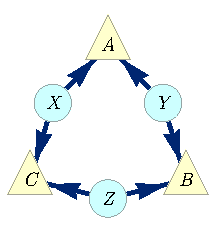
\includegraphics[scale=1]{TriDagRawALT.pdf}
\caption{The Triangle scenario.}\label{fig:TriMainDAG}
\end{minipage}
\hfill
\begin{minipage}[t]{0.43\linewidth}
\centering
\resizebox{\textwidth}{!}{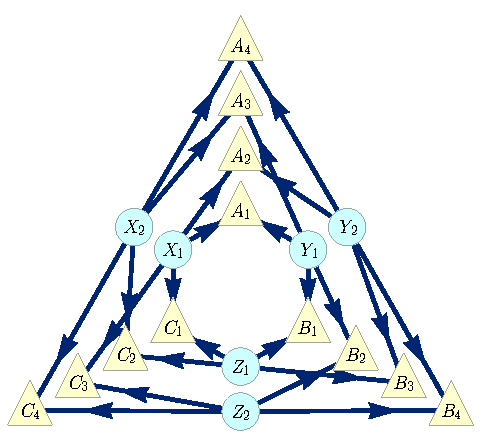
\includegraphics[scale=1]{TriDagFull222ALT.pdf}}
\caption{The Web inflation of the 
Triangle scenario where each latent node has been duplicated and each observed node has been quadrupled. The four copies of each observed node correspond to the four possible choices of parentage given the pair of copies of each latent parent of the observed node.}\label{fig:TriFullDouble}
\end{minipage}
\hfill
\begin{minipage}[t]{0.3\linewidth}
\centering
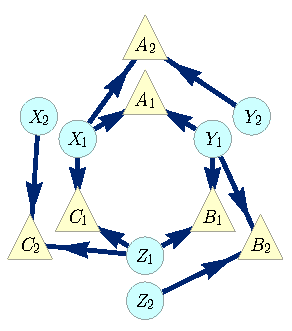
\includegraphics[scale=1]{TriDagSub222fixedcoordALT.pdf}
\caption{The Spiral inflation of the Triangle scenario.  Notably, this DAG is the ancestral subgraph of the set $\{ A_1 A_2 B_1 B_2 C_1 C_2\}$ in the Web inflation (\cref{fig:TriFullDouble}).}
 \label{fig:Tri222}
\end{minipage}
\end{figure}

\begin{figure}[hb]
\centering
\begin{minipage}[t]{0.3\linewidth}
\centering
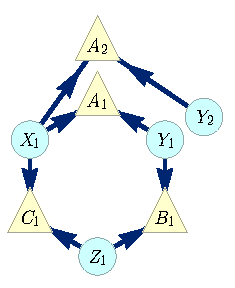
\includegraphics[scale=1]{broadcastingexamplenohighlightALT.pdf}
\caption{The Capped inflation of the Triangle scenario; notably also the ancestral subgraph of the set $\{ A_1 A_2 B_1 C_1\}$ in the Spiral inflation (\cref{fig:Tri222}).}
\label{fig:simpleinflation}
\end{minipage}\hfill
\begin{minipage}[t]{0.275\linewidth}
\centering
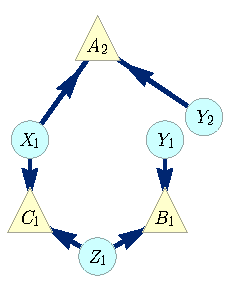
\includegraphics[scale=1]{nobroadcastingexamplenohighlightALT.pdf}
\caption{The Cut inflation of the Triangle scenario; notably also the ancestral subgraph of the set $\{ A_2 B_1 C_1\}$ in the Capped inflation (\cref{fig:simpleinflation}). Unlike the other examples, this inflation does not contain the Triangle scenario as a subgraph. 
}
\label{fig:simplestinflation}
\end{minipage}
\hfill
\begin{minipage}[t]{0.325\linewidth}
\centering
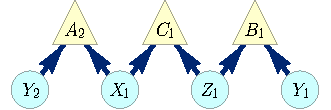
\includegraphics[scale=1]{TriDagSubA2B1C1.pdf}
\caption{A different depiction of the Cut inflation of \cref{fig:simplestinflation}. }\label{fig:TriDagSubA2B1C1}
\end{minipage}
\end{figure}

We now define the function $\mathsf{Inflation}_{G\to G'}$, that is, we specify how causal parameters are defined for a given inflation DAG in terms of causal parameters on the original DAG.

\begin{definition}
\label[definition]{def:inflat}
Consider causal models $M$ and $M'$ where $\DAG{M}=G$ and $\DAG{M'}=G'$, where $G'$ is an inflation of $G$. Then $M'$ is said to be the {\em \tblue{$G\to G'$ inflation of $M$}}, that is, $M' = \SmallNamedFunction[G\to G']{Inflation}{M}$,  if and only if for every node $A_i$ in $G'$, the manner in which $A_i$ depends causally on its parents within $G'$ is the same as the manner in which $A$ depends causally on its parents within $G$.  Noting that $A_i \sim A$ and that $\Pa[G']{A_i} \sim \Pa[G]{A}$ by~\cref{eq:definflationDAG}, one can formalize this condition as:
\begin{align}\label{eq:funcdependences}
 \forall A_i \in \nodes{G'}:\; \pfunc{A_i| \Pa[G']{A_i}}=\pfunc{A|\Pa[G]{A}}.
\end{align}
\end{definition}

For a given triple $G$, $G'$, and $M$, this definition specifies a unique inflation model $M'$, resulting in a well-defined function ${\operatorname{\mathsf{Inflation}}_{G\to G'}}$.

To sum up, the inflation of a causal model is a new causal model where (i) each variable in the original DAG may have counterparts in the inflation DAG with ancestral subgraphs mirroring those of the originals, and (ii) the manner in which a variable depends causally on its parents in the inflation DAG is given by the manner in which its counterpart in the original DAG depends causally on its parents. The operation of modifying a DAG and equipping the modified version with conditional probability distributions that mirror those of the original also appears in the \emph{do calculus} and \emph{twin networks} of~\citet{pearl2009causality}, and moreover bears some resemblance to the \emph{adhesivity} technique used in deriving non-Shannon-type entropic inequalities (\cref{sec:NonShannon}).

We are now in a position to describe the key property of the inflation of a causal model, the one that makes it useful for causal inference. With notation as in \cref{def:inflat}, let
$P_{\bm{U}}$ and $P_{\bm{U}'}$ denote marginal distributions on some $\bm{U}\subseteq\nodes{G}$ and $\bm{U}'\subseteq\nodes{G'}$, respectively. Then
\begin{align}\label{eq:coincidingdistrodef}
\quad\text{if }\quad \bm{U}'\sim \bm{U} \;\;\text{and}\;\; \ansubgraph[G']{\bm{U}'}\sim\ansubgraph[G]{\bm{U}}, \quad\text{then}\quad P_{\bm{U}'}=P_{\bm{U}}.
\end{align}
This follows from the fact that the distributions on $\bm{U}'$ and $\bm{U}$ depend only on their ancestral subgraphs and the parameters defined thereon, which by the definition of inflation are the same for $\bm{U}'$ and for $\bm{U}$.
It is useful to have a name for those sets of observed nodes in $G'$ which satisfy the antecedent of~\cref{eq:coincidingdistrodef}, that is, for which one can find a copy-index-equivalent set in the original DAG $G$ with a copy-index-equivalent ancestral subgraph.  We call such subsets of the observed nodes of $G'$ \tblue{injectable sets},
\begin{align}\begin{split}\label{eq:definjectable}
&\bm{U}'\in\SmallNamedFunction{InjectableSets}{G'} \\
&\quad\text{ iff }\quad \exists \bm{U}\subseteq \obsnodes{G} \;\; :\;\; \bm{U}'\sim\bm{U} \;\;\text{and}\;\; \ansubgraph[G']{\bm{U}'}\sim\ansubgraph[G]{\bm{U}}.
\end{split}\end{align}

Similarly,  those sets of observed nodes in the original DAG $G$ which satisfy the antecedent of~\cref{eq:coincidingdistrodef}, that is, for which one can find a corresponding set in the inflation DAG $G'$ with a copy-index-equivalent ancestral subgraph, we describe as \tblue{images of the injectable sets},
\begin{align}\begin{split}\label{eq:defimageinjectable}
& \bm{U}\in\SmallNamedFunction{ImagesInjectableSets}{G} \\
& \quad\text{ iff }\quad \exists \bm{U}' \subseteq \obsnodes{G'} \;\; :\;\; \bm{U'}\sim\bm{U} \;\;\text{and}\;\; \ansubgraph[G']{\bm{U}'}\sim\ansubgraph[G]{\bm{U}}.
\end{split}\end{align}
Clearly, $\bm{U}\in\SmallNamedFunction{ImagesInjectableSets}{G}$ iff $\exists \bm{U}' \subseteq \SmallNamedFunction{InjectableSets}{G'}$ such that $\bm{U}\sim \bm{U}'$.


For example in the Spiral inflation of the Triangle scenario depicted in~\cref{fig:Tri222}, the set $\brackets{A_1 B_1 C_1}$ is injectable because its ancestral subgraph is equivalent up to copy-indices to the ancestral subgraph of $\brackets{A B C}$ in the original DAG, and the set $\brackets{A_2 C_1}$ is injectable because its ancestral subgraph is equivalent to that of $\brackets{ A C}$ in the original DAG. 

A set of nodes in the inflation DAG can only be injectable if it contains at most one copy of any node from the original DAG. More strongly, it can only be injectable if its ancestral subgraph contains at most one copy of any observed or latent node from the original DAG.  
Thus, in \cref{fig:Tri222}, $\brackets{A_1 A_2 C_1}$ is not injectable because it contains two copies of $A$, and $\brackets{A_2 B_1 C_1}$ is not injectable because its ancestral subgraph contains two copies of $Y$. 

We can now express \cref{eq:coincidingdistrodef} in the language of injectable sets,
\begin{align}\label{keyinference}
P_{\bm{U}'}=P_{\bm{U}}\quad\text{if }  \;\; \bm{U}' \sim \bm{U}\;\; \text{and} \;\; \bm{U}'\in\SmallNamedFunction{InjectableSets}{G'}.
\end{align}

In the example of \cref{fig:Tri222}, injectability of the sets $\brackets{A_1 B_1 C_1}$ and $\brackets{A_2 C_1}$ thus implies that the marginals on each of these in anan model are equal to the marginals on their counterparts, $\brackets{A B C}$ and $\brackets{A C}$, in the original causal model, so that $P_{A_1 B_1 C_1} = P_{A B C}$ and $P_{A_2 C_1} = P_{A C}$.

\subsection{Witnessing incompatibility}
\label{subsec:witnessingincompat}

Finally, we can explain why inflation is relevant for deciding whether a distribution is compatible with a causal structure.  For a family of marginal distributions $\{ P_{\bm{U}} : \bm{U} \in \SmallNamedFunction{ImagesInjectableSets}{G}\}$ to be compatible with $G$, there must be a causal model $M$ that yields a joint distribution with this family as its marginals. Looking at the inflation model $M' = \SmallNamedFunction[G\to G']{Inflation}{M}$, \cref{keyinference} implies that $M'$ has the corresponding family of marginals given by $\{ P_{\bm{U}'} : \bm{U}' \in \SmallNamedFunction{InjectableSets}{G'}\}$ with $P_{\bm{U}'} = P_{\bm{U}}$ for $\bm{U}'\sim\bm{U}$, and thus this family is compatible with $G'$.

The same considerations apply for any collection of injectable sets:

\begin{lemma} \label[lemma]{mainlemma}
Let $G'$ be an inflation DAG of $G$. 
Let $S'  \subseteq \SmallNamedFunction{InjectableSets}{G'}$ be a collection of injectable sets, and let $S \subseteq \SmallNamedFunction{ImagesInjectableSets}{G}$ be the images of this collection.   If the family of marginal distributions $\{ P_{\bm{U}} : \bm{U} \in S \}$ is compatible with $G$, then the corresponding family of marginal distributions $\{ P_{\bm{U}'} : \bm{U}' \in S' \}$, defined via $P_{\bm{U}'}= P_{\bm{U}}$ for $\bm{U}' \sim \bm{U}$, is compatible with $G'$.
\end{lemma}

We have thereby related a question about compatibility with the original causal structure to one about compatibility with the inflated causal structure.  If one can show that the new compatibility question on $G'$ is answered in the negative, then one can infer that the original question is answered in the negative as well.    Some simple examples serve to illustrate the idea.





\begin{example}[\tred{Incompatibility of perfect three-way correlation with the Triangle scenario}]
\label{example:noGHZ}

\begin{figure}[bh]
\centering
\begin{minipage}[t]{0.45\linewidth}
\centering
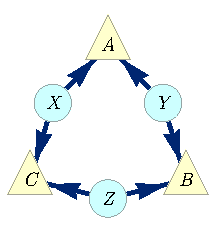
\includegraphics[scale=1]{TriDagRawALT.pdf}
\caption{The Triangle scenario. (Repeat of \cref{fig:TriMainDAG}.)}\label{fig:TriMainDAGv2}
\end{minipage}
\hfill
\begin{minipage}[t]{0.45\linewidth}
\centering
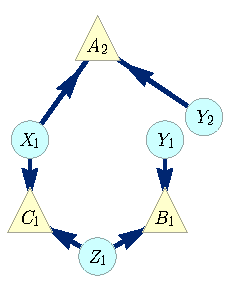
\includegraphics[scale=1]{nobroadcastingexamplenohighlightALT.pdf}
\caption{The Cut inflation of the Triangle scenario. (Repeat of \cref{fig:simplestinflation}.)}\label{fig:TriDagSubA2B1C1v2}
\end{minipage}
\end{figure}

Consider the following causal inference problem.  We are given a joint distribution of three binary variables, $P_{A B C}$, where the marginal on each variable is uniform and the three are perfectly correlated,
\begin{align}\label{eq:ghzdistribution1}
P_{A B C} =\frac{[000]+[111]}{2},\quad\text{i.e.,}\quad P_{A B C}(a b c)=\begin{cases}\tfrac{1}{2}&\text{if }\; a = b = c, \\ 0&\text{otherwise},\end{cases}
\end{align}
and one would like to determine whether it is compatible with the Triangle scenario (\cref{fig:TriMainDAGv2}). The notation $[abc]$ in \cref{eq:ghzdistribution1} is shorthand for the deterministic distribution where $A$, $B$, and $C$ take the values $a, b$, and $c$ respectively; in terms of the Kronecker delta, $[abc]:= \delta_{A,a} \delta_{B,b} \delta_{C,c}$.

Since there are no conditional independence relations among the observed variables in the Triangle scenario, there is no opportunity for ruling out the distribution on the grounds that it fails to satisfy the required conditional independences. 


To solve the causal inference problem, we consider the Cut inflation (\cref{fig:TriDagSubA2B1C1v2}). The injectable sets include $\brackets{A_2 C_1}$ and $\brackets{B_1 C_1}$.  Their images on the original DAG are $\brackets{AC}$ and $\brackets{BC}$, respectively.

We will show that the distribution of \cref{eq:ghzdistribution1} is not compatible with the Triangle scenario by demonstrating that the contrary assumption of compatibility implies a contradiction. If the distribution of Eq.~\eqref{eq:ghzdistribution1} is compatible, then so is the family of its marginals on $\brackets{AC}$ and $\brackets{BC}$, which are given by:
\begin{align*}
P_{A C} = P_{B C} = \frac{[00]+[11]}{2}.
\end{align*}
By \cref{mainlemma}, this compatibility assumption entails that the family of marginals
\begin{align}\label{ghzmarginals}
P_{A_2 C_1} = P_{B_1 C_1} = \frac{[00]+[11]}{2}
\end{align}
is compatible with the Cut inflation. We now show that this is actually not the case, thereby obtaining our contradiction.  It suffices to note that (i) the only joint distribution that exhibits perfect correlation between $A_2$ and $C_1$ and between $B_1$ and $C_1$ also exhibits perfect correlation between $A_2$ and $B_1$, and (ii) $A_2$ and $B_1$ have no common ancestor in the Cut inflation DAG and hence must be marginally independent in any distribution that is compatible with it. 

We have therefore certified that the distribution $P_{A B C}$ of~\cref{eq:ghzdistribution1} is not compatible with the Triangle scenario, recovering a result originally proven by \citet{steudel2010ancestors}.
\end{example}

\begin{example}[\tred{Incompatibility of the W-type distribution with the Triangle scenario}]
\label{example:noWdist}
\begin{figure}[bh]
\centering
\begin{minipage}[t]{0.45\linewidth}
\centering
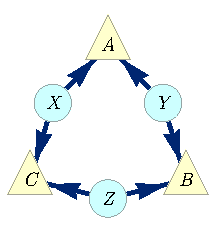
\includegraphics[scale=1]{TriDagRawALT.pdf}
\caption{The Triangle scenario. (Repeat of \cref{fig:TriMainDAG}.)}\label{fig:TriMainDAGv3}
\end{minipage}
\hfill
\begin{minipage}[t]{0.45\linewidth}
\centering
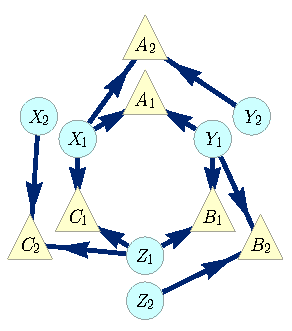
\includegraphics[scale=1]{TriDagSub222fixedcoordALT.pdf}
\caption{The Spiral inflation of the Triangle scenario. (Repeat of \cref{fig:Tri222}.)}\label{fig:Tri222v2}
\end{minipage}
\end{figure}


Consider another causal inference problem on the Triangle scenario, namely, that of determining whether the distribution 
\begin{align}\label{eq:wdistribution1}
P_{A B C}=\frac{[100]+[010]+[001]}{3},\quad\text{i.e.,}\quad P_{A B C}(a b c)=\begin{cases}\tfrac{1}{3}&\text{if }\; a + b + c = 1, \\ 0&\text{otherwise}.\end{cases}
\end{align}
is compatible with it. We call this the W-type distribution\footnote{The name stems from the fact that this distribution is reminiscent of 
the famous quantum state appearing in~\cite{3Qubits2Ways}, called the \emph{W state}.}. To settle this compatibility question, we consider the Spiral inflation of the Triangle scenario (\cref{fig:Tri222v2}).
The injectable sets in this case include $\{A_1 B_1 C_1\}$, $\{A_2 C_1\}$, $\{B_2 A_1\}$, $\{C_2 B_1\}$,  $\{A_2\}$, $\{B_2\}$ and $\{C_2\}$. 

Therefore, we turn our attention to determining whether the marginals of the W-type distribution on the images of these injectable sets are compatible with the Triangle scenario.  These marginals are:
\begin{align}
P_{A B C}&= \frac{[100]+[010]+[001]}{3}, \label{V4}\\
P_{A C}= P_{B A} = P_{C B} & = \frac{[10]+[01]+[00]}{3}, \label{V1}\\
P_{A}= P_B = P_C & = \frac{2}{3}[0] + \frac{1}{3}[1]. \label{V5}
\end{align}
By \cref{mainlemma}, this compatibility holds only if the associated marginals for the injectable sets, namely, 
\begin{align}
P_{A_1 B_1 C_1}&= \frac{[100]+[010]+[001]}{3}, \label{W4}\\
P_{A_2 C_1} = P_{B_2 A_1} = P_{C_2 B_1} & = \frac{[10]+[01]+[00]}{3}, \label{W1}\\
P_{A_2} = P_{B_2} = P_{C_2} & = \frac{2}{3}[0] + \frac{1}{3}[1], \label{W5}
\end{align}
are compatible with the Spiral inflation (\cref{fig:Tri222v2}). \cref{W1}
implies that $C_1 = 0$ whenever $A_2 = 1$. It similarly implies that $A_1 = 0$ whenever $B_2 = 1$, and that $B_1 = 0$ whenever $C_2 = 1$, 
\begin{align} 
\begin{split}\label{Ws}
&A_2  = 1 \:\implies\: C_1 = 0,\\
&B_2 = 1 \:\implies\: A_1 = 0,\\
&C_2  = 1 \:\implies\: B_1  = 0.
\end{split}
\end{align}
Our inflation DAG is such that $A_2$, $B_2$ and $C_2$ have no common ancestor and consequently are marginally independent in any distribution compatible with it. Together with \cref{W5}, this implies that
\begin{align} \label{WW2}
\text{Sometimes} \quad &A_2  = 1\,\text{ and }\, B_2  = 1\,\text{ and }\, C_2  = 1.
\end{align} 
Finally, \cref{Ws} together with \cref{WW2} entails
\begin{align} \label{WW3}
\text{Sometimes} \quad &A_1  = 0\,\text{ and }\, B_1  = 0\,\text{ and }\, C_1  = 0.
\end{align}
This, however, contradicts~\cref{W4}.  Consequently, the family of marginals described in \cref{W4,W1,W5} is \emph{not} compatible with the DAG of~\cref{fig:Tri222v2}.  By \cref{mainlemma}, this implies that the family of marginals described in \cref{V4,V1,V5}---and therefore the W-type distribution of which they are marginals---is not compatible with the Triangle scenario.

To our knowledge, this is a new result. In fact, the incompatibility of the W-type distribution with the Triangle scenario cannot be derived via any of the following existing causal inference techniques:
\begin{enumerate}
\item Checking conditional independence relations is not relevant here, as there are \emph{no} conditional independence relations implied between any observed variables in the Triangle scenario. 
\item The relevant Shannon-type entropic inequalities for the Triangle scenario have been classified, and they do not witness the incompatibility either~\cite{fritz2013marginal,chaves2014novel,chaves2014informationinference}. 
\item Moreover, \emph{no} entropic inequality can witness the W-type distribution as unrealizable. \citet{weilenmann2016entropic} have constructed an inner approximation to the entropic cone of the Triangle causal structure, and the W-distribution lies inside this. In other words, a distribution with the same entropic profile as the W-type distribution \emph{can} arise from the Triangle scenario.
\item The newly-developed method of covariance matrix causal inference due to \citet{kela2016covariance}, which gives tighter constraints than entropic inequalities for the Triangle scenario, also cannot detect the incompatibility.
\end{enumerate}
Therefore, in this case at least, the inflation technique appears to be more powerful. 

We have arrived at our incompatibility verdict by combining inflation with reasoning reminiscent of  Hardy's version of Bell's theorem~\cite{L.Hardy:PRL:1665,Mansfield2012}. \cref{sec:TSEM} will present a generalization of this kind of argument and its applications to causal inference. 
\end{example}

\begin{example}[\tred{Incompatibility of PR-box correlations with the Bell scenario}]
\label{example:noPR}

Bell's theorem~\cite{bell1964einstein,Brunner2013Bell,bell1966lhvm,CHSHOriginal} concerns the question of whether the distribution obtained in an experiment involving a pair of systems that are measured at space-like separation is compatible with a causal structure of the form of \cref{fig:NewBellDAG1}. Here, the observed variables are $\brackets{A,B,X,Y}$, and $\Lambda$ is a latent variable acting as a common cause of $A$ and $B$. We shall term this causal structure the \emph{Bell scenario}. While the causal inference formulation of Bell's theorem is not the traditional one, several recent articles have introduced and advocated this perspective~[\citealp{WoodSpekkens}~(Fig.~19), \citealp{pusey2014gdag}~(Fig.~E\#2), \citealp{BeyondBellII}~(Fig.~1), \citealp{chaves2014novel}~(Fig.~1), \citealp{wolfe2015nonconvexity}~(Fig.~2b), \citealp{steeg2011relaxation}~(Fig.~2)].  


\begin{figure}[ht]
\centering
\begin{minipage}[t]{0.45\linewidth}
\centering
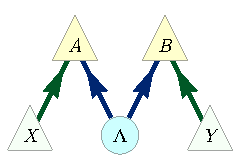
\includegraphics[scale=1]{BellDagRaw.pdf}
\caption{The causal structure of the bipartite Bell scenario. The local outcomes $A$ and $B$ of Alice's and Bob's measurements is assumed to be a function of some latent common cause and their independent local experimental settings $X$ and $Y$.}\label{fig:NewBellDAG1}
\end{minipage}
\hfill
\begin{minipage}[t]{0.45\linewidth}
\centering
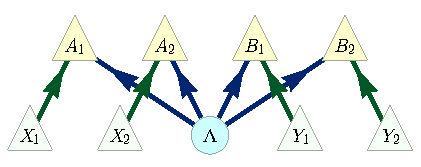
\includegraphics[scale=1]{BellDagCopy.pdf}
\caption{An inflation DAG of the bipartite Bell scenario, where both local settings and outcome variables have been duplicated.}\label{fig:BellDagCopy1}
\end{minipage}
\end{figure}


We consider the distribution ${P_{A B X Y} = P_{A B | X Y} P_{X} P_{Y}}$, where $P_{X}$ and $P_{Y}$ are arbitrary full-support distributions\footnote{In the literature on the Bell scenario, these variables are known as ``settings''. Generally, we may think of observed root variables as settings, coloring them light green in the DAG figures. They are natural candidates for variables to condition on.} over the binary variables $X$ and $Y$, and
\begin{align}\begin{split}\label{eq:PRbox}
 p_{\text{PR}}\parens{a b |x y}=\frac{[00|00]+[11|00]+[00|10]+[11|10]+[00|01]+[11|01]+[01|11]+[10|11]}{8}\\
P_{A B | X Y}\parens{a b |x y}=\begin{cases}\tfrac{1}{2}&\text{if }\; a \oplus b = x \cdot y , \\ 0&\text{otherwise},\end{cases}
\end{split}\end{align}
a conditional distribution that was discovered by Tsirelson~\cite{Tsirelson1980} and later independently by Popescu and Rohrlich~\cite{PROriginal,PRUnit}. It has become known in the field of quantum foundations as the \emph{PR-box} after the latter authors.\footnote{The PR-box is of interest because it represents a manner in which experimental observations could deviate from the predictions of quantum theory while still being consistent with relativity.}

The Bell scenario implies nontrivial conditional independences\footnote{Recall that variables $X$ and $Y$ are conditionally independent given $Z$ if $P_{XY|Z}(xy|z) = P_{X|Z}(x|z) P_{Y|Z}(y|z)$ for all $z$ with $P_{Z}(z)>0$. Such a conditional independence is denoted by $X\indep Y \:|\: Z$.} among the observed variables, namely, $X \indep Y$, $A \indep Y| X$, and\footnote{In the context of a Bell experiment, where $\{X,A\}$ are space-like separated from $\{Y,B\}$, the conditional independences $A \indep Y| X$ and $B \indep X|Y$ encode the impossibility of sending signals faster than the speed of light.} $B \indep X|Y$, as well as those that can be generated from these by the semi-graphoid axioms \cite{WoodSpekkens}.
It is straightforward to check that these conditional independence relations are respected by the $P_{ABXY}$ resulting from~\cref{eq:PRbox}. It is well-known that this distribution is nonetheless incompatible with the Bell scenario, for example since it violates the CHSH inequality.
Here we prove this incompatibility via the inflation technique, using the inflation of the Bell scenario depicted in \cref{fig:BellDagCopy1}.

We begin by noting that $\{A_1 B_1 X_1 Y_1\}$, $\{A_2 B_1 X_2 Y_1\}$, $\{A_1 B_2 X_1 Y_2\}$, $\{A_2 B_2 X_2 Y_2\}$, $\{X_1\}$, $\{X_2\}$, $\{Y_1\}$, and $\{Y_2\}$ are all injectable sets. 
By \cref{mainlemma}, it follows that any causal model that recovers $P_{ABXY}$ inflates to a model that results in marginals
\begin{align}
P_{A_1 B_1 X_1 Y_1}=P_{A_2 B_1 X_2 Y_1}=P_{A_1 B_2 X_1 Y_2}=P_{A_2 B_2 X_2 Y_2}&=P_{A B X Y},\label{PR1}\\
P_{X_1}=P_{X_2}=P_X, \qquad P_{Y_1}=P_{Y_2}&=P_Y.\label{PR5}
\end{align}
Using the definition of conditional probability, we infer that
\begin{align}
P_{A_1 B_1 |X_1 Y_1}=P_{A_2 B_1 |X_2 Y_1}=P_{A_1 B_2 |X_1 Y_2}=P_{A_2 B_2 |X_2 Y_2}=P_{A B |X Y}\label{PRb}.
\end{align}
Because $\{X_1\}$, $\{X_2\}$, $\{Y_1\}$, and $\{Y_2\}$ have no common ancestor in the inflation DAG, these variables must be marginally independent in any distribution compatible with the inflation DAG. This applies in particular to the inflation model, so that $P_{X_1 X_2 Y_1 Y_2} = P_{X_1} P_{X_2} P_{Y_1} P_{Y_2}$. Given the assumption that the distributions $P_{X}$ and $P_{Y}$ have full support, it follows from~\cref{PR5} that
\begin{align}\label{PRs}
\text{Sometimes} \quad &X_1 = 0\,\text{ and }\, X_2  =1\,\text{ and }\, Y_1  = 0\,\text{ and }\, Y_2  = 1.
\end{align} 
On the other hand, from~\cref{PRb} together with  the definition of PR-box,~\cref{eq:PRbox}, we conclude that 
\begin{align} 
\begin{split}
\label{PRsi}
&X_1  = 0,\: Y_1  = 0 \:\implies\: A_1 = B_1,\\
&X_1  = 0,\: Y_2  = 1 \:\implies\: A_1 = B_2,\\
&X_2  = 1,\: Y_1  = 0 \:\implies\: A_2 = B_1,\\
&X_2  = 1,\: Y_2  = 1 \:\implies\: A_2\ne B_2.
\end{split}
\end{align}
Combining this with~\cref{PRs}, we obtain
\begin{align}
\text{Sometimes} \quad &A_1 = B_1\,\text{ and }\, A_1 = B_2\,\text{ and }\, A_2 = B_1\,\text{ and }\, A_2\neq B_2.
\end{align} 
No values of $A_1$, $A_2$, $B_1$, and $B_2$ can jointly satisfy these conditions. So we have reached a contradiction, showing that our original assumption of compatibility of $P_{ABXY}$ with the Bell scenario must have been false.

The structure of this proof parallels that of standard proofs of the incompatibility of the PR-box with the Bell scenario. Standard proofs focus on a set of variables $\{A_0 A_1 B_0 B_1\}$ where $A_x$  is the value of $A$ when $X=x$ and $B_y$  is the value of $B$ when $Y=y$, and note that  the distribution
 $\sum_{\lambda} P(A_0|\lambda)P(A_1|\lambda)P(B_0|\lambda)P(B_1|\lambda)P(\lambda)$

 is a joint distribution of these four variables for which the marginals on pairs  $\{ A_0 B_0\}$, $\{ A_0 B_1\}$, $\{ A_1 B_0\}$ and $\{ A_1 B_1\}$ are those corresponding to the conditional distribution describing the PR-box, \cref{eq:PRbox}. Finally, the existence of such a joint distribution rules out the possibility of having $A_1 = B_1$, $A_1 = B_2$, $A_2 = B_1$ but $ A_2\neq B_2$, and therefore shows that the PR-box distribution is incompatible with the Bell scenario~\cite{LSW,roberts_thesis}. In light of our use of \cref{PRs}, our reasoning is really the same argument in disguise.

\cref{sec:Bellscenarios} shows that the inflation of~\cref{fig:BellDagCopy1}, with the number of copies corresponding to the cardinality of $X$ and $Y$, is enough to witness the incompatibility of any distribution that is incompatible with the Bell scenario.
\end{example}

\subsection{Deriving causal compatibility inequalities}
\label{Sec:DerivingInequalities}

The inflation technique can be used not only to witness the incompatibility of a given distribution with a given causal structure, but also to derive generally applicable necessary conditions that a distribution must satisfy to be compatible with the given causal structure. When these conditions are expressed as inequalities, we will refer to them as {\em causal compatibility inequalities}.  Formally, we have:

\begin{definition}
Let $G$ be a causal structure and $S \subseteq 2^{\obsnodes{G}}$.  Let $I_S$ denote an inequality that operates on a family of marginal distributions  $\{ P_{\bm{U}}: \bm{U} \in S\}$.  Then $I_S$ is a \tblue{\em causal compatibility inequality for the causal structure $G$} whenever it is satisfied by every family of marginal distributions $\{ P_{\bm{U}}: \bm{U} \in S\}$ that is compatible with $G$.
\end{definition}
While violation of a causal compatibility inequality witnesses the incompatibility with the causal structure, satisfaction of the inequality does not guarantee compatibility.  This is the sense in which it merely provides a {\em necessary} condition for compatibility. 

The inflation technique is useful for deriving causal compatibility inequalities because of the following consequence of  \cref{mainlemma}:

\begin{corollary} \label[corollary]{maincorollary}
Suppose that $G'$ is an inflation of $G$. Let $S'  \subseteq \SmallNamedFunction{InjectableSets}{G'}$ be a family of injectable sets and $S \subseteq \SmallNamedFunction{ImagesInjectableSets}{G}$ the images of members of $S'$.
Let $I_{S'}$ be a causal compatibility inequality for $G'$ operating on families $\{ P_{\bm{U}'} : \bm{U}' \in S'\}$. Define an inequality $I_S$ as follows: in the functional form of $I_{S'}$, replace every occurrence of a term $P_{\bm{U}'}$ by $P_{\bm{U}}$ for the unique $\bm{U}\in S$ with $\bm{U} \sim \bm{U}'$. Then $I_S$ is a causal compatibility inequality for $G$ operating on families $\{ P_{\bm{U}} : \bm{U}\in S\}$.
\end{corollary}

The proof is as follows.  Suppose that the family $\{ P_{\bm{U}} : \bm{U} \in S\}$ is compatible with $G$.  By \cref{mainlemma}, it follows that the family $ \{ P_{\bm{U}'} : \bm{U}' \in S'\}$ where $P_{\bm{U}'}:= P_{\bm{U}}$ for $\bm{U}' \sim \bm{U}$  is compatible with $G'$.  Since $I_{S'}$ is a causal compatibility inequality for $G'$, it follows that $\{ P_{\bm{U}'} : \bm{U}' \in S'\}$ satisfies $I_{S'}$.  But by the definition of $I_{S}$, its evaluation on $\{ P_{\bm{U}} : \bm{U} \in S\}$ is equal to $I_{S'}$ evaluated on $\{ P_{\bm{U}'} : \bm{U}' \in S'\}$. It therefore follows that $\{ P_{\bm{U}} : \bm{U} \in S\}$ satisfies $I_{S}$. Since $\{ P_{\bm{U}} : \bm{U}\in S\}$ was an arbitrary family compatible with $G$, we conclude that $I_{S}$ is a causal compatibility inequality for $G$.  

We now present some simple examples of causal compatibility inequalities for the Triangle scenario that one can derive from the inflation technique via \cref{maincorollary}. Some terminology and notation will facilitate their description. We refer to a pair of nodes which do not share any common ancestor as being \tblue{ancestrally independent}. This is equivalent to being $d$-separated by the empty set~\cite{pearl2009causality,spirtes2011causation,studeny2005probabilistic,koller2009probabilistic}.  Given that the conventional notation for $X$ and $Y$ being $d$-separated by $Z$ in the DAG $G$ is $X\perp_G Y|Z$, we denote $X$ and $Y$ being ancestrally independent within $G$ as $X\perp_G Y$.  Generalizing to sets, $\bm{U}\aindep_G \bm{V}$ indicates that no node in $\bm{U}$ shares a common ancestor with any node in $\bm{V}$ within the DAG $G$, 
\begin{align}
\bm{U}\aindep_G \bm{V} \quad \text{iff} \quad \An[G]{\bm{U}}\cap\An[G]{\bm{V}}=\emptyset.
\end{align}
Furthermore, the notation ${\bm{U}\aindep_G \bm{V}\aindep_G \bm{W}}$ should be understood as indicating that $\bm{U}\aindep_G \bm{V}$ and $\bm{V}\aindep_G \bm{W}$ and $\bm{U}\aindep_G \bm{W}$.

\begin{example}[\tred{A causal compatibility inequality in terms of \tpurp{\emph{correlators}}}]
\label{example:polytriangle}

As in \cref{example:noGHZ} of the previous section, consider the Cut inflation of the Triangle scenario (\cref{fig:TriDagSubA2B1C1v2}), where all observed variables are binary. For technical convenience, we assume that they take values in the set $\{-1,+1\}$, rather than taking values in $\{0,1\}$ as was presumed in the last section. 

The injectable sets that we make use of are $\brackets{A_2 C_1}$, $\brackets{B_1 C_1}$, $\{ A_2\}$, and  $\brackets{B_1}$. From \cref{maincorollary}, any causal compatibility inequality for the inflation DAG that operates on the marginal distributions of $\brackets{A_2 C_1}$, $\brackets{B_1 C_1}$, $\{ A_2\}$, and  $\brackets{B_1}$ will yield a causal compatibility inequality for the original DAG that can be evaluated on the marginal distributions on $\brackets{A C}$, $\brackets{B C}$, $\brackets{A}$, and  $\brackets{B}$. We begin by noting that for {\em any} distribution on three binary variables $\{A_2 B_1 C_1\}$, that is, {\em regardless} of the causal structure in which they are embedded, the marginals on $\brackets{A_2 C_1}$, $\brackets{B_1 C_1}$ and $\brackets{A_2 B_1}$ satisfy the following inequality for expectation values~\cite{pitowsky_boole_1994,Pitowsky1989,kellerer_marginal_1964,leggett_garg_1985,araujo_cycle_2013},
\begin{equation}
	\label{eq:polymonogamyraw}
	\langle A_2 C_1\rangle + \langle B_2 C_1 \rangle - \langle A_2 B_1 \rangle \leq 1.
\end{equation}
This is an example of a constraint on pairwise correlators that arises from the presumption that they are consistent with a joint distribution. (The problem of deriving such constraints is the {\em marginal constraint problem}, discussed in detail in \cref{sec:ineqs}.)

But in the Cut inflation of the Triangle scenario~(\cref{fig:TriDagSubA2B1C1v2}) $A_2$ and $B_1$ have no common ancestor and consequently any distribution compatible with this DAG must make $A_2$ and $B_1$ marginally independent.  In terms of correlators, this can be expressed as 
\begin{align}\label{corrfact}
A_2 \aindep B_1 \implies  \langle A_2 B_1 \rangle =  \langle A_2\rangle \langle B_1 \rangle.
\end{align}
Substituting this into~\cref{eq:polymonogamyraw}, we have
\begin{equation}
	\langle A_2 C_1\rangle + \langle B_2 C_1 \rangle   \leq 1 + \langle A_2 \rangle \langle B_1\rangle.
\end{equation}
This is an example of a simple but nontrivial causal compatibility inequality for the DAG of~\cref{fig:TriDagSubA2B1C1v2}. Finally, by \cref{maincorollary},  we infer that 
\begin{equation}
	\label{eq:polymonogamy}
	\langle A C\rangle + \langle B C\rangle \leq 1 + \langle A\rangle \langle B\rangle
\end{equation}
is a causal compatibility inequality for the Triangle scenario.   This inequality expresses the fact that as long as $A$ and $B$ are not completely biased, there is a tradeoff between the strength of $AC$ correlations and the strength of $BC$ correlations.   

Given the symmetry of the Triangle scenario under permutations and sign flips of $A$, $B$ and $C$, it is clear that the image of inequality~\cref{eq:polymonogamy} under any such symmetry is also a valid causal compatibility inequality.  Together, these inequalities constitute a type of monogamy\footnote{We are here using the term ``monogamy'' in the same sort of manner in which it is used in the context of entanglement theory~\cite{horo4}.}  of correlations in the Triangle scenario with binary variables:  if any two observed variables with unbiased marginals are perfectly correlated, then they are both uncorrelated with the third.
\end{example}

\begin{example}[\tred{A causal compatibility inequality in terms of \tpurp{\emph{entropic quantities}}}]
\label{ex:entropic}

One way to derive constraints that are independent of the cardinality of the observed variables is to express these in terms of the mutual information between observed variables rather than in terms of correlators.  The inflation technique can also be applied to achieve this.
To see how this works in the case of the Triangle scenario, consider again the Cut inflation~(\cref{fig:TriDagSubA2B1C1v2}).  

One can follow the same logic as in the preceding example, but starting from a different constraint on marginals.  For any distribution on three variables $\{A_2 B_1 C_1\}$ of arbitrary cardinality (again, regardless of the causal structure in which they are embedded), the marginals on $\brackets{A_2 C_1}$, $\brackets{B_1 C_1}$ and $\brackets{A_2 B_1}$ satisfy the inequality~\cite[Eq.~(29)]{fritz2013marginal}
\label{example:entropic}\begin{align}\label{eq:MIraw}
	I(A_2 : C_1) + I(C_1 : B_1) - I(A_2 : B_1) \leq H(C_1),	
\end{align}
where $H(X)$ denotes the Shannon entropy of the distribution of $X$, and $I(X: Y)$ denotes the mutual information between $X$ and $Y$ with respect to the marginal on $X$ and $Y$. The fact that $A_2$ and $B_1$ have no common ancestor in the inflation DAG implies that in any distribution that is compatible with the inflation DAG, $A_2$ and $B_1$ are marginally independent.  This is expressed entropically as the vanishing of their mutual information, 
\begin{align}\label{entropicfact}
A_2 \aindep B_1 \implies  I(A_2 : B_1)  =0.
\end{align}
Substituting the latter equality into~\cref{eq:MIraw}, we have
\begin{align}
	I(A_2 : C_1) + I(C_1 : B_1)  \leq H(C_1).
\end{align}
This is another example of a nontrivial causal compatibility inequality for the DAG of~\cref{fig:TriDagSubA2B1C1v2}. By \cref{maincorollary}, it follows that 
\begin{align}\label{eq:monogomyofcorrelations}
	I(A : C) + I(C : B) \leq H(C)
\end{align}
is also a causal compatibility inequality for the Triangle scenario.  This inequality was originally derived in~\cite{fritz2012bell}. Our rederivation in terms of inflation coincides with the proof found by~\citet{pusey2014gdag}.
\end{example}

\begin{example}[\tred{A causal compatibility inequality in terms of \tpurp{\emph{joint probabilities}}}]
\label{example:probineq}
Consider the Spiral inflation of the Triangle scenario (\cref{fig:Tri222v2}) with the injectable sets $\{A_1 B_1 C_1\}$, $\{A_1 B_2\}$, $\{B_1 C_2\}$, $\{ A_1, C_2\}$, $\{A_2\}$, $\{B_2\}$, and $\{C_2\}$. We derive a causal compatibility inequality under the assumption that the observed variables are binary, adopting the convention that they take values in $\{0,1\}$.

We begin by noting that the following is a constraint that holds for any joint distribution of $\{A_1 B_1 C_1 A_2 B_2 C_2\}$, regardless of the causal structure, 
\begin{align}\label{eq:FritzF3raw}
	P_{A_2 B_2 C_2}(111) \leq P_{A_1 B_2 C_2}(111) + P_{B_1 C_2 A_2}(111) + P_{A_2 C_1 B_2}(111) + P_{A_1 B_1 C_1}(000).
\end{align}
To prove this claim, it suffices to check that the inequality holds for each of the $2^6$ deterministic assignments of outcomes to $\{A_1 B_1 C_1 A_2 B_2 C_2\}$, from which the general case follows by linearity.  A more intuitive proof will be provided in~\cref{sec:TSEM}.

Next, we note that certain sets of variables have no common ancestors with other sets of variables in the inflation DAG, which implies marginal independences resulting in factorization of distributions,
\begin{align}\begin{split}\label{eq:tri222fac}
A_1 B_2 \aindep C_2 \:\implies\:	P_{A_1 B_2 C_2} &= P_{A_1 B_2} P_{C_2}, \\
B_1 C_2 \aindep A_2 \:\implies\:	P_{B_1 C_2 A_2} &= P_{B_1 C_2} P_{A_2}, \\
A_2 C_1 \aindep B_2 \:\implies\:	P_{A_2 C_1 B_2} &= P_{A_2 C_1} P_{B_2}, \\
A_2 \aindep B_2 \aindep C_2 \:\implies\:	P_{A_2 B_2 C_2} &= P_{A_2} P_{B_2} P_{C_2} .
\end{split}\end{align}
Substituting these equations into~\cref{eq:FritzF3raw}, we obtain the polynomial inequality
\begin{equation}
	P_{A_2}(1) P_{B_2}(1) P_{C_2}(1) \leq P_{A_1 B_2}(11) P_{C_2}(1) + P_{B_1 C_2}(11) P_{A_2}(1) + P_{A_2 C_1}(11) P_{B_2}(1) + P_{A_1 B_1 C_1}(000).
\end{equation}
This, therefore, is a causal compatibility inequality for the DAG of \cref{fig:Tri222v2}. Finally, by \cref{maincorollary}, we infer that 
\begin{equation}\label{eq:FritzF3}
	P_{A}(1) P_{B}(1) P_{1}(0) \leq P_{AB}(11) P_C(1) + P_{BC}(11) P_A(`) + P_{AC}(11) P_B(1) + P_{ABC}(000)
\end{equation}
is a causal compatibility inequality for the Triangle scenario.  

What is distinctive about this inequality is that---through the presence of the term $P_{ABC}(000)$---it takes into account genuine three-way correlations, while our earlier inequalities only depend on the two-variable marginals.  This inequality is strong enough to demonstrate the incompatibility of the W-type distribution of \cref{eq:wdistribution1} with the Triangle scenario: for this distribution, the right-hand side of the inequality vanishes while the left-hand side does not.
\end{example}

Of the known techniques for witnessing the incompatibility of a distribution with a DAG or deriving necessary conditions for compatibility, the most straightforward is to consider the constraints implied by ancestral independences among the observed variables of the DAG. 
The constraints derived in the last two sections have all made use of this basic technique, but at the level of the inflation DAG rather than the original DAG.  The constraints that one thereby infers for the original DAG reflect facts about its causal structure that cannot be expressed in terms of ancestral independences among its observed variables.  The inflation technique exposes these facts in the ancestral independences among observed variables of the inflation DAG.

In the rest of this article, we shall continue to rely only on the ancestral independences among observed variables within the inflation DAG to infer compatibility constraints on the original DAG.   Nonetheless, it seems plausible that the inflation technique can also amplify the power of {\em other} techniques that do not merely consider ancestral independences among the observed variables.  We consider some prospects in \cref{sec:otherprospects}.

\section{Systematically witnessing incompatibility and deriving inequalities}
\label{sec:ineqs}

This section considers the problem of how to generalize the above examples of causal inference via the inflation technique to a systematic procedure. We start by introducing the crucial concept of \emph{pre-injectable set}, which figures implicitly in our earlier example. By reformulating \cref{example:noGHZ}, we sketch our general method and explain why solving a \emph{marginal problem} is an essential subroutine of our method. Subsequently, \cref{step:findpreinjectable} explains how to find all of the pre-injectable sets for a given inflation DAG systematically. \cref{step:marginalsproblem} describes how to solve any sort of marginal problem. This may involve determining all the facets of the \emph{marginal polytope}, which is computationally costly (\cref{sec:projalgorithms}).  It is therefore useful to also consider relaxations of the marginal problem that are more tractable by deriving valid linear inequalities which may or may not bound the marginal polytope tightly. We describe one such approach based on possibilistic Hardy-type paradoxes and the hypergraph transversal problem in \cref{sec:TSEM}.

As far as causal compatibility inequalities are concerned, we limit ourselves to those expressed in terms of probabilities\footnote{Or, for binary variables, equivalently in terms of correlators, as in the first example of \cref{Sec:DerivingInequalities}.}, as these are generally the most powerful. However, essentially the same techniques can be used to derive inequalities expressed in terms of entropies~\cite{fritz2013marginal}, as demonstrated in \cref{ex:entropic}. 

In the examples from the previous section, the initial inequality---a constraint upon marginals that is independent of the causal structure---involves sets of observed variables that are \emph{not} all injectable sets.  Each of these sets can, however, be partitioned into disjoint subsets each of which {\em is} injectable such that the partitioning represents ancestral independence in the inflation DAG. Also in \cref{example:noGHZ}, the set $\{ A_2 B_1\}$ is not injectable, but it can be partitioned into the singleton sets $\{ A_2 \}$ and $\{ B_1\}$ which are ancestrally independent and each of which is injectable.  It is useful to have a name for such sets of observed variables: we call them \tblue{pre-injectable}. So for any $\bm{U}'$ in the inflation DAG $G'$,
\begin{align}\label{eq:defpreinj}
\begin{split}
\bm{U}'\in & \SmallNamedFunction{PreInjectableSets}{G'} \\
	& \quad\text{ iff }\quad  \exists \{ \bm{U}'_i \in \SmallNamedFunction{InjectableSets}{G'} \} \quad \text{s.t.}\quad \bm{U}'=\bigcup_i \bm{U}'_i  \quad\text{and} \quad  \forall i\ne j: \bm{U}'_i \aindep_{G'} \bm{U}'_j.
\end{split}
\end{align}
For example, every injectable set is trivially pre-injectable.  A pre-injectable set is \emph{maximal} if it is not a proper subset of another pre-injectable set.

Because ancestral independence in the DAG implies statistical independence for any distribution compatible with the DAG, it follows that  if 
$\bm{U}'$ is a pre-injectable set with ancestrally independent components $\bm{U}'_1,\ldots,\bm{U}'_n$, then we have the factorization
\begin{align}\label{eq:preinjfactor}
P_{\bm{U}'} = P_{\bm{U}'_1} \cdots P_{\bm{U}'_n}
\end{align}
for any distribution compatible with $G'$. The situation, therefore, is this: for any constraint that one can derive for the marginals on the pre-injectable sets based on the existence of a joint distribution---and hence without reference to the causal structure---one can infer a constraint that {\em does} refer to the causal structure by substituting within the derived constraint a factorization of the form of~\cref{eq:preinjfactor}. As a build-up to our exposition of a systematic application of the inflation technique, we now revisit \cref{example:noGHZ}.

As before, we infer the marginal distributions on injectable sets,
\begin{equation}
P_{A_2 C_1} = P_{B_1 C_1} = \frac{1}{2} [00] +\frac{1}{2} [11], \qquad P_{A_2} = P_{B_1}=\frac{1}{2} [0] +\frac{1}{2} [1],
\label{marginals1}
\end{equation}
from the given W distribution of \cref{eq:ghzdistribution1} via \cref{mainlemma}. From the fact that $A_2$ and $B_1$ are ancestrally independent, we also infer the distribution on the pre-injectable set $\{A_2 B_1\}$ as
\begin{equation}
P_{A_2 B_1} = P_{A_2}P_{B_1} = \left(\frac{1}{2} [0] +\frac{1}{2} [1]\right)\times\left(\frac{1}{2} [0] +\frac{1}{2} [1]\right)=\frac{1}{4} [00]+\frac{1}{4} [01]+\frac{1}{4} [10]+\frac{1}{4} [11].
\label{marginals2}
\end{equation}
The incompatibility with the Triangle scenario then follows from the fact there is no three-variable distribution $P_{A_2 B_1 C_1}$ that would have the two-variable marginals of \cref{marginals1,marginals2}. For as we noted in our prior discussion of this example, the perfect correlation between $A_2$ and $C_1$ exhibited by $P_{A_2 C_1}$ and the perfect correlation between $B_1$ and $C_1$ exhibited by $P_{B_1 C_1}$ would entail perfect correlation between $A_2$ and $B_1$ as well, but this is at odds with \eqref{marginals2}. It follows that there is no joint distribution that has the distributions of \cref{marginals1,marginals2} as its marginals. 

Generalizing to an arbitrary DAG, therefore, the procedure is as follows:
\begin{enumerate}
\item Based on the inflation DAG, identify the pre-injectable sets and how they each partition into injectable sets.
\item From the given distribution on the DAG, infer the family of marginal distributions on the pre-injectable sets of the inflation DAG as follows: the distribution on any injectable set is equal to the corresponding distribution on its image in the original DAG; the distribution on any pre-injectable set is the product of the distributions on the injectable sets into which it is partitioned.
\item Determine whether the family of distributions obtained in step 2 are the marginals of a single joint distribution. If no, then the original distribution is incompatible with the original DAG; otherwise, it may or may not be compatible.
\end{enumerate}
The procedure for systematically deriving causal compatibility inequalities is analogous: instead of determining whether a given family of distributions can arise as marginals of a joint distribution, one rater determines all \emph{constraints} that such a family must satisfy in order to arise from a joint distribution. These constraint translate into causal compatibility inequalities for the inflation DAG via the ancestral independences of \cref{eq:preinjfactor}, and then into causal compatibility inequalities for the original DAG via \cref{maincorollary}.

The pre-injectable sets play a crucial role in linking the original DAG with the inflation DAG: they are precisely those sets of variables whose joint distributions in the inflation model are fully specified by the causal model on the original DAG, as they can be computed using \cref{eq:preinjfactor} and \cref{mainlemma}. So we begin with the problem of identifying the pre-injectable sets systematically.

\subsection{Identifying the pre-injectable sets}
\label{step:findpreinjectable}

To identify the pre-injectable sets of an inflation DAG $G'$, we must first identify the injectable sets. This problem can be reduced to identifying the injectable pairs of nodes, because if all of the pairs in a set of nodes are injectable, then so too is the set itself. This can be proven as follows.   
Let $\varphi : G' \to G$ be the projection map from $G'$ to the original DAG $G$, corresponding to removing copy-indices.  Then $\varphi$ has the characteristic feature that it preserves and reflects edges to edges: if $A  \to B$ in $G'$, then also $\varphi(A) \to \varphi(B)$ in $G$, and vice versa; this follows from the assumption that $G'$ is an inflation of $G$. 
A set $\bm{U} \subseteq \obsnodes{G'}$ is injectable if and only if the
restriction of $\varphi$ to $\An{U}$ is an injective map. 
But now injectivity of a map means precisely that no two different
elements of the domain get mapped to the same element of the codomain.
So if $\bm{U}$ is injectable, then so is each of its two-element subsets;
conversely, if $\bm{U}$ is not injectable, then $\varphi$ maps two nodes among the
ancestors of $\bm{U}$ to the same node, which means that there are two nodes in the
ancestry that differ only by copy-index. Each of these two nodes must be
an ancestor of at least some node in $\bm{U}$; if one chooses two such
descendants, then one gets a two-element subset of $\bm{U}$ such that $\varphi$ is not
injective on the ancestry of that subset, and therefore this two-element
set of observed nodes is not injectable.

To enumerate the injectable sets, it is therefore useful to encode certain features of the inflation DAG in an undirected graph which we call the \tblue{injection graph}. The nodes of the injection graph are the observed nodes of the inflation DAG, and a pair of nodes $A_i$ and $B_j$ share an edge if the pair $\{ A_i B_j\}$ is injectable. For example, \cref{fig:injection222} shows the injection graph of the Spiral inflation of the Triangle scenario (\cref{fig:Tri222}).
The property noted above states that the injectable sets are precisely the cliques\footnote{A \emph{clique} is a set of nodes in an undirected graph any two of which share an edge.} of the injection graph.
While for many other other applications only the maximal cliques are of interest, our application of the inflation technique requires knowledge of all nonempty cliques. 

Given a list of the injectable sets, the pre-injectable sets can be read off from the \tblue{pre-injection graph}.
The nodes of the pre-injection graph are taken to be the injectable sets in $G'$, and two nodes share an edge if the associated injectable sets are ancestrally independent.
\cref{fig:preinjectiongraph222} depicts an example. 
The pre-injectable sets correspond to the cliques of the pre-injection graph: the union of all the injectable sets that make up the nodes of a clique is a pre-injectable set, while the individual nodes already give us the partition into injectable sets relevant for the factorization relation of \cref{eq:preinjfactor}. 
For our purposes, it is sufficient to enumerate the maximal pre-injectable sets, so that one only needs to consider the maximal cliques of the pre-injection graph.


\begin{figure}[t]
\centering
\begin{minipage}[t]{0.3\linewidth}
\centering
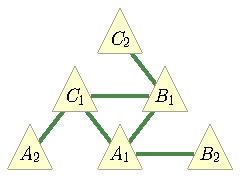
\includegraphics[scale=1]{injectiongraph222.pdf}
\caption{The injection graph corresponding to the Spiral inflation of the Triangle scenario (\cref{fig:Tri222}), wherein a pair of nodes are adjacent iff they are pairwise injectable.}\label{fig:injection222}
\end{minipage}
\hfill
\begin{minipage}[t]{0.3\linewidth}
\centering
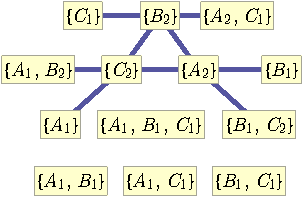
\includegraphics[scale=1]{preinjectiongraph222.pdf}
\caption{The pre-injection graph corresponding to the  Spiral inflation of the Triangle scenario (\cref{fig:Tri222}), wherein a pair of injectable sets are adjacent iff they are ancestrally independent. }\label{fig:preinjectiongraph222}
\end{minipage}
\hfill
\begin{minipage}[t]{0.3\linewidth}
\centering
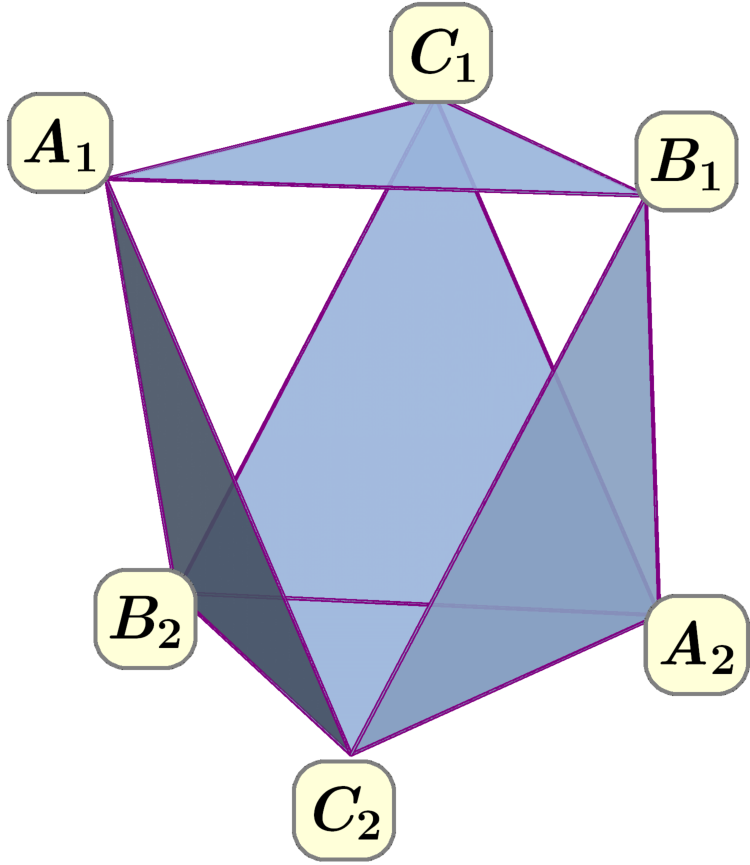
\includegraphics[scale=0.25]{simplicialcomplex.pdf}
\caption{The simplicial complex of pre-injectable sets for the  Spiral inflation of the Triangle scenario (\cref{fig:Tri222}). The 5 faces correspond to the maximal pre-injectable sets, namely $\{A_1 B_1 C_1\}$, $\{A_1 B_2 C_2\}$, $\{A_2 B_1 C_2\}$, $\{A_2 B_2 C_1\}$ and $\{A_2 B_2 C_2\}$.}\label{fig:simplicialcomplex222}
\end{minipage}
\end{figure}

From \cref{fig:injection222,fig:preinjectiongraph222}, we easily infer the injectable sets and the maximal pre-injectable sets, as well as the partition of the maximal pre-injectable sets into ancestrally independent subsets. For the Spiral example, this results in:
\begin{align}\label{eq:basicsetup222}
{\underbrace{\begin{matrix}
\, \\
\brackets{A_1},\:\brackets{B_1},\:\brackets{C_1},\\
\brackets{A_2},\:\brackets{B_2},\:\brackets{C_2},\\
\brackets{A_1 B_1},\:\brackets{A_1 C_1},\:\brackets{B_1 C_1},\\
\brackets{A_1 B_2}.\:\brackets{A_2 C_1},\:\brackets{B_1 C_2},\\
\brackets{A_1 B_1 C_1}
\end{matrix}}_{\substack{\text{injectable sets}}}}
\qquad\qquad
{\underbrace{\begin{matrix}
\brackets{A_1 B_1 C_1} \\
\brackets{A_1 B_2 C_2} \\
\brackets{B_1 C_2 A_2} \\
\brackets{C_1 A_2 B_2} \\
\brackets{A_2 B_2 C_2}
\end{matrix}}_{\substack{\text{maximal}\\\text{pre-injectable sets}}}}
\qquad
{\underbrace{\begin{matrix}
\\
\{A_1 B_2\} \aindep \{ C_2\} \\
\{B_1 C_2\} \aindep \{ A_2\} \\
\{C_1 A_2\} \aindep \{ B_2\} \\
\{A_2\} \aindep \{B_2\} \aindep \{ C_2\}
\end{matrix}}_{\substack{\text{relevant}\\\text{ancestral independences}}}}
\end{align}

Having identified the pre-injectable sets and how they partition into injectable sets, we now infer the factorization relations implied by ancestral independences, which is \cref{eq:tri222fac} in our running example. Next, we discuss the other ingredient of our systematic procedure: the marginal problem.

\subsection{The marginal problem and its solution}
\label{step:marginalsproblem}

The third step in our procedure is determining whether the given distributions on pre-injectable sets can arise as marginals of one joint distribution on all observed nodes of the inflation DAG. In general, the problem of determining whether a given family of distributions can arise as marginals of some joint distribution is known as the {\em marginal problem}\footnote{For further references and an outline of the long history of the marginal problem, see~\cite{fritz2013marginal}. An alternative account using the language of presheaves can also be found in~\cite{abramsky_contextuality_2011}.}. In order to derive causal compatibility inequalities, one must solve the closely related problem of determining necessary and sufficient \emph{constraints} that a family of marginal distributions must satisfy in order for the marginal problem to have a solution. For better clarity, we distinguish these two variants of the marginal problem as the \tblue{marginal satisfiability problem} and the \tblue{marginal constraint problem}. The generic \tblue{marginal problem} is an umbrella term referring to both types.


To specify either sort of marginal problem, one must specify the full set of variables to be considered, denoted $\bm{X}$, together with a family of subsets of $\bm{X}$, denoted $(\bm{U}_1,\ldots,\bm{U}_n)$ and called \tblue{contexts}. The family of contexts can be visualized through the simplicial complex that it generates, as illustrated in~\cref{fig:simplicialcomplex222}. A \tblue{marginal scenario} consists of a specification of contexts together with a specification of the cardinality of each variable. Every joint distribution $P_{\bm{X}}$ defines a family of marginal distributions $(P_{\bm{U}_1},\ldots,P_{\bm{U}_n})$ through marginalization,  $P_{\bm{U}_i} := \sum_{\bm{X} \setminus \bm{U}_i} P_{\bm{X}}$. The marginal problem concerns the converse inference. In the marginal satisfiability problem, a concrete family of distributions $(P_{\bm{U}_1},\ldots,P_{\bm{U}_n})$ is given, and one wants to decide whether there exists a joint distribution $\hat{P}_{\bm{X}}$ such that $P_{\bm{U}_i} = \sum_{\bm{X}\setminus\bm{U}_i} \hat{P}_{\bm{X}}$ for all $i$. In the marginal constraint problem, one seeks to find conditions on the family of distributions $(P_{\bm{U}_1},\ldots,P_{\bm{U}_n})$, considered as parameters, for when a joint distribution $\hat{P}_{\bm{X}}$ exists which reproduces these as marginals, $P_{\bm{U}_i} = \sum_{\bm{X}\setminus\bm{U}_i} \hat{P}_{\bm{X}}$ for all $i$.
 
In order for $\hat{P}_{\bm{X}}$ to exist,  distributions on different contexts must be consistent, in the sense that marginalizing $P_{\bm{U}_i}$ to the variables in $\bm{U}_i\cap\bm{U}_j$ results in the same distribution as marginalizing $P_{\bm{U}_j}$ to those variables.  
  In many cases, this is not sufficient\footnote{Depending on how the contexts intersect with one another, this \emph{may} be sufficient. A precise characterization for when this occurs has been found by~\citet{vorobev_extension_1960}.}; indeed, we have already seen examples of additional constraints, namely, the inequalities \eqref{eq:polymonogamyraw}, \eqref{eq:MIraw} and \eqref{eq:FritzF3raw} from \cref{Sec:DerivingInequalities}.
So what are the necessary and sufficient conditions? To answer this question, it helps to realize two things:
\begin{itemize}
	\item The set of possibilities for the distribution $P_{\bm{X}}$ is the convex hull of the deterministic assignments of values to $\bm{X}$ (the deterministic distributions), and 
	\item The map $P_{\bm{X}}\mapsto (P_{\bm{U}_1},\ldots,P_{\bm{U}_n})$, describing marginalization to each of the contexts in $(\bm{U}_1,\ldots,\bm{U}_n)$, is linear.
\end{itemize}
Hence the image of the set of possibilities for the distribution $P_{\bm{X}}$ under the map $P_{\bm{X}}\mapsto (P_{\bm{U}_1},\ldots,P_{\bm{U}_n})$ is exactly the convex hull of the deterministic assignments of values to $(\bm{U}_1,\ldots,\bm{U}_n)$ which are consistent where these contexts overlap. Since there are only finitely many such deterministic assignments, this convex hull is a polytope; it is called the \tblue{marginal polytope}~\cite{kahle_marginal_2010}. Together with the above equations on coinciding submarginals, the facet inequalities of this polytope solve the marginal constraint problem. The marginal satisfiability problem asks about membership in the polytope; by the above, this becomes a linear program with the joint probabilities $P_{\bm{X}}$ as the unknowns.

To write this down more concretely, it may help to write the marginal satisfiability problem thereby in the form of a generic linear program,
\begin{align}\label{eq:marginalproblemgeneric}
    \exists?\, {\bm{x} \geq \bm{0}} :\; \bm{M}\bm{x}=\bm{b}.
\end{align}
Here, the \tblue{joint distribution vector} $\bm{x}$ is the list of unknown probabilities $P_{\bm{X}}$, where the componentwise inequality $\bm{x}\geq\bm{0}$ expresses nonnegativity of probabilities. The \tblue{marginal distribution vector} $\bm{b}$ is the list of given probabilities $P_{\bm{U}_i}$, and the \tblue{marginal description matrix} $\bm{M}$ is the matrix representation of the linear map $P_{\bm{X}}\to(P_{\bm{U}_1},\ldots,P_{\bm{U}_n})$. Its entries are zeroes and ones only. In the example contexts of \cref{fig:simplicialcomplex222} with binary variables, $\bm{M}$ is a $48\times 64$ matrix, so that $\bm{M}\bm{x}=\bm{b}$ represents 48 equations and $\bm{x} \geq \bm{0}$ represents 64 inequalities. Normalization of probability for the joint distribution vector can be imposed in addition, but does not need to be, as it is a consequence of reproducing the given marginals. A single linear program can then assess whether there is a solution in $\bm{x}$ for a given marginal distribution vector $\bm{b}$. If this is not the case, then the marginal satisfiability problem has a negative answer. In our application to causal inference, this means that the original distribution has been witnessed as incompatible with the original DAG. 

Since linear programming is quite easy, probing specific distributions for compatibility for a given inflation DAG is computationally inexpensive. For instance, using the rather large Web inflation of the Triangle scenario (\cref{fig:TriFullDouble}), our numerical computations have reproduced the result of~\cite[Theorem~2.16]{fritz2012bell}, that a certain distribution considered therein is incompatible with the Triangle scenario\footnote{This distribution {\em is}, however, quantum-compatible with the Triangle scenario (\cref{sec:classicallity}).}.

In the case of the marginal constraint problem, the marginal description vector $\bm{b}$ is not given, but one rather wants to find conditions on $\bm{b}$ that hold if and only if \cref{eq:marginalproblemgeneric} has a solution. As per the above, this is a problem of \tblue{facet enumeration}\footnote{In \cref{sec:projalgorithms}, we provide an overview of techniques for facet enumeration.} for the marginal polytope. Equivalently, it is the problem of \tblue{linear quantifier elimination}\footnote{Linear quantifier elimination has already been used in causal inference for deriving entropic causal compatibility inequalities \cite{chaves2014novel,chaves2014informationinference}. In that task, however, the unknowns being eliminated are entropies on sets of variables of which one or more is latent. By contrast, the unknowns being eliminated above are all probabilities on sets of variables all of which are observed---but on the inflation DAG rather than the original DAG.} for the system of \cref{eq:marginalproblemgeneric}: one tries to find a system of linear equations and inequalities in $\bm{b}$ such that some $\bm{b}$ satisfies the system if and only if \cref{eq:marginalproblemgeneric} has a solution. There is a unique minimal system achieving this, and it consists of the consistent-submarginals equations mentioned above, together with the facet inequalities of the marginal polytope. Taken together, these form a system of linear equations and inequalities that is equivalent to \cref{eq:marginalproblemgeneric}, but does not contain any quantifiers. In our application, the consistent-submarginals equations are guaranteed to hold automatically, so that only the facet inequalities that are of interest to us.

In terms of \cref{eq:marginalproblemgeneric}, a valid inequality---such as a facet inequality of the marginal polytope---is represented by a vector of coefficients $\bm{y}$, in terms of which the inequality takes the form $\bm{y}^T\bm{b}\geq 0$ for marginal distribution vectors $\bm{b}$. That the inequality is valid for the marginal polytope means precisely that $\bm{y}^T\bm{M}\geq\bm{0}$, since the columns of $\bm{M}$ are the vertices of the polytope. The marginal satisfiability problem for given $\bm{b}$ has no solution if and only if there is a valid inequality $\bm{y}$ with $\bm{y}^T\bm{b} < 0$. For if \cref{eq:marginalproblemgeneric} has a solution $\bm{x}$, then $\bm{y}^T\bm{M}\geq \bm{0}$ and $\bm{x}\geq \bm{0}$ imply $\bm{y}^T\bm{b} = \bm{y}^T\bm{M}\bm{x} \geq 0$; the other direction is Farkas' lemma. Most linear programming tools are capable of returning such a \emph{Farkas infeasibility certificate} \cite{infeasibilitycertificates} whenever a linear program has no solution\footnote{Farkas infeasibility certificates are available, for example, in \href[pdfnewwindow]{http://docs.mosek.com/8.0/pythonapi/optimizer-task-gety.html}{\textit{Mosek}}, \href[pdfnewwindow]{https://www.gurobi.com/documentation/6.5/refman/farkasdual.html}{\textit{Gurobi}}, and \href[pdfnewwindow]{http://www-01.ibm.com/support/docview.wss?uid=swg21400058}{\textit{CPLEX}}, as well as by accessing dual variables in \href[pdfnewwindow]{http://cvxr.com/cvx/doc/basics.html\#dual-variables}{\textit{cvxr}}/\href[pdfnewwindow]{http://cvxopt.org/userguide/coneprog.html\#linear-cone-programs}{\textit{cvxopt}}.}.

Upon substituting the factorization relations of \cref{eq:preinjfactor} and deleting copy indices, any valid inequality $\bm{y}$ turns into a causal compatibility inequality. This applies both to facet inequalities of the marginal polytope, and to Farkas infeasibility certificates. In the latter case, one obtains an explicit causal compatibility inequality which witnesses the given distribution as incompatible with the given DAG. In other words, if a numerically-specified distribution is witnessed as incompatible with a DAG using the technique we have described, then with little additional numerical effort, one can also obtain a causal compatibility inequality that exhibits the incompatibility. This may have applications to problems where the facet enumeration is computationally intractable.

Summarizing, we have shown how to leverage the marginal satisfiability problem to witness causal incompatibility of particular distributions, and the marginal constraint problem to derive causal compatibility inequalities.


\subsection{A list of causal compatibility inequalities for the Triangle scenario}
\label{sec:CCineqs}


As an example of the above method, we present all of the causal compatibility inequalities that one can derive for the Triangle scenario with binary observed variables using the Spiral inflation (\cref{fig:Tri222}). The contexts for the marginal problem are the maximal pre-injectable sets of \cref{eq:basicsetup222} and \cref{fig:simplicialcomplex222}. With respect to symmetry transformations generated by permutations of the observed variables that are symmetries of the DAG and flipping the value of one variable, our facet enumeration computation shows that the marginal polytope has 64 symmetry classes of facets. Applying the factorization of probabilities according to ancestral independences per \cref{eq:preinjfactor,eq:basicsetup222} and converting into inequalities for the original DAG using \cref{maincorollary} results in 64 polynomial inequalities up to symmetry. However, there is no guarantee that each one of these inequalities is nontrivial at the level of the original DAG, where nontriviality of an inequality means that it is violated by at least one distribution. Numerically, we find that only 37 of the inequalities are indeed nontrivial, and we present these here in correlator form\footnote{A machine-readable version of this list of inequalities may be found in \cref{sec:38ineqs}.}:
\begin{align*}
\hspace{-\mathindent}\resizebox{\linewidth}{!}{\(
\begin{array}{ll}
 \text{($\#$} 1^* \text{):  } & 0\leq 1+\expec{B} \expec{C}+\expec{AB}+\expec{AC} \\
 \text{($\#$} 2 \text{):  } & 0\leq 2+\expec{A} \expec{B} \expec{C}-\expec{C} \expec{AB}-2 \expec{AC} \\
 \text{($\#$} 3^* \text{):  } & 0\leq 3+\expec{A}-\expec{B}+\expec{C}+\expec{B} \expec{C}+\expec{A} \expec{B}
   \expec{C}+\expec{AB}-\expec{C} \expec{AB}+3 \expec{AC}-\expec{B} \expec{AC} \\
 \text{($\#$} 4^* \text{):  } & 0\leq 3+\expec{A}-\expec{B}+\expec{C}+\expec{B} \expec{C}-\expec{A} \expec{B}
   \expec{C}+\expec{AB}+\expec{C} \expec{AB}+3 \expec{AC}-\expec{B} \expec{AC} \\
 \text{($\#$} 5 \text{):  } & 0\leq 3+\expec{B}-\expec{A} \expec{B}+\expec{A} \expec{C}+\expec{A} \expec{B}
   \expec{C}+\expec{AB}+\expec{C} \expec{AB}-\expec{B} \expec{AC}-2 \expec{BC} \\
 \text{($\#$} 6 \text{):  } & 0\leq 3+\expec{B}+\expec{A} \expec{C}+\expec{A} \expec{B} \expec{C}-\expec{C} \expec{AB}-2
   \expec{AC}-\expec{B} \expec{AC}-2 \expec{BC} \\
 \text{($\#$} 7 \text{):  } & 0\leq 3+\expec{B}+\expec{A} \expec{B}-\expec{A} \expec{C}-\expec{A} \expec{B}
   \expec{C}+\expec{AB}+\expec{C} \expec{AB}+\expec{B} \expec{AC}-2 \expec{BC} \\
 \text{($\#$} 8^* \text{):  } & 0\leq 3+\expec{A}+\expec{B}+\expec{A} \expec{B}+\expec{C}+\expec{A} \expec{C}+\expec{B}
   \expec{C}-\expec{A} \expec{B} \expec{C}+2 \expec{AB}+\expec{C} \expec{AB}+2 \expec{AC}+\expec{B} \expec{AC}+2 \expec{BC}+\expec{A}
   \expec{BC}-\expec{ABC} \\
 \text{($\#$} 9^* \text{):  } & 0\leq 3+\expec{A}+\expec{B}-\expec{A} \expec{B}+\expec{C}+\expec{A} \expec{C}+\expec{B}
   \expec{C}-\expec{A} \expec{B} \expec{C}+\expec{C} \expec{AB}+2 \expec{AC}+\expec{B} \expec{AC}-2 \expec{BC}-\expec{A}
   \expec{BC}+\expec{ABC} \\
 \text{($\#$} 10^* \text{):  } & 0\leq 4+2 \expec{A} \expec{B}+2 \expec{C}+2 \expec{B} \expec{C}-2 \expec{AB}+\expec{C} \expec{AB}-2
   \expec{AC}+\expec{B} \expec{AC}+\expec{A} \expec{BC}-\expec{ABC} \\
 \text{($\#$} 11^* \text{):  } & 0\leq 4-2 \expec{B}+\expec{B} \expec{C}+\expec{A} \expec{B} \expec{C}-2 \expec{AB}+\expec{C}
   \expec{AB}-\expec{B} \expec{AC}-3 \expec{BC}+\expec{ABC} \\
 \text{($\#$} 12^* \text{):  } & 0\leq 4-2 \expec{B}+2 \expec{A} \expec{C}+\expec{B} \expec{C}-\expec{A} \expec{B} \expec{C}-2
   \expec{AB}+\expec{C} \expec{AB}-2 \expec{AC}+\expec{B} \expec{AC}-3 \expec{BC}+\expec{ABC} \\
 \text{($\#$} 13^* \text{):  } & 0\leq 4-2 \expec{A} \expec{B}-2 \expec{A} \expec{C}-\expec{B} \expec{C}-\expec{A} \expec{B}
   \expec{C}+2 \expec{AB}-\expec{C} \expec{AB}-2 \expec{AC}+\expec{B} \expec{AC}+\expec{BC}+\expec{ABC} \\
 \text{($\#$} 14^* \text{):  } & 0\leq 4-2 \expec{A} \expec{B}+2 \expec{A} \expec{C}-\expec{B} \expec{C}+\expec{A} \expec{B}
   \expec{C}+2 \expec{AB}+\expec{C} \expec{AB}-2 \expec{AC}+\expec{B} \expec{AC}+\expec{BC}+\expec{ABC} \\
 \text{($\#$} 15^* \text{):  } & 0\leq 4+2 \expec{A} \expec{C}+\expec{B} \expec{C}+\expec{A} \expec{B} \expec{C}-\expec{C} \expec{AB}-2
   \expec{AC}-\expec{B} \expec{AC}+3 \expec{BC}+\expec{ABC} \\
 \text{($\#$} 16^* \text{):  } & 0\leq 4-2 \expec{B}+2 \expec{A} \expec{C}-2 \expec{AB}+\expec{C} \expec{AB}-2 \expec{AC}+\expec{B}
   \expec{AC}-2 \expec{BC}-\expec{A} \expec{BC}+\expec{ABC} \\
 \text{($\#$} 17^* \text{):  } & 0\leq 4+2 \expec{A} \expec{B}+2 \expec{A} \expec{C}+2 \expec{B} \expec{C}-2 \expec{AB}+\expec{C}
   \expec{AB}-2 \expec{AC}+\expec{B} \expec{AC}-2 \expec{BC}+\expec{A} \expec{BC}+\expec{ABC} \\
 \text{($\#$} 18 \text{):  } & 0\leq 5+\expec{A}+\expec{B}-2 \expec{A} \expec{B}+\expec{C}+\expec{B} \expec{C}+\expec{A} \expec{B}
   \expec{C}+3 \expec{AB}+\expec{C} \expec{AB}+\expec{AC}-\expec{B} \expec{AC}-4 \expec{BC} \\
 \text{($\#$} 19^* \text{):  } & 0\leq 5+\expec{A}+\expec{B}+2 \expec{A} \expec{B}+\expec{C}-2 \expec{A} \expec{C}+\expec{B}
   \expec{C}-\expec{A} \expec{B} \expec{C}+3 \expec{AB}+\expec{C} \expec{AB}-\expec{AC}+\expec{B} \expec{AC}-4 \expec{BC} \\
 \text{($\#$} 20^* \text{):  } & 0\leq 5+\expec{A}-\expec{B}-2 \expec{A} \expec{B}+\expec{C}-\expec{A} \expec{C}+\expec{B}
   \expec{C}+\expec{AB}+\expec{C} \expec{AB}+2 \expec{AC}-2 \expec{B} \expec{AC}-2 \expec{BC}-2 \expec{A} \expec{BC}-2 \expec{ABC} \\
 \text{($\#$} 21^* \text{):  } & 0\leq 5+\expec{A}+\expec{B}+\expec{C}-\expec{A} \expec{C}-\expec{B} \expec{C}-2 \expec{A} \expec{B}
   \expec{C}+\expec{AB}+2 \expec{C} \expec{AB}+2 \expec{AC}+\expec{B} \expec{AC}-2 \expec{BC}+\expec{A} \expec{BC}-\expec{ABC} \\
 \text{($\#$} 22^* \text{):  } & 0\leq 5-\expec{A}+\expec{B}-2 \expec{A} \expec{B}+\expec{C}-2 \expec{A} \expec{C}+2 \expec{B}
   \expec{C}+\expec{AB}-2 \expec{C} \expec{AB}+\expec{AC}-2 \expec{B} \expec{AC}-\expec{BC}-2 \expec{A} \expec{BC}+\expec{ABC} \\
 \text{($\#$} 23^* \text{):  } & 0\leq 5+\expec{A}+\expec{B}-\expec{A} \expec{B}+\expec{C}+2 \expec{B} \expec{C}+\expec{A} \expec{B}
   \expec{C}+2 \expec{AB}-\expec{C} \expec{AB}+\expec{AC}-2 \expec{B} \expec{AC}-\expec{BC}-2 \expec{A} \expec{BC}+\expec{ABC} \\
 \text{($\#$} 24^* \text{):  } & 0\leq 5+\expec{A}+\expec{B}-2 \expec{A} \expec{B}+\expec{C}-\expec{A} \expec{C}-\expec{B} \expec{C}-2
   \expec{A} \expec{B} \expec{C}-\expec{AB}+2 \expec{C} \expec{AB}+2 \expec{AC}+\expec{B} \expec{AC}+2 \expec{BC}-\expec{A}
   \expec{BC}+\expec{ABC} \\
 \text{($\#$} 25 \text{):  } & 0\leq 6+2 \expec{A} \expec{B}+\expec{A} \expec{C}+2 \expec{B} \expec{C}+\expec{A} \expec{B} \expec{C}-4
   \expec{AB}-2 \expec{C} \expec{AB}-3 \expec{AC}-\expec{B} \expec{AC}-2 \expec{A} \expec{BC} \\
 \text{($\#$} 26 \text{):  } & 0\leq 6-2 \expec{A}+\expec{A} \expec{B}+2 \expec{C}+\expec{A} \expec{C}+2 \expec{A} \expec{B}
   \expec{C}-5 \expec{AB}-\expec{C} \expec{AB}-3 \expec{AC}+\expec{B} \expec{AC}-2 \expec{A} \expec{BC} \\
 \text{($\#$} 27 \text{):  } & 0\leq 6+2 \expec{A} \expec{B}+2 \expec{C}+\expec{A} \expec{C}+\expec{A} \expec{B} \expec{C}-4
   \expec{AB}-2 \expec{C} \expec{AB}+3 \expec{AC}+\expec{B} \expec{AC}-2 \expec{A} \expec{BC} \\
 \text{($\#$} 28 \text{):  } & 0\leq 6+\expec{A} \expec{B}+\expec{A} \expec{C}-4 \expec{B} \expec{C}-2 \expec{A} \expec{B}
   \expec{C}+\expec{AB}+\expec{C} \expec{AB}-3 \expec{AC}-\expec{B} \expec{AC}+2 \expec{BC}-2 \expec{A} \expec{BC} \\
 \text{($\#$} 29 \text{):  } & 0\leq 6+2 \expec{B}+\expec{A} \expec{B}-2 \expec{A} \expec{C}+\expec{B} \expec{C}-2 \expec{A} \expec{B}
   \expec{C}+3 \expec{AB}+\expec{C} \expec{AB}+2 \expec{B} \expec{AC}-5 \expec{BC}+\expec{A} \expec{BC} \\
 \text{($\#$} 30 \text{):  } & 0\leq 6+2 \expec{B}-2 \expec{A} \expec{B}+4 \expec{A} \expec{C}-\expec{B} \expec{C}+\expec{A} \expec{B}
   \expec{C}+2 \expec{AB}+2 \expec{C} \expec{AB}-2 \expec{AC}+2 \expec{B} \expec{AC}+\expec{BC}+\expec{A} \expec{BC} \\
 \text{($\#$} 31 \text{):  } & 0\leq 6+\expec{A} \expec{C}+4 \expec{B} \expec{C}+\expec{A} \expec{B} \expec{C}-2 \expec{AB}-2 \expec{C}
   \expec{AB}-3 \expec{AC}-\expec{B} \expec{AC}-2 \expec{BC}-2 \expec{ABC} \\
 \text{($\#$} 32 \text{):  } & 0\leq 7+\expec{A}+\expec{B}+\expec{A} \expec{B}+\expec{C}-2 \expec{A} \expec{C}+2 \expec{B}
   \expec{C}-\expec{A} \expec{B} \expec{C}+2 \expec{AB}+3 \expec{C} \expec{AB}+\expec{AC}+2 \expec{B} \expec{AC}-3 \expec{BC}-2
   \expec{A} \expec{BC}+3 \expec{ABC} \\
 \text{($\#$} 33 \text{):  } & 0\leq 8+2 \expec{A} \expec{B}+4 \expec{A} \expec{C}-2 \expec{B} \expec{C}+2 \expec{A} \expec{B}
   \expec{C}-2 \expec{AB}-\expec{C} \expec{AB}-4 \expec{AC}+\expec{B} \expec{AC}-2 \expec{BC}-3 \expec{A} \expec{BC}-3 \expec{ABC} \\
 \text{($\#$} 34 \text{):  } & 0\leq 8+2 \expec{A}-2 \expec{C}-\expec{A} \expec{C}+2 \expec{B} \expec{C}+3 \expec{A} \expec{B}
   \expec{C}-6 \expec{AB}+\expec{C} \expec{AB}+\expec{AC}+2 \expec{B} \expec{AC}-3 \expec{A} \expec{BC}+\expec{ABC} \\
 \text{($\#$} 35 \text{):  } & 0\leq 8+2 \expec{A}+\expec{A} \expec{C}+2 \expec{B} \expec{C}+3 \expec{A} \expec{B} \expec{C}+6
   \expec{AB}-\expec{C} \expec{AB}+\expec{AC}-2 \expec{B} \expec{AC}-2 \expec{BC}-3 \expec{A} \expec{BC}+\expec{ABC} \\
 \text{($\#$} 36 \text{):  } & 0\leq 8-2 \expec{B}+2 \expec{A} \expec{B}-2 \expec{C}-\expec{B} \expec{C}-3 \expec{A} \expec{B}
   \expec{C}+3 \expec{C} \expec{AB}-6 \expec{AC}+\expec{B} \expec{AC}+\expec{BC}-2 \expec{A} \expec{BC}+\expec{ABC} \\
 \text{($\#$} 37 \text{):  } & 0\leq 8+2 \expec{B}+\expec{A} \expec{B}-2 \expec{A} \expec{C}-3 \expec{A} \expec{B}
   \expec{C}+\expec{AB}+2 \expec{C} \expec{AB}+2 \expec{AC}+3 \expec{B} \expec{AC}-6 \expec{BC}-\expec{A} \expec{BC}+\expec{ABC} \\
\end{array}
\)}
\end{align*}
A star next to the index of an inequality indicates that the inequality can also be derived by considering the possibilistic constraints per \cref{sec:TSEM}. It is likely that this list of inequalities contains redundant ones; a minimal list would be one where, for every inequality, there is a distribution that violates it while satisfying all of the others. 


\subsection{Causal compatibility inequalities via Hardy-type inferences from logical tautologies}\label{sec:TSEM}

Enumerating all the facets of the marginal polytope is computationally feasible only for small examples. But our method transforms \emph{every} inequality that bounds the marginal polytope into a causal compatibility inequality. We now present a general approach for deriving a special type of such inequalities very quickly.

In the literature on Bell inequalities, it has been noticed that incompatibility with the Bell DAG can sometimes be witnessed by merely looking at which joint outcomes have zero probability and which ones have nonzero probability. In other words, instead of considering the \emph{probability} of an outcome, the inconsistency of some marginal distributions can be evident from considering only the \emph{possibility} or \emph{impossibility} of each outcome. This insight is originally due to~\citet{L.Hardy:PRL:1665}, and versions of Bell's theorem that are based on the violation of such \tblue{possibilistic constraints} are known as \tblue{Hardy-type paradoxes}~\cite{Garuccio95,CabelloHardyInequality,Braun08,Mancinska14,LSW}; a partial classification of these can be found in~\cite{Mansfield2012}. The method that we describe in the second half of this section can be used to compute a complete classification of possibilistic constraints for \emph{any} marginal problem.

Possibilistic constraints follow from a consideration of {\em logical relations} that can hold among deterministic assignments to the observed variables. Such logical constraints can also be leveraged to derive probabilistic constraints instead of possibilistic ones, as shown in~\cite{Pitowsky1989,Ghirardi08}. This results in a partial solution to any given (probabilistic) marginal problem. Essentially, we solve a possibilistic marginal problem \cite{Mansfield2012}, then upgrade the possibilistic inequalities into probabilistic inequalities, resulting in a set of probabilistic inequalities whose cumulative satisfaction is a necessary but insufficient condition for satisfying the corresponding probabilistic marginal problem. We now demonstrate how to systematically derive all inequalities of this type.

We have already provided a simple example of a Hardy-type argument in \cref{example:noWdist}, in the logic used to demonstrate that the marginal distributions of \cref{W4,W1,W5} cannot arise from a joint distribution. For our present purposes, it is useful to recast that argument into a new but manifestly equivalent form. First, for the distribution in question, we have
\begin{align} 
\begin{split}\label{WWs}
&A_2 = 1 \:\implies\: C_1 = 0,\\
&B_2 = 1 \:\implies\: A_1 = 0,\\
&C_2  = 1 \:\implies\: B_1  = 0,\\
\text{Never}  &\quad A_1  = 0\,\text{ and }\, B_1  = 0\,\text{ and }\, C_1  = 0.
\end{split}
\end{align}
From the last constraint one infers that at least one of $A_1$, $B_1$ and $C_1$ must be 1, which from the three other constraints implies that at least one of $A_2$, $B_2$ and $C_2$ must be 0, so that it is not the case that all of $A_2$, $B_2$ and $C_2$ are 1.  Thus~\cref{WWs} implies
\begin{align} \label{consequent2}
\text{Never}  \quad &A_2  = 1\,\text{ and }\, B_2  = 1\,\text{ and }\, C_2  = 1.
\end{align}
However, the Spiral inflation (\cref{fig:Tri222v2}) is such that $A_2$, $B_2$, and $C_2$ have no common ancestor and consequently the distribution on the pre-injectable set $\{A_2 B_2 C_2\}$ also has full support, which contradicts \cref{consequent2}.

We are here interested in recasting the argument in a manner amenable to systematic generalization. This is done as follows. We work in a marginal scenario where the contexts are $\{A_2 B_2 C_2\}$, $\{A_2 C_1\}$, $\{B_2 A_1\}$, $\{C_2 B_1\}$, and  $\{A_1 B_1 C_1\}$, and all variables are binary. The first step of the argument is to note that\footnote{Here, $\land$, $\lor$ and $\lnot$ denote conjunction, disjunction and negation respectively.}
\begin{align}\begin{split}\label{tautology1}
&\lnot [A_2 \eql 1, C_1 \eql 1] \bigwedge \lnot [B_2 \eql 1, A_1 \eql 1] \bigwedge \lnot [C_2 \eql 1, B_1 \eql 1] \bigwedge \lnot [A_1 \eql 0, B_1 \eql 0, C_1 \eql 0]\\
 &\qquad\implies
\lnot [A_2 \eql 1, B_2 \eql 1, C_2 \eql 1].
\end{split}\end{align}
is a logical tautology for binary variables. It can be understood as a constraint on marginal {\em deterministic assignments}, which can be thought of as a logical counterpart of a linear inequality bounding the marginal polytope. The second and final step of the argument notes that the given marginal distributions are such that the antecedent is always true, while the consequent is sometimes false.

To see how to translate this into a constraint on marginal {\em distributions}, we rewrite \cref{tautology1} in its contrapositive form,
\begin{align}\begin{split}\label{tautology2}
&[\mgreen{A_2 \eql 1} , \mgreen{B_2 \eql 1} , \mgreen{C_2 \eql 1}]  \implies [\mgreen{A_2 \eql 1}, C_1 \eql 1] \lor  [\mgreen{B_2 \eql 1}, A_1 \eql 1] \lor  [\mgreen{C_2 \eql 1}, B_1 \eql 1] \lor  [A_1 \eql 0, B_1 \eql 0, C_1 \eql 0].
\end{split}\end{align}
Next, we note that if a logical tautology can be expressed as
\begin{align}\label{eq:inference}
    E_0 \implies E_1 \lor \ldots \lor E_n,
\end{align}
then by applying the union bound---which asserts that the probability of at least one of a set of events occuring is no greater than the sum of the probabilities of each event occuring---one obtains
\begin{align}\label{eq:possinference}
\p{E_0}\leq \sum\limits_{j=1}^n{\p{E_j}}.
\end{align}
Applying this to \cref{tautology2} in particular yields
\begin{align}\label{eq:F3rawweak}
P_{A_2 B_2 C_2}\parens{\mgreen{1} \mgreen{1} \mgreen{1}} \leq P_{A_1 B_2}\parens{1 \mgreen{1 }}+P_{ B_1 C_2}\parens{ 1 \mgreen{1}}+P_{A_2 C_1}\parens{\mgreen{1 } 1}+P_{A_1 B_1 C_1}\parens{0 0 0},
\end{align}
which is a constraint on the marginal {\em distributions}.
 
This inequality allows one to demonstrate the incompatibility of the marginal distributions of \cref{W4,W1,W5} with the Spiral inflation just as easily as one can with the tautology of \cref{tautology1}.  It suffices to note that the given distribution and causal structure imply that the left-hand side has nonzero probability (which corresponds to the consequent of \cref{tautology1} being sometimes false) while every term on the right-hand side has zero probability (which corresponds to the antecedent of \cref{tautology1} being always true).
But, of course, the inequality can witness many other incompatibilities in addition to this one.

As another example, consider the marginal problem where the variables are $A$, $B$ and $C$, with each being binary, and the contexts are the pairs $\{AB\}$, $\{AC\}$, and $\{BC\}$.  
The following tautology provides a constraint on marginal deterministic assignments:\footnote{This is a tautology since $E \land F  \implies  E \land F \land (G \lor \lnot G) = (E \land F \land G) \lor (E\land F \land \lnot G) \implies (E \land G) \lor (F \land \lnot G)$.}
\begin{align}\label{GHZtautology}
 \bracks{\mgreen{A \eql 0}, \mgreen{C \eql 0}} \implies \bracks{\mgreen{A \eql 0}, B \eql 0} \lor \bracks{B \eql 1, \mgreen{C \eql 0}}.
\end{align}
Applying the union bound, one obtains a constraint on marginal distributions,\footnote{This inequality is equivalent to \cref{eq:polymonogamyraw}.}
\[
P_{AC}(\mgreen{0 0}) \leq P_{AB}(\mgreen{0} 0) + P_{BC}(1 \mgreen{0}).
\]

In this section, we seek to determine, for any marginal scenario, the set of \emph{all} inequalities that can be derived in this manner.  We do so by \tblue{enumerating} the full set of tautologies of the form \cref{tautology1,GHZtautology}. This boils down to solving the possibilistic version of the marginal constraint problem.

We outline the general procedure using the marginal scenario of~\cref{fig:simplicialcomplex222}, where the full set of variables is $\{ A_1, A_2, B_1, B_2, C_1, C_2\}$ and the contexts are $\{A_1 B_1 C_1\}$, $\{A_1 B_2 C_2\}$, $\{A_2 B_1 C_2\}$, $\{A_2 B_2 C_1\}$ and $\{A_2 B_2 C_2\}$, pursuant to \cref{eq:basicsetup222}.
As before, we will express the constraints on marginal deterministic assignments as logical implications with
a valuation (assignment of outcomes) on one of the contexts as the \tblue{antecedent} and a disjunction over valuations on contexts as the \tblue{consequent}. In the following, we explain how to generate \emph{all} such implications which are tight in the sense that the consequent is minimal, i.e., involves as few terms as possible in the disjunction. 

First, we fix the antecedent by choosing some context and a joint valuation of its variables. In order to generate all constraints on marginal deterministic assignments, one will have to perform this procedure for \emph{every} context as the antecedent and every choice of valuation thereon. For the sake of concreteness, we take the above example with $\bracks{\mgreen{A_2 \eql 1}, \mgreen{B_2 \eql 1}, \mgreen{C_2 \eql 1}}$ as the antecedent.  
Each logical implication we consider is required to have the property that any variable that appears in both the antecendent and the consequent must be given the same value in both. 

To formally determine all valid consequents, we consider two hypergraphs, or equivalently 0/1-matrices with rows that enumerate the vertices and columns that correspond to hyperedges, so that the $1$'s indicate the incidences between vertices and hyperedges.

Each vertex in the first hypergraph corresponds to a valuation on some particular context. 
Each hyperedge corresponds to a possible joint valuations of \emph{all} the variables. Such a hyperedge contains a vertex if the valuation represented by the hyperedge is an extension of the valuation represented by the vertex. For example the hyperedge $\bracks{A_1 \eql 0, \mgreen{A_2 \eql 1}, B_1 \eql 0, \mgreen{B_2 \eql 1}, C_1 \eql 1, \mgreen{C_2 \eql 1}}$ contains the vertex $\bracks{A_1 \eql 0,  \mgreen{B_2 \eql 1}, \mgreen{C_2 \eql 1}}$. In our example following \cref{fig:simplicialcomplex222}, this initial hypergraph has $5\cdot 2^3 = 40$ vertices and $2^6 = 64$ hyperedges. In 0/1-matrix notation, this first hypergraph is precisely the marginal description matrix $\bm{M}$ introduced near \cref{eq:marginalproblemgeneric}.

The second hypergraph is a subhypergraph of the first one. We delete from the first hypergraph all vertices and hyperedges which contradict the outcomes supposed by the antecedent. For example, the vertex $\bracks{\mgreen{A_2 \eql 1}, \mred{B_2 \eql 0}, C_1 \eql 1}$ contradicts the antecedent $\bracks{\mgreen{A_2 \eql 1}, \mgreen{B_2 \eql 1}, \mgreen{C_2 \eql 0}}$. We also delete the vertex corresponding to the antecedent itself. In our example, this second hypergraph has $2^3 + 3\cdot 2^1 = 14$ vertices and $2^3 = 8$ hyperedges.

All valid (minimal) consequents are (minimal) \tblue{transversals} of this latter hypergraph. A transversal is a set of vertices which has the property that it intersects every hyperedge in at least one vertex. In order to get implications which are as tight as possible, it is sufficient to enumerate only the minimal transversals. Doing so is a well-studied problem in computer science with various natural reformulations and for which manifold algorithms have been developed~\cite{eiter_dualization_2008}.

In our example, it is not hard to check that the consequent of
\begin{align}\begin{split}\label{eq:F3implicationform}
	\bracks{\mgreen{A_2 \eql 1}, \mgreen{B_2 \eql 1}, \mgreen{C_2 \eql 1}}  \quad\Longrightarrow\quad & \bracks{A_1 \eql 1, \mgreen{B_2 \eql 1}, \mgreen{C_2 \eql 1}} \lor \bracks{\mgreen{A_2 \eql 1}, B_1 \eql 1, \mgreen{C_2 \eql 1}} \\
	 \lor & \bracks{\mgreen{A_2 \eql 1}, \mgreen{B_2 \eql 1}, C_1 \eql 1} \lor \bracks{A_1 \eql 0, B_1 \eql 0, C_1 \eql 0}
\end{split}\end{align}
is such a minimal transversal: every assignment of values to all variables which extends the assignment on the left-hand side satisfies at least one of the terms on the right, but this ceases to hold as soon as one removes any one term on the right. 

We convert these implications into inequalities in the usual way via the union bound (i.e., replacing ``$\Rightarrow$'' by ``$\leq$'' at the level of probabilities and the disjunctions by sums). For example \cref{eq:F3implicationform} translates into the constraint on marginal distributions
\begin{align}\label{eq:F3rawprobform}
    P_{A_2 B_2 C_2}\parens{\mgreen{1} \mgreen{1} \mgreen{1}} \leq P_{A_1 B_2 C_2}\parens{1 \mgreen{1 1}}+P_{A_2 B_1 C_2}\parens{\mgreen{1} 1 \mgreen{1}}+P_{A_2 B_2 C_1}\parens{\mgreen{1 1} 1} + P_{A_1 B_1 C_1}\parens{0 0 0}.
\end{align}
This inequality is a strengthening of \cref{eq:F3rawweak}.  \cref{eq:F3rawprobform} was used earlier in this article as the starting point of our third example of how to derive a causal compatibility inequality for the Triangle scenario, \cref{eq:FritzF3raw}. Because \cref{eq:F3implicationform} is the progenitor of this inequality, it can be thought of as the progenitor of the causal compatibility inequality that one derives from it, namely, \cref{eq:FritzF3}.  

Inequalities on marginal distributions that one derives from hypergraph transversals are generally weaker than those that result from a complete solution of the marginal problem. Nevertheless, many Bell inequalities are of this form, the CHSH inequality among them \cite{Ghirardi08}.  So it seems that this method is still sufficiently powerful to generate plenty of interesting inequalities. At the same time, it should be significantly easier to perform in practice than the full-fledged facet enumeration, even if one does it for every possible antecedent.

In conclusion, facet enumeration is the preferred method for deriving inequalities for the marginal problem whenever it is computationally tractable; but whenever it is not, then enumerating hypergraph transversals presents a good alternative.


\section{Further prospects for the inflation technique}\label{sec:otherprospects}

\cref{mainlemma} and \cref{maincorollary} state that any causal inference technique on an inflation DAG $G'$ can be transferred to the original DAG $G$. In the previous section, we have found that even extremely weak techniques on $G'$---namely the existence of a joint distribution plus ancestral independences---can lead to significant and new results for causal inference on $G$. In the following two subsections, we consider two additional possibilities for constraints that might be exploited in this way to enhance the power of inflation further.

\subsection{Using \textit{d}-separation relations on the inflation DAG}\label{sec:fulldsep}

In \cref{sec:ineqs}, we considered causal inference by studying the existence of a joint distribution on observed nodes of the inflation DAG, and then making use of the ancestral independences to factorize the joint distributions on the pre-injectable sets into those on the injectable sets.

It is natural to wonder whether one can sometimes make use of facts about the causal structure that go beyond ancestral independences.  It is standard practice, when deriving compatibility conditions for a DAG, to make use of arbitrary $d$-separation relations among variables: if, in a given DAG, $\bm{X}$ and $\bm{Y}$ are $d$-separated\footnote{The notion of $d$-separation is treated at length in~\cite{pearl2009causality,studeny2005probabilistic,WoodSpekkens,pusey2014gdag}, so we elect not to review it here.} by $\bm{Z}$, then a distribution is compatible with that DAG only if it satisfies the conditional independence relation $\bm{X}\indep\bm{Y}|\bm{Z}$. For $\bm{Z} = \emptyset$, this specializes to ancestral independence of $\bm{X}$ and $\bm{Y}$. Thus it is natural to ask: can the inflation technique also sensibly make use of other $d$-separation relations among sets of observed variables?



Every conditional independence relation $\bm{X}\indep\bm{Y}|\bm{Z}$ can be expressed as a polynomial equation in terms of probabilities: while it is most commonly written as $P_{\bm{X}\bm{Y}|\bm{Z}}(\bm{x}\bm{y}|\bm{z})=P_{\bm{X}|\bm{Z}}(\bm{x}|\bm{z})P_{\bm{Y}|\bm{Z}}(\bm{y}|\bm{z})$ for all $\bm{x}$, $\bm{y}$, and $\bm{z}$, it can also be written in terms of unconditional probabilities, where it takes the form
\[
\forall{\bm{x} \bm{y} \bm{z}}: \p[\bm{X}\bm{Y}\bm{Z}]{\bm{x}\bm{y}\bm{z}}\p[\bm{Z}]{\bm{z}}=\p[\bm{X}\bm{Z}]{\bm{x}\bm{z}}\p[\bm{Y}\bm{Z}]{\bm{y}\bm{z}}
\]
Such a nonlinear constraint can be incorporated as a further restriction on the joint distributions compatible with the inflation DAG, supplementing the basic constraints of nonnegativity of probabilities for the joint distribution of the observed variables and the constraints implied by ancestral independences.

For example, in the Spiral inflation of the Triangle scenario~(\cref{fig:Tri222}), $A_1$ and $C_2$ are $d$-separated by $\{A_2 B_2\}$, in addition to being ancestrally independent. Hence one can try to incorporate the constraint that 
\begin{align}\label{nonlinearequality}
\forall{a_1 a_2 b_2 c_2}: \p[A_1 A_2 B_2 C_2]{a_1 a_2 b_2 c_2}\p[A_2 B_2]{a_2 b_2}=\p[A_1 A_2 B_2]{a_1 a_2 b_2}\p[A_2 B_2 C_2]{a_2 b_2 c_2}
\end{align}
 Every probability that appears in such an equation, though not defined on an injectable set, can still be expressed as a marginal of the joint distribution of all observed variables.  For instance, we can express $\pfunc{A_2 B_2}$ as
\begin{align}
\forall{a_2 b_2}:\;\p[A_2 B_2]{a_2 b_2} = \sum\nolimits_{a_1 b_1 c_1 c_2}\p[A_1 A_2 B_1 B_2 C_1 C_2]{a_1 a_2 b_1 b_2 c_1 c_2}.
\end{align}
Upon substituting such relations into~\cref{nonlinearequality}, one obtains a system of polynomial equations and inequalities in terms of the observed joint probabilities.  We can then proceed with quantifier elimination as we did before, eliminating the unknowns $\p[A_1 A_2 B_1 B_2 C_1 C_2]{a_1 a_2 b_1 b_2 c_1 c_2}$ from this system. The additional difficulty now is that some of the equations are nonlinear. This idea even applies to some ancestral independences between sets that are not pre-injectable: for example, $A_1 A_2 B_2 \indep C_2$ is also guaranteed in the Spiral inflation of the Triangle scenario~(\cref{fig:Tri222}), and results in a polynomial equation closely related to \cref{nonlinearequality}.

Many modern computer algebra systems have functions capable of tackling nonlinear quantifier elimination symbolically\footnote{For example \textit{Mathematica$^{_{\textit{\tiny\texttrademark}}}$}'s \href[pdfnewwindow]{http://reference.wolfram.com/language/ref/Resolve.html}{\texttt{Resolve}} command, \textit{Redlog}'s \href[pdfnewwindow]{http://www.redlog.eu/documentation/reals/rlqe.php}{\texttt{rlposqe}}, or \textit{Maple$^{_{\textit{\tiny\texttrademark}}}$}'s \href[pdfnewwindow]{http://maplesoft.com/support/help/Maple/view.aspx?path=RegularChains/SemiAlgebraicSetTools/RepresentingQuantifierFreeFormula}{\texttt{RepresentingQuantifierFreeFormula}}.}. 
Currently, however, it is generally not practical to perform nonlinear quantifier elimination on large polynomial systems with many unknowns to be eliminated. It may help to exploit results on the concrete algebraic-geometric structure of these particular systems~\cite{garcia_bayesian_2005}. 

If one is seeking merely to assess the compatibility of a {\em given} distribution with the causal structure, then one can avoid the quantifier elimination problem and simply try and solve an existence problem: after substituting the values that the given distribution prescribes for the outcomes on pre-injectable sets into the polynomial system in terms of the unknown global joint probabilities, one must only determine whether that system has a solution. Most computer algebra systems can resolve such \emph{satisfiability} questions quite easily\footnote{For example \textit{Mathematica$^{_{\textit{\tiny\texttrademark}}}$}'s \href[pdfnewwindow]{http://reference.wolfram.com/language/Experimental/ref/ExistsRealQ.html}{\texttt{Reduce\`{}ExistsRealQ}} function. Specialized satisfiability software such as SMT-LIB's \href[pdfnewwindow]{http://smtlib.cs.uiowa.edu/solvers.shtml}{\texttt{check-sat}} \cite{BarFT-SMTLIB} are particularly apt for this purpose.}.

It is also possible to use a mixed strategy of linear and nonlinear quantifier elimination, such as \citet{ChavesPolynomial} advocates. The explicit results of~\cite{ChavesPolynomial} are directly causal implications of the \emph{original} DAG, achieved by applying a mixed quantifier elimination strategy. Perhaps further causal compatibility inequalities will be derivable by applying such a mixed quantifier elimination strategy to inflation DAGs.

\subsection{Using copy-index equivalence on the inflation DAG}\label{Sec:copyindexequivalence}

By the definition of an inflation model (\cref{def:inflat}), if two variables in the inflation DAG $G'$ are copy-index-equivalent, $A_i \sim A_j$, then each depends on its parents in the same fashion as $A$ depends on its parents in the original DAG $G$. By transitivity, also $A_i$ and $A_j$ have the same dependence on their parents.  Formally, from $A_i \sim A$ and \cref{eq:funcdependences}, we infer that $\pfunc{A_i| \Pa[G']{A_i}}=\pfunc{A|\Pa[G]{A}}$, and similarly $\pfunc{A_j| \Pa[G']{A_j}}=\pfunc{A|\Pa[G]{A}}$, which results in
\begin{align}\label{copyindexequivalence}
\pfunc{A_i| \Pa[G']{A_i}}=\pfunc{A_j|\Pa[G']{A_j}}.
 \end{align}
By the definition of inflation, the ancestral subgraphs of $A_i$ and $A_j$ are identical, and equations like \cref{copyindexequivalence} also hold for all their ancestors. We conclude that also the marginal distributions of $A_i$ and $A_j$ must be equal, $\pfunc{A_i}=\pfunc{A_j}$.
More generally, it may be possible to find pairs of contexts in $G'$ of any size such that constraints of the form of~\cref{copyindexequivalence} imply that the marginal distributions on these two contexts must be equal. 

For example, consider the pair of contexts $\brackets{A_1 A_2 B_1}$ and $\brackets{A_1 A_2 B_2}$ for the marginal scenario defined by the Spiral inflation (\cref{fig:Tri222}). Neither of these two contexts is an injectable set.  Nonetheless, because of~\cref{copyindexequivalence}, we can conclude that their marginal distributions coincide in any inflation model,
\begin{align}\label{CIEconsequence}
\forall{a a' b}:\;\p[A_1 A_2 B_1]{a a' b} = \p[A_1 A_2 B_2]{a a' b}.
\end{align}
We can also conclude that in the inflation model these marginal distributions satisfy  $P_{A_1 A_2 B_1}=P_{A_2 A_1 B_2}$---where now the order of $A_1$ and $A_2$ is opposite on the two sides of the equation---or equivalently, 
\begin{align}\label{CIEconsequence2}
\forall{a a' b}:\;\p[A_1 A_2 B_1]{a a' b} = \p[A_1 A_2 B_2]{a' a b}.
\end{align}
These constraints entail that $P_{A_1 A_2 B_2}$ must be symmetric under exchange of $A_1$ and $A_2$, which in itself is another equation of the type above.

Parameters such as $\p[A_1 A_2 B_1]{a_1 a_2 b}$, $\p[A_1 A_2 B_2]{a_1 a_2 b}$ and $\p[A_1 A_2]{a_1 a_2}$ can each be expressed as sums of the unknowns $\p[A_1 A_2 B_1 B_2 C_1 C_2]{a_1 a_2 b_1 b_2 c_1 c_2}$, so that relations such as \cref{CIEconsequence,CIEconsequence2} each constitute an additional equation that can be added to the system of equations and inequalities that constitute the starting point of the satisfiability problem (if one is seeking to test the compatibility of a given distribution with the inflation DAG) or the quantifier elimination problem (if one is seeking to derive causal compatibility inequalities for the inflation DAG).  If any such additional constraints yield stronger constraints at the level of the inflation DAG, then they may translate into stronger constraints at the level of the original DAG.

The general problem of finding pairs of marginal contexts in the inflation DAG for which relations of copy-index-equivalence imply equality of the marginal distributions, and the conditions under which such equalities may yield tighter inequalities, are discussed in \cref{sec:coincidingdetails}.


\subsection{Causal inference in quantum theory and in generalized probabilistic theories}
\label{sec:classicallity}

Recent work has sought to explore quantum generalizations of the notion of a causal model, termed {\em quantum causal models} \cite{leifer2013conditionalstates,pusey2014gdag,BeyondBellII,Chaves2015infoquantum,ried2015quantum}. We now sketch the definition used in~\cite{pusey2014gdag}.
The causal structures are still represented by DAGs, but now in a quantum causal model the outgoing edges of latent nodes are different from the other ones: they carry physical systems, meaning that each such edge must be labelled by a Hilbert space. Each latent node takes all its incoming information---represented by its observed parent variables together with the incoming physical systems---and turns it into outgoing information via a quantum channel. Similarly, an observed node takes all its incoming information and applies a joint measurement on its incoming physical systems as well as some classical information processing resulting in an outcome for its associated variable. Root variables can be thought of as settings or preparation procedures, while terminal nodes often represent the outcomes of measurements that are used in an experiment on quantum systems. In most cases that are of interest to quantum foundations, this complicated definition of quantum causal model can be formulated in an equivalent form that does not require a distinction of two kinds of edges~\cite{BeyondBellII}.

A quantum causal model is still ultimately in the service of explaining joint distributions over classical variables. The joint distribution of these variables is the only experimental data with which one can confront a given quantum causal model. The basic problem of causal inference for quantum causal models, therefore, concerns the compatibility of a joint distribution of observed classical variables with a given DAG, where the model supplementing the DAG is allowed to be quantum. If this happens, we say that the distribution is {\em quantumly compatible} with the DAG.  
 

One motivation for studying quantum causal models is that they offer a new perspective on an old  problem in the quantum foundations: that of establishing precisely which of the principles of classical physics must be abandoned in quantum physics. It was noticed by~\citet{fritz2012bell} and~\citet{WoodSpekkens} that Bell's theorem~\cite{bell1966lhvm} states that there are distributions on observed nodes of the Bell DAG that are quantumly compatible but not classically compatible with the DAG. Moreover, these distributions cannot be explained by \emph{any} causal structure while complying with the additional principle that conditional independences should not be fine-tuned~\cite{WoodSpekkens}, i.e.,~while demanding that any observed conditional independence should be accounted for by the DAG. These results suggest that quantum theory is perhaps best understood as revising our notions of the nature of unobserved entities, how one represents causal dependencies thereon and incomplete knowledge thereof, while 
nonetheless {\em preserving} the spirit of causality and the principle of no fine-tuning~\cite{leifer2013conditionalstates,Spekkens2015paradigm,henson2011ontic}.

Another motivation for studying quantum causal models is a practical one.  Violations of Bell inequalities have  been shown to constitute resources for information processing \cite{NoSigPolytope,scarani2012device,BancalDIApproach}. Hence it seems plausible that the existence of distributions on other DAGs that are quantumly compatible but not classically compatible may have similar applications to information processing. 
For example, it has been shown that in addition to the Bell scenario, such a quantum-classical separation also exists 
in the bilocality scenario \cite{BilocalCorrelations} and the Triangle scenario~\cite{fritz2012bell}, and it is likely that many more DAGs with this property will be found.  The hope is that on any DAG supporting a quantum-classical separation, some of the separating distributions may constitute a resource for information processing. 

So for both foundational and practical reasons, there is good reason to find examples of DAGs that exhibit a quantum-classical separation.
However, this is by no means an easy task.
The set of distributions that are quantumly compatible with a given DAG is quite hard to separate from the set of distributions that are classically compatible with that DAG~\cite{pusey2014gdag,fritz2012bell}. For example, both the classical and quantum sets respect the conditional independence relations among observed nodes that are implied by the $d$-separation relations of the DAG~\cite{pusey2014gdag}, and entropic inequalities are only of very limited use~\cite{chaves2012entropic,fritz2012bell}. We hope that the inflation technique will provide better tools for finding such separations.


In addition to quantum generalizations of causal models, one can define generalizations for other operational theories that are neither classical nor quantum~\cite{pusey2014gdag,BeyondBellII}.
Such generalizations are formalized using the framework of {\em generalized probabilistic theories} (GPTs) \cite{Barnum2012GPT,Janotta2014GPT}, which is sufficiently general to describe any operational theory that makes statistical predictions about the outcomes of experiments and passes some basic sanity checks.  Some constraints on compatibility can be proven to be \emph{theory-independent} in that they apply not only to classical and quantum causal models, but to any kind of generalized probabilistic causal model~\cite{pusey2014gdag}. For example, the classically-valid conditional independence relations implied between observed variables in a DAG are all also valid in the GPT framework.
Another example is the entropic monogamy inequality \cref{eq:monogomyofcorrelations}, which was proven in \cite{pusey2014gdag} to be GPT valid as well. These kinds of constraints are of interest because they clarify what any conceivable theory of physics must satisfy on a given causal structure. 

The essential element in deriving such constraints is to only make reference to the observed nodes, as done in~\cite{pusey2014gdag}. In fact, we now understand the argument of~\cite{pusey2014gdag} to be an instance of the inflation technique. Nonetheless, we have seen that the inflation technique often yields inequalities that hold for the {\em classical} notion of compatibility, while having quantum and GPT violations, such as the Bell inequalities of \cref{example:noPR} of \cref{subsec:witnessingincompat} and \cref{sec:Bellscenarios}. In fact, inflation can be used to derive inequalities with quantum violations for the Triangle scenario as well \cite{TC2016trianglequantum}.

So what distinguishes applications of the inflation technique that yield inequalities for GPT compatibility from those that yield inequalities for classical compatibility?   The distinction rests on a structural feature of the inflation DAG:




\begin{definition}
In $G'\in\inflations{G}$, an \tblue{inflationary fan-out} is a latent node that has two or more children that are copy-index equivalent.  
\end{definition}

 The Web and Spiral inflations of the Triangle scenario, depicted in \cref{fig:TriFullDouble} and \cref{fig:Tri222} respectively,
contain one or more inflationary fan-outs, as does the inflation of the Bell DAG that is depicted in \cref{fig:BellDagCopy1}.  On the other hand, the simplest inflation of the Triangle scenario that we consider in this article, the Cut inflation depicted in \cref{fig:simplestinflation}, does not contain any inflationary fan-outs.

Our main observation is that if one uses an inflation DAG without an inflationary fan-out, then the resulting inequalities derived by the inflation technique will all be GPT valid. In other words, one can only hope to detect a GPT-classical separation if one uses an inflation DAG that \emph{has} at least one inflationary fan-out. We now explain the intuition for why this is the case. 
In an inflation model, the copy-index-equivalent children of an inflationary fan-out causally depend on it in precisely the same way as their counterparts in the original DAG do. For example, this dependence may be such that these two children are exact \emph{copies} of the inflationary fan-out node. So when one tries to write down a quantum or GPT version of our notion of inflation model, one quickly runs into trouble: in quantum theory, the {\em no-broadcasting theorem} shows that such duplication is impossible in a strong sense~\cite{NoCloningQuantum1996}, and an analogous theorem holds for GPTs~\cite{NoCloningGeneral2006}. This is why in the presence of an inflationary fan-out, one cannot expect our inequalities to hold in the quantum or GPT case, which is consistent with the fact that they often do have quantum and GPT violations.

On the other hand, for any inflation DAG that does not contain an inflationary fan-out, the notion of inflation model generalizes to the quantum case: one equips every latent node in $G'$ with the same quantum channel that the corresponding node in $G$ is labelled by, while possibly discarding the outgoing systems which leave the node on those edges that do not appear in $G'$. For observed nodes, one can likewise use the exact same data as on $G$. That these prescriptions make sense crucially rests on the assumption that $G'$ is an inflation of $G$, so that the ancestries of any node in $G'$ mirrors the ancestry of the corresponding node in $G$ perfectly. Hence for inflation DAGs $G'$ without inflationary fan-outs, we have quantum analogues of \cref{mainlemma} and \cref{maincorollary}. The problem of quantum causal inference on $G$ therefore translates into the corresponding problem on $G'$, and any constraint that we can derive on $G'$ translates back to $G$. In particular, our \cref{example:noGHZ,example:polytriangle,example:entropic} also hold for quantum causal inference: perfect correlation is also quantumly incompatible with the Triangle scenario, and the inequalities \cref{eq:polymonogamy,eq:monogomyofcorrelations} have no quantum violations. All of the exact same statements apply likewise in the GPT case.


In the remainder of this section, we discuss the relation between the quantum and the GPT case. Since quantum theory is a particular generalized probabilistic theory, quantum compatibility trivially implies GPT compatibility. Through the work of Tsirelson \cite{Tsirelson1980} and \citet{PROriginal}, it is known that the converse is not true: the Bell scenario manifests a GPT-quantum separation.  The identification of distributions witnessing this difference, and the derivation of constraints on quantum compatibility with GPT violations, has been a focus of much foundational research in recent years. Traditionally, the foundational question has always been: why does quantum theory predict correlations that are {\em stronger} than one would expect classically?  But now there is a new question being asked: why does quantum theory only allow correlations that are {\em weaker} than those predicted by other GPTs?  There has been some interesting progress in identifying physical principles that can pick out the precise correlations that are exhibited by quantum theory \cite{PopescuReviewNatureComm,ScaraniML,Rohrlich2014,InfoCausArXiv,LONatureComm,LOExploring,EPNBody,barnum2014interference,AlmostQuantum}.  Further opportunities for identifying such principles would be useful.  This motivates the problem of classifying DAGs into those which have a quantum-classical separation, those which have a GPT-quantum separation and those which have both. Similarly, one can try to classify causal compatibility \emph{inequalities} into those which are GPT-valid, those which are GPT-violable-but-quantum-valid, and those which are quantum-violable. 

It may be possible to generalize the inflation technique to derive inequalities that can witness a GPT-quantum separation by finding a restricted notion of quantum causal model on inflation DAGs \emph{with} inflationary fan-outs that would not apply to the GPT case.
In quantum theory, there {\em are} linear maps that can achieve broadcasting~\cite{Coecke2011}, but these are not completely positive. Thus if one uses these to define the inflation of a quantum causal model, then some of the observed joint probabilities in the inflation DAG may end up being negative.  Such inflations might still be useful as a mathematical tool for ultimately deriving causal compatibility inequalities on the original DAG, but one would need to proceed differently from the way we have proceeded in this article: whereas we have assumed that all joint outcomes on the inflation DAG have nonnegative probability, one could not impose such a constraint for the type of quantum inflation just described.  Instead, one could only demand nonnegativity for marginal distributions of collections of variables that do not include the children of an inflationary fan-out. The inflation DAG in such cases would not be physically realistic, but one could still interpret it as describing multiple different {\em counterfactual} scenarios within which the causal dependencies are the same.

An analysis along these lines has already been carried out successfully in the derivation of entropic inequalities that capture quantum compatibility. Namely, \citet{Chaves2015infoquantum} consider conditioning an observed variable on a ``setting'' variable, a structure that we would describe as an inflation DAG containing inflationary fan-outs. \citet{Chaves2015infoquantum} then take pains to avoid talking about a global joint distribution in any of the entropic inequalities they apply to this structure, 
precisely as we would want to do in constructing inequalities on our inflation DAG. In this way, they successfully derive entropic inequalities for quantum compatibility. So far, no inequalities polynomial in the probabilities have been derived using this method.





\section{Conclusions}

We have described the \emph{inflation technique} for doing causal inference with latent variables.

We have shown how many existing techniques for witnessing incompatibility and for deriving causal compatibility inequalities can be enhanced by the inflation technique, independently of whether these pertain to entropic quantities, correlators or probabilities. The computational difficulty of achieving this enhancement depends on the seed technique.  We summarize the computational difficulty of the approaches that we have considered in~\cref{table:difficulties}. While this focuses on deriving inequalities, the same table applies \emph{mutatis mutandis} to the satisfiability problem. 

\begin{table}[ht]
\centering
\caption{
A comparison of different approaches for deriving constraints on compatibility at the level of the inflation DAG, which then translate into constraints on compatibility at the level of the original DAG.
}
\begin{tabularx}{\linewidth}{ |c|RlL|c| } 
\toprule
Input from causal structure & General problem & $\to$ & Standard algorithm(s) & Difficulty \\
\midrule
\midrule
	\multirow{ 2}{*}{\parbox{5cm}{\centering Only ancestral independences among the observed variables}}  & Facet enumeration of mar-\linebreak ginal polytope (\cref{step:marginalsproblem})  & $\to$ & see \cref{sec:projalgorithms} & Hard \\\cline{2-5}

	& Finding possibilistic constraints \linebreak by identifying hypergraph transversals (\cref{sec:TSEM}) & $\to$ & see~\citet{eiter_dualization_2008} & Very easy \\

\hline
\parbox{5cm}{All $d$-separation conditions on the observed variables (\cref{sec:fulldsep})} & Real quantifier elimination & $\to$ & Cylindrical algebraic decomposition~\cite{ChavesPolynomial} & Very hard \\

\hline
\parbox{5cm}{Ancestral independences among the observed variables + copy-index equivalences (\cref{sec:coincidingdetails})} & Linear quantifier elimination & $\to$ & Fourier-Motzkin elimination~\cite{fordan1999projection,DantzigEaves,Bastrakov2015,BalasProjectionCone,Jones2008}, \linebreak Equality set projection \cite{JonesThesis2005,jones2004equality} & Hard \\

\bottomrule
\end{tabularx}
\label{table:difficulties}
\end{table}

Especially in \cref{sec:ineqs}, we have focused on one particular seed technique: the existence of a joint distribution on all observed nodes together with ancestral independences. We have shown how a complete or partial solution of the marginal problem for the pre-injectable sets of the inflation DAG can be leveraged to obtain criteria for causal compatibility, both at the level of witnessing particular distributions as incompatible and deriving causal compatibility inequalities. These inequalities are polynomial in the joint probabilities of the observed variables. They are capable of exhibiting the incompatibility of the W-type distribution with the Triangle scenario, while entropic techniques cannot, so that our polynomial inequalities are stronger than entropic inequalities in at least some cases (see \cref{example:noWdist} of \cref{subsec:witnessingincompat}). As far as we can tell, our inequalities are not related to the nonlinear causal compatibility inequalities which have been derived specifically to constrain classical networks \cite{TavakoliStarNetworks,RossetNetworks,TavakoliNoncyclicNetworks}, nor to the nonlinear inequalities which account for interventions to a given causal structure \cite{kang2007polynomialconstraints,steeg2011relaxation}.

We have shown that \emph{some} of the causal compatibility inequalities we derive by the inflation technique are necessary conditions not only for compatibility with a classical causal model, but also for compatibility with a causal model in {\em any} generalized probabilistic theory, which includes quantum causal models as a special case. It would be enlightening to understand the general extent to which our polynomial inequalities for a given DAG can be violated by a distribution arising in a quantum causal model for that DAG. A variety of techniques exist for estimating the amount by which a Bell inequality \cite{NPA2008Long,I3322NPA1} is violated in quantum theory, but even finding a quantum violation of one of our \emph{polynomial} inequalities for causal structures other than the Bell scenario presents a new task for which we currently lack a systematic approach. Nevertheless, we know that there exists a difference between classical and quantum also beyond Bell scenarios~\cite[Theorem~2.16]{fritz2012bell}, and we hope that our polynomial inequalities will perform better in probing this separation than entropic inequalities do~\cite{pusey2014gdag,Chaves2015infoquantum}. Along similar lines, we also hope that it is possible to modify our methods to derive inequalities that may witness the separation between quantum and general probabilistic causal models in DAGs other than the Bell scenario. This may eventually provide an alternative approach to understanding the Tsirelson bound \cite{Brunner2013Bell}.


A single causal structure has an unlimited number of potential inflations. Selecting a good inflation from which strong polynomial inequalities can be derived is an interesting challenge. To this end, it would be desirable to understand how particular features of the original causal structure are exposed when different nodes in the DAG are duplicated. By isolating which features are exposed in each inflation, we could conceivably quantify the utility for causal inference of each inflation. In so doing, we might find that inflation DAGs beyond a certain level of variable duplication need not be considered. The multiplicity beyond which further inflation is irrelevant may be related to the maximum degree of those polynomials which tightly characterize a causal scenario. Presently, however, it is not clear how to upper bound either number, or whether finite upper bounds can even be expected.


Causal compatibility inequalities are, by definition, merely {\em necessary} conditions for compatibility. Depending on what kind of causal inference methods one uses at the level of an inflation DAG $G'$, one may or may not obtain sufficient conditions. An interesting question is: if one only uses the existence of a joint distribution and ancestral independences at the level of $G'$, then does one obtain sufficient conditions as $G'$ varies? In other words: if a given distribution is such that for every $G'$, the marginal problem of \cref{sec:ineqs} is solvable, then is the distribution compatible with the original DAG? This occurs for the Bell scenario, where it is enough to consider only one particular inflation (\cref{sec:Bellscenarios}). Some evidence against sufficiency in the general case is that we have not seen a way to use the inflation technique to rederive Pearl's instrumental inequality.






\begin{acknowledgments}
E.W.~would like to thank Rafael Chaves and T.C. Fraser for suggestions which have improved this manuscript. T.F.~would like to thank Nihat Ay and Guido Mont\'ufar for discussion and references. This research was supported in part by Perimeter Institute for Theoretical Physics. Research at Perimeter Institute is supported by the Government of Canada through the Department of Innovation, Science and Economic Development Canada and by the Province of Ontario through the Ministry of Research, Innovation and Science.
\end{acknowledgments}


\appendix
\numberwithin{equation}{section}
\let\stdsection\section
\renewcommand{\section}{\clearpage\stdsection} % new page for each section






\section{Algorithms for solving the marginal constraint problem}\label{sec:projalgorithms}

By solving the marginal constraint problem, what we mean is to determine all the facets of the marginal polytope for a given marginal scenario. Since the vertices of this polytope are precisely the deterministic assignments of values to all variables, which are easy to enumerate, solving the marginal problem is an instance of a \tblue{facet enumeration problem}: given the vertices of a convex polytope, determine its facets. This is a well-studied problem in combinatorial optimization for which a variety of algorithms are available~\cite{avis_convexhull_2015}. 

A generic facet enumeration problem takes a matrix $\bm{V}\in\mathbb{R}^{d\times n}$, which lists the vertices as its columns, and asks for an inequality description of the set of vectors $\bm{b}\in\mathbb{R}^d$ that can be written as a convex combination of the vertices using weights $\bm{x}\in\mathbb{R}^n$ that are nonnegative and normalized,
\begin{align}
	\label{projsimplex}
	\left\{\: \bm{b}\in\mathbb{R}^d \quad\bigg|\quad \exists \bm{x}\in\mathbb{R}^n:\; \bm{b} = \bm{V}\bm{x} ,\;\; \bm{x}\geq \bm{0},\;\; {{\sum_i}{x_i}}=1 \:\right\}.
\end{align}
To solve the marginal problem one uses the marginal description matrix introduced in \cref{step:marginalsproblem} as the input to the facet enumeration algorithm, i.e. $\bm{V}=\bm{M}$, see \cref{eq:marginalproblemgeneric}.

The oldest-known method for facet enumeration relies on \tblue{linear quantifier elimination} in the form of Fourier-Motzkin (FM) elimination~\cite{fordan1999projection,DantzigEaves}. This refers to the fact that one starts with the system $\bm{b}= \bm{V}\bm{x}$, $\bm{x}\geq \bm{0}$ and ${{\sum_i}{x_i}}=1$, which is the half-space representation of a convex polytope (a simplex), and then one needs to project onto $\bm{b}$-space by \emph{eliminating} the variables $\bm{x}$ to which the existential \emph{quantifier} $\exists \bm{x}$ refers. The Fourier-Motzkin algorithm is a particular method for performing this quantifier elimination one variable at a time; when applied to~\cref{projsimplex}, it is equivalent to the \emph{double description method}~\cite{DantzigEaves,Fukuda1996}. Linear quantifier elimination routines are available in many software tools\footnote{For example \textit{MATLAB$^{_{\textit{\tiny\texttrademark}}}$}'s \href[pdfnewwindow]{http://people.ee.ethz.ch/~mpt/2/docs/refguide/mpt/@polytope/projection.html}{\texttt{MPT2}}/\href[pdfnewwindow]{http://ellipsoids.googlecode.com/svn-history/r2740/branches/issue_119_vrozova/tbxmanager/toolboxes/mpt/3.0.14/all/mpt3-3_0_14/mpt/modules/geometry/sets/@Polyhedron/projection.m}{\texttt{MPT3}}, \textit{Maxima}'s \href[pdfnewwindow]{http://maxima.sourceforge.net/docs/manual/de/maxima_75.html}{\texttt{fourier\_elim}}, \textit{lrs}'s \href[pdfnewwindow]{http://cgm.cs.mcgill.ca/~avis/C/lrslib/USERGUIDE.html\#fourier}{\texttt{fourier}}, or \textit{Maple$^{_{\textit{\tiny\texttrademark}}}$}'s (v17+) \href[pdfnewwindow]{http://www.maplesoft.com/support/help/maple/view.aspx?path=RegularChains/SemiAlgebraicSetTools/LinearSolve}{\texttt{LinearSolve}} and \href[pdfnewwindow]{http://www.maplesoft.com/support/help/Maple/view.aspx?path=RegularChains/SemiAlgebraicSetTools/Projection}{\texttt{Projection}}. The efficiency of most of these software tools, however, drops off markedly when the dimension of the final projection is much smaller than the initial space of the inequalities. Fast facet enumeration aided by Chernikov rules \cite{Shapot2012,Bastrakov2015} is implemented in \href[pdfnewwindow]{https://www.inf.ethz.ch/personal/fukudak/cdd_home/}{\textit{cdd}},
\href[pdfnewwindow]{http://comopt.ifi.uni-heidelberg.de/software/PORTA/}{\textit{PORTA}}, \href[pdfnewwindow]{http://sbastrakov.github.io/qskeleton/}{\textit{qskeleton}}
, and \href[pdfnewwindow]{http://www.uic.unn.ru/~zny/skeleton/}{\textit{skeleton}}. In the authors experience \href[pdfnewwindow]{http://www.uic.unn.ru/~zny/skeleton/}{\textit{skeleton}} seemed to be the most efficient. Additionally, the package \href[pdfnewwindow]{https://polymake.org/doku.php/researchdata/polymakeilp}{\textit{polymake}} offers multiple algorithms as options for computing convex hulls.}. The authors found it convenient to custom-code a linear quantifier elimination routine in \textit{Mathematica$^{_{\textit{\tiny\texttrademark}}}$}.

Other algorithms for facet enumeration that are not based on linear quantifier elimination include the following. \emph{Lexicographic reverse search} (LRS)~\cite{Avis2000lrs} explores the entire polytope by repeatedly pivoting from one facet to an adjacent one, and is implemented in~\href[pdfnewwindow]{http://cgm.cs.mcgill.ca/~avis/C/lrslib/USERGUIDE.html#Installation\%20Section}{\texttt{lrs}}. Equality Set Projection (ESP)~\cite{jones2004equality,JonesThesis2005} is also based on pivoting from facet to facet, though its implementation is less stable\footnote{ESP  \cite{jones2004equality,JonesThesis2005,Jones2008} is supported by \href[pdfnewwindow]{http://people.ee.ethz.ch/~mpt/2/docs/refguide/mpt/@polytope/projection.html}{\texttt{MPT2}} but not \href[pdfnewwindow]{http://people.ee.ethz.ch/~mpt/3/}{\texttt{MPT3}}, and by the (undocumented) option of \href[pdfnewwindow]{https://github.com/tulip-control/polytope/blob/master/polytope/polytope.py\#L1412}{projection} in the \href[pdfnewwindow]{https://pypi.python.org/pypi/polytope}{\textit{polytope}} (v0.1.2 2016-07-13) python module.}. These algorithms could be interesting to use in practice, since each pivoting step churns out a new facet; by contrast, Fourier-Motzkin type algorithms only generate the entire list of facets at once, after all the quantifiers have been eliminated one by one.

It may also be possible to exploit special features of marginal polytopes in order to facilitate their facet enumeration, such as their high degree of symmetry: permuting the outcomes of each variable maps the polytope to itself, which already generates a sizeable symmetry group, and oftentimes there are additional symmetries given by permuting some of the variables. This simplifies the problem of facet enumeration~\cite{bremner_symmetries_2009,Schurmann2013}, and it may be interesting to apply dedicated software\footnote{Such as \href[pdfnewwindow]{http://comopt.ifi.uni-heidelberg.de/software/PANDA/}{\textit{PANDA}}, \href[pdfnewwindow]{http://mathieudutour.altervista.org/Polyhedral/}{\textit{Polyhedral}}, or \href[pdfnewwindow]{http://www.math.uni-rostock.de/~rehn/software/sympol.html}{\textit{SymPol}}. The authors found \textit{SymPol} to be rather effective for some small test problems, using the options ``\texttt{./sympol -a --cdd}".} to the facet enumeration problem of marginal polytopes~\cite{Kaibel2010,rehn_tools_2012,panda_2015}.







\section{Constraints on marginal distributions from copy-index equivalence relations}\label{sec:coincidingdetails}

In \cref{copyindexequivalence}, we noted that every copy of a variable in an inflation model has the same probabilistic dependence on its parents as every other copy. It followed that for certain pairs of marginal contexts, the marginal distributions in any inflation model are necessarily equal. We now describe how to identify such pairs of contexts. 


Given $\bm{U},\bm{V}\subseteq\nodes{G'}$ in an inflation DAG $G'$, let us say that a map $\varphi:\bm{U}\to\bm{V}$ is a \tblue{copy isomorphism} if it is a graph isomorphism\footnote{A graph isomorphism is a bijective map between the nodes of one graph and the nodes of another, such that both the map and its inverse take edges to edges.} between $\subgraph{\bm{U}}$ and $\subgraph{\bm{V}}$ such that $\varphi(X)\sim X$ for all $X\in\bm{U}$, meaning that $\varphi$ maps every node $X\in\bm{U}$ to a node $\varphi(X)\in\bm{V}$ that is equivalent to $X$ under dropping the copy-index.

Furthermore, we say that a copy isomorphism $\varphi : \bm{U}\to\bm{V}$ is an \tblue{inflationary isomorphism} whenever it can be extended to a copy isomorphism on the ancestral subgraphs, $\Phi : \An{\bm{U}}\to\An{\bm{V}}$. 
A copy isomorphism $\Phi: \An{\bm{U}}\to\An{\bm{V}}$ defines an inflationary isomorphism $\varphi:\bm{U}\to\bm{V}$ if and only if $\Phi(\bm{U}) = \bm{V}$.
So in practice, one can either start with $\varphi : \bm{U}\to\bm{V}$ and try to extend it to $\Phi : \An{\bm{U}}\to\An{\bm{V}}$, or start with such a $\Phi$ and see whether it maps $\bm{U}$ to $\bm{V}$ and thereby restricts to a $\varphi$.

For given $\bm{U}$ and $\bm{V}$, a sufficient condition for equality of their marginal distributions in an inflation model is that there exists an inflationary isomorphism between them.  Because $\bm{U}$ and $\bm{V}$ might themselves contain several variables that are copy-index equivalent (recall the examples of \cref{Sec:copyindexequivalence}), equating the distribution $P_{\bm{U}}$ with the distribution $P_{\bm{V}}$ in an unambiguous fashion requires one to specify a correspondence between the variables that make up $\bm{U}$ and those that make up $\bm{V}$. This is exactly the data provided by the inflationary isomorphism $\varphi$.  This result is summarized in the following lemma.


\begin{lemma}
Let $G'$ be an inflation of $G$, and let $\bm{U},\bm{V}\subseteq\nodes{G'}$. Then every inflationary isomorphism $\varphi:\bm{U}\to\bm{V}$ induces an equality $P_{\bm{U}} = P_{\bm{V}}$ for inflation models, where the variables in $\bm{U}$ are identified with those in $\bm{V}$ according to $\varphi$.
\label[lemma]{lem:coincide}
\end{lemma}

This applies in particular when $\bm{V} = \bm{U}$, in which case the statement is that the distribution $P_{\bm{U}}$ is invariant under permuting the variables according to $\varphi$.

\cref{lem:coincide} is best illustrated by returning to our example from \cref{Sec:copyindexequivalence} 
which considered the Spiral inflation of~\cref{fig:Tri222} and the pair of contexts $\bm{U} = \{ A_1 A_2 B_1\}$ and $\bm{V} =\{ A_1 A_2 B_2\}$. The map 
\begin{align}\label{copyisomorph}
	\varphi \: : \: A_1 \mapsto A_1,\qquad A_2\mapsto A_2,\qquad B_1\mapsto B_2
\end{align}
is a copy isomorphism between $\bm{U}$ and $\bm{V}$
because it trivially implements a graph isomorphism (both subgraphs are edgeless), and it maps each variable in $\bm{U}$ to a variable in $\bm{V}$ that is copy-index equivalent. There is a unique choice to extend $\varphi$ to a copy isomorphism $\Phi:\An{\bm{U}}\to\An{\bm{V}}$, namely, by extending~\cref{copyisomorph} to the ancestors via
\begin{align}
\Phi \: : \: X_1\mapsto X_1,\qquad Y_1\mapsto Y_1, \qquad Y_2 \mapsto Y_2, \qquad Z_1 \mapsto Z_2,
\end{align}
which is again a copy isomorphism. 
Therefore $\varphi$ is indeed an inflationary isomorphism. From \cref{lem:coincide}, we then conclude that any inflation model satisfies $P_{A_1 A_2 B_1} = P_{A_1 A_2 B_2}$.

Similarly, the map 
\begin{align}\label{copyisomorph2}
	\varphi' \: : \: A_1 \mapsto A_2,\qquad A_2\mapsto A_1,\qquad B_1\mapsto B_2
\end{align}
is easily verified to be a copy isomorphism between $\subgraph{\bm{U}}$ and $\subgraph{\bm{V}}$, and there is again a unique choice to extend $\varphi'$ to a copy isomorphism $\Phi':\ansubgraph{\bm{U}}\to\ansubgraph{\bm{V}}$, by extending~\cref{copyisomorph2} with
\begin{align}
\Phi' \: : \: X_1\mapsto X_1,\qquad Y_1\mapsto Y_2, \qquad Y_2 \mapsto Y_1, \qquad Z_1 \mapsto Z_2,
\end{align}
so that $\varphi'$ is verified to be an inflationary isomorphism. From \cref{lem:coincide}, we then conclude that any inflation model also satisfies $P_{A_1 A_2 B_1} = P_{A_2 A_1 B_2}$.  (And this in turn implies that for the context $\{A_1 A_2\}$, the marginal distribution satisfies $P_{A_1 A_2} = P_{A_2 A_1}$.)


\begin{figure}[b]
    \centering
    \begin{minipage}[t]{0.2\linewidth}      \centering
    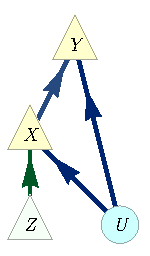
\includegraphics[scale=1]{ISorigDAG.pdf}
    \caption{The instrumental scenario of \citet{pearl1995instrumental}.}
    \label{fig:ISorigDAG}
    \end{minipage}\hfill
    \begin{minipage}[t]{0.3\linewidth}      \centering
    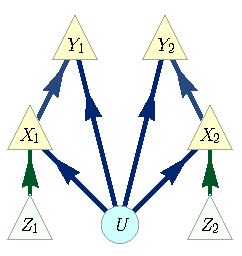
\includegraphics[scale=1]{IScopyDAG.pdf}
    \caption{An inflation DAG of the instrumental scenario which illustrates why coinciding ancestral subgraphs doesn't necessarily imply coinciding marginal distributions.}
    \label{fig:IScopyDAG}
    \end{minipage}\hfill    
    \begin{minipage}[t]{0.3\linewidth}      \centering
    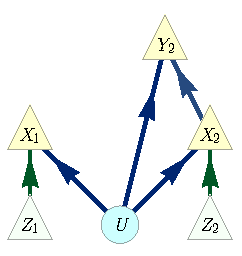
\includegraphics[scale=1]{ISancestorDAG.pdf}
    \caption{The ancestral subgraph of \cref{fig:IScopyDAG} for either $\{X_1 Y_2 Z_1\}$ or $\{X_1 Y_2 Z_2\}$.}
    \label{fig:ancestralsubgraphnotenough}
    \end{minipage}
\end{figure}

In order to avoid any possibility of confusion, we emphasize that it is not a plain copy isomorphism between the subgraphs of $\bm{U}$ and $\bm{V}$ themselves which results in coinciding marginal distributions, nor a copy isomorphism between the ancestral subgraphs of $\bm{U}$ and $\bm{V}$. It is rather an inflationary isomorphism between the subgraphs, i.e., a copy isomorphism between the ancestral subgraphs that restricts to a copy isomorphism between the subgraphs. To see why a copy isomorphism between ancestral subgraphs {\em by itself} may not be sufficient for deriving equality of marginal distributions, we offer the following example. Take as the original DAG the instrumental scenario of \citet{pearl1995instrumental}, and consider the inflation depicted in \cref{fig:IScopyDAG}.  Consider the pair of contexts $\bm{U} = \{ X_1 Y_2 Z_1\}$ and $\bm{V}= \{ X_1 Y_2 Z_2\}$ on the inflation DAG. Since $\subgraph{\bm{U}}$ and $\subgraph{\bm{V}}$ are not isomorphic, there is no copy isomorphism between the two. On the other hand, 
the ancestral subgraphs are both given by the DAG of~\cref{fig:ancestralsubgraphnotenough}, so that the identity map is a copy isomorphism between $\ansubgraph{X_1 Y_2 Z_1}$ and $\ansubgraph{X_1 Y_2 Z_2}$.

One can try to make use of \cref{lem:coincide} when deriving polynomial inequalities with inflation via solving the marginal problem, by imposing the resulting equation $P_{\bm{U}} = P_{\bm{V}}$ as an additional constraint for every inflationary isomorphism $\varphi : \bm{U}\to\bm{V}$ between sets of observed nodes. This is advantageous to speed up to the linear quantifier elimination, since one can solve each of the resulting equations for one of the unknown joint probabilities and thereby eliminate that probability directly without Fourier-Motzkin elimination. Moreover, one could hope that these additional equations also result in tighter constraints on the marginal problem, which would in turn yielder tighter causal compatibility inequalities. Our computations have so far not revealed any example of such a tightening.

In some cases, this lack of impact can be explained as follows.
Suppose that $\varphi:\bm{U}\to\bm{V}$ is an inflationary isomorphism 
which is not just the restriction of a copy isomorphism between the ancestral subgraphs, but even the restriction of a copy automorphism 
$\Phi':G'\to G'$ of the entire inflation DAG onto itself; in particular, this assumption implies that $\Phi'$ also restricts to a copy isomorphism $\Phi:\An{\bm{U}}\to\An{\bm{V}}$ between the ancestral subgraphs. In this case, the irrelevance of the additional constraint $P_{\bm{U}} = P_{\bm{V}}$ to the marginal problem for inflation models can be explained by the following argument. 

Suppose that some joint distribution $P_{\obsnodes{G'}}$ solves the unconstrained marginal problem, i.e.,~without requiring $P_{\bm{U}} = P_{\bm{V}}$. Now apply $\Phi'$ to the variables in $P_{\obsnodes{G'}}$, switching the variables around, to generate a new distribution $P'_{\obsnodes{G'}}:=P_{\Phi'(\obsnodes{G'})}$. Because the set of marginal distributions that arise from inflation models is invariant under this switching of variables, we conclude that $P'$ is also a solution to the unconstrained marginal problem. Taking the uniform mixture of $P$ and $P'$ is therefore still a solution of the unconstrained marginal problem. But this uniform mixture also satisfies the supplementary constraint $P_{\bm{U}} = P_{\bm{V}}$. Hence the supplementary constraint is satisfiable whenever the unconstrained marginal problem is solvable, which makes adding the constraint irrelevant.

This argument does not apply when the inflationary isomorphism $\varphi:\bm{U}\to\bm{V}$ cannot be extended to a copy automorphism of the entire inflation DAG. It also does not apply if one uses $d$-separation conditions beyond ancestral independence on the inflation DAG as additional constraints (\cref{sec:fulldsep}), because in this case the set of compatible distributions is not necessarily convex.  In either of these cases, it is unclear whether or not constraints arising from copy-index equivalence could yield tighter inequalities. 



\section{Using the inflation technique to certify a DAG as ``interesting"\label{sec:interestingproof}}

By considering all possible $d$-separation conditions implied by a given DAG, one can infer the set of all conditional independence (CI) relations that must hold in any joint distribution over the observed variables that is compatible with the given DAG. In the presence of latent nodes, satisfying the CI relations among observed variables 
is generally not sufficient for compatibility with the DAG. \citet{pusey2014gdag} were concerned with identifying the \tblue{interesting} DAGs, by which they mean precisely those DAGs that exhibit a discrepancy between the set of observed distributions genuinely compatible with it and the set of observed distributions that merely satisfy its observed CI relations.

\citet{pusey2014gdag} derived necessary criteria on the structure of a DAG in order for it to be interesting, and they conjectured that their criteria may also be sufficient. As evidence in favour of this conjecture, they enumerated all possible DAGs with no more than six nodes satisfying their criteria, resulting in 
only 21 equivalence classes of potentially interesting DAGs.
Of those 21, they further proved that 18 were unambiguously interesting by writing down explicit distributions which are incompatible despite satisfying the observed CI relations. Incompatibility was certified by means of entropic inequalities. 

That left three classes of DAGs  as \emph{potentially} interesting. For each of these, \citet{pusey2014gdag} derived all Shannon-type entropic inequalities in two different ways, once by accounting for non-observed CI relations (that is, CI relations that do not refer exclusively to observed variables) and once without. The existence of \emph{novel} Shannon-type inequalities upon accounting for non-observed CI relations is evidence for the DAG being interesting. The only loophole is that perhaps those novel Shannon-type inequalities are actually non-novel non-Shannon-type inequalities implied by the observed CI relations alone \cite{pusey2014gdag}. 

One way to close this loophole would be to show that the novel Shannon-type inequalities imply constraints beyond some inner approximation to the genuine entropy cone absent non-observed CI relations, perhaps along the lines of~\cite{weilenmann2016entropic}. Another is to use causal compatibility inequalities beyond entropic inequalities to identify some CI-respecting but incompatible distributions. \citet{pianaar2016interesting} accomplished precisely this, and should be credited with the original insight to explicitly consider the different values that an observed root variable may take. In the following, we demonstrate how the inflation technique can be used for this purpose. So far, we have only considered one of the three enigmatic causal structures, namely,~\cref{fig:GDAG15}.

\begin{figure}[b]
\centering
\begin{minipage}[t]{0.4\linewidth}
\centering
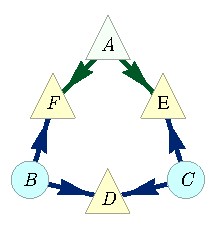
\includegraphics[scale=1]{scen15DAGV2.pdf}
\caption{DAG \#15 in Ref. \cite{pusey2014gdag}.}\label{fig:GDAG15}
\end{minipage}
\hfill
\begin{minipage}[t]{0.5\linewidth}
\centering
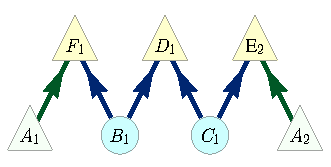
\includegraphics[scale=1]{scen15InflationDAGV2.pdf}
\caption{A useful inflation of \cref{fig:GDAG15}.}\label{fig:Inflated15}
\end{minipage}
\end{figure}

The following representative causal compatibility inequalities for the DAG of~\cref{fig:GDAG15} follow from the inflation technique applied to causal compatibility inequalities for the inflation DAG of \cref{fig:Inflated15}, where the latter are obtained from Hardy-type tautologies as described in \cref{sec:TSEM}:
\begin{align}
\p[A]{0} \p[A D E]{0 0 0} \leq {\p[A E]{0 0} \p[A F]{0 0}  + \p[A]{0} \p[A D F]{0 0 1}}, \\
\p[A]{0}\p[A D E]{1 0 0} \leq {\p[A E]{1 0} \p[A F]{0 0} + \p[A]{1} \p[A D F]{0 0 1}}.
\label{eq:DAG15ineqs}
\end{align}
For example, the second inequality may be explicitly derived as follows. A Hardy-type tautology on the variables of the inflation DAG implies the following constraint on marginals:
\begin{align}\label{eq:hardyforpienaar}
     \p[A_1 A_2 D E_2]{0100} \leq \p[A_1 A_2 E_2 F_1]{0100} + \p[A_1 A_2 D F_1]{0101} .
\end{align}
Applying factorization as per the ancestral independence relations of the inflation DAG, we obtain 
\begin{align}
 \p[A_1]{0} \p[A_2 D E_2]{100} \leq \p[A_2 E_2]{10} \p[A_1 F_1]{00} + \p[A_2]{1} \p[A_1 D F_1]{001},   
\end{align}
and finally translating this into a causal compatibility inequality on the original DAG using \cref{maincorollary}, we obtain \cref{eq:DAG15ineqs}. 
 
In \citet{pianaar2016interesting}, it was shown that the following distribution, which is easily verified to satisfy the CI relations among the observed variables of \cref{fig:GDAG15}, namely, $A\indep D$ and $E\indep F | A$~\cite{pusey2014gdag}, is nonetheless incompatible with \cref{fig:GDAG15}:
\begin{align}\label{eq:pienaardistro}
	P^{\text{Pien}}_{A D E F}:=\frac{[0000]+[0101]+[1000]+[1110]}{4},\quad\text{i.e.}\quad P^{\text{Pien}}_{A D E F}(a d e f):=\begin{cases}\tfrac{1}{4}&\text{if }  a\cdot d = e \text{ and }  (a \oplus 1)\cdot d = f, \\ 0&\text{otherwise}.\end{cases}
\end{align}

It is easily verified that this distribution violates the causal compatibility inequality of~\cref{eq:DAG15ineqs}.  It is in this sense that the inflation technique can show that the DAG of \cref{fig:GDAG15} is interesting. 

There is a different way to see that this distribution is not compatible with~\cref{eq:DAG15ineqs} using our results from the main text.  First, any marginal distribution on $DEF$ that is compatible with the DAG of \cref{fig:GDAG15} is necessarily also compatible the Triangle scenario, with $D$, $E$ and $F$ as observed variables.
Second, the marginal distribution $P^{\text{Pien}}_{D E F}$ is incompatible with the Triangle scenario, since it violates inequality \#8 of~\cref{sec:CCineqs}.  This is the same inequality which rejects the W-distribution of~\cref{eq:wdistribution1}.
Like the W-distribution, the distribution $P^{\text{Pien}}$
 not only satisfies all Shannon-type entropic inequalities pertinent to~\cref{fig:GDAG15}, but lies within an inner approximation to the genuine entropy cone for that scenario\footnote{This is due to Weilenmann and Colbeck (personal communication).}. In other words, there exists a distribution with the same joint and marginal entropies as  $P^{\text{Pien}}$ which \emph{is} compatible with \cref{fig:GDAG15}.

Finally, it may be worth noting that the inflation of~\cref{fig:Inflated15} is precisely the ``bilocality scenario'' investigated by~\citet{BilocalCorrelations}.  Therefore, the inflation technique permits us to translate every causal compatibility inequality for the bilocality scenario into a causal compatibility inequality for the DAG of~\cref{fig:GDAG15}.






\section{The copy lemma and non-Shannon type entropic inequalities}\label{sec:NonShannon}

As it turns out, the inflation technique is also useful outside of the problem of causal inference. As we argue in the following, inflation is secretly what underlies the \tblue{Copy Lemma} in the derivation of non-Shannon type entropic inequalities~\cite[Chapter~15]{yeung_network_2008}. The following formulation of the Copy Lemma is the one of \citet{kaced_equivalence_2013}.

\begin{lemma}
	Let $A$, $B$ and $C$ be random variables with distribution $P_{ABC}$. Then there exists a fourth random variable $A'$ and joint distribution $P_{AA'BC}$ such that:
	\begin{enumerate}
		\item $P_{AB} = P_{A'B}$,
		\item $A' \indep AC \:|\: B$.
	\label{copylemma}
	\end{enumerate}
\end{lemma}

The proof via inflation is as follows.
\begin{proof}
Every joint distribution $P_{ABC}$ is compatible with a DAG of the form of~\cref{fig:beforecopy}.  This follows from the fact that one may take $X$ to be any \tblue{sufficient statistic} for the joint variable $(A,C)$ given $B$, such as $X := (A,B,C)$.  Next, we consider the inflation of \cref{fig:beforecopy} depicted in~\cref{fig:aftercopy}. The maximal injectable sets are $\{ A_1 B_1 C_1\}$ and $\{A_2 B_1\}$.  By \cref{mainlemma}, because $P_{ABC}$ is assumed to be compatible with~\cref{fig:beforecopy}, it follows that the family of marginals $\{ P_{A_1 B_1 C_1}, P_{A_2 B_1}\}$, where $P_{A_1 B_1 C_1}:= P_{A B C}$ and $P_{A_2 B_1} := P_{AB}$, is compatible with the inflation of~\cref{fig:aftercopy}. The resulting joint distribution $P_{A_1 A_2 B_1 C_1}$ has marginals $P_{A_1 B_1}= P_{A_2 B_1} =P_{AB}$ and satisfies the conditional independence relation $A_2 \indep A_1 C_1 \:|\: B_1$, since $A_2$ is $d$-separated from $A_1 C_1$ by $B_1$ in \cref{fig:aftercopy}.
\end{proof}

While it is also not hard to write down the distribution constructed in the proof explicitly as $P_{A_1 A_2 B_1 C_1} := P_{A_1 B_1 C_1} P_{A_2 B_1} P_{B_1}^{-1}$~\cite[Lemma~15.8]{yeung_network_2008}, the fact that one can rederive it using the inflation technique is significant.  For one, all the non-Shannon type inequalities derived by \citet{zeger_2011_nonshannon} are obtained by applying some Shannon-type inequality to the distribution that is implied to exist by the Copy Lemma.  Our result shows, therefore, that one can understand these non-Shannon type inequalities for a DAG as arising from Shannon-type inequalities applied to an inflation DAG.  Indeed, it may be that the inflation technique may be a more general-purpose tool for deriving non-Shannon-type entropic inequalities.  A natural direction for future research is to explore whether more sophisticated applications of the inflation technique might result  in \emph{new} examples of such inequalities. 


\begin{figure}[H]
\centering
\begin{minipage}[t]{0.4\linewidth}
\centering
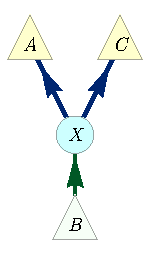
\includegraphics[scale=1]{shannonNOcopyV1.pdf}
\caption{A causal structure that is compatible with any distribution $P_{ABC}$.}\label{fig:beforecopy}
\end{minipage}
\hfill
\begin{minipage}[t]{0.4\linewidth}
\centering
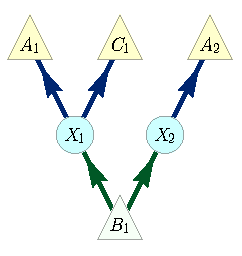
\includegraphics[scale=1]{shannonYEScopyV1.pdf}
\caption{An inflation of \cref{fig:beforecopy}.}\label{fig:aftercopy}
\end{minipage}
\end{figure}

\section{Causal compatibility inequalities for the Triangle scenario in machine-readable format}
\label{sec:38ineqs}

The following polynomial inequalities for the Triangle scenario with binary observed variables have been derived via the linear quantifier elimination method of~\cref{sec:ineqs} using the inflation DAG of~\cref{fig:Tri222}. Initially this has resulted in 64 symmetry classes of inequalities, where the symmetries are given by permuting the variables and inverting the outcomes. For the resulting 64 inequalities, numerical checks have found violations of only 37 of them: although they are all facets of the marginal polytope over the distributions on pre-injectable sets, there is no guarantee that they are also nontrivial inequalities at the level of the original DAG, and this has indeed turned out not to be the case for 26 of these symmetry classes of inequalities. Moreover, it is still likely to be the case that some of these inequalities are redundant; we have not checked whether for every inequality there is a distribution which violates the inequality but satisfies all others.

In the following table, the inequalities are listed in expectation-value form, where we assume the two possible outcomes of each variables to be $\{-1,+1\}$. Each row in the table gives the coefficients of one inequality, which is then $\geq 0$. Inequalities \#1, \#3--4, \#8--17 and \#19--24 in the table are also implied by the hypergraph transversals technique per \cref{sec:TSEM}.

\begin{table*}[ht]\centering\caption{List of inequalities as table of coefficients. This is a machine-readable version of the table in \cref{sec:CCineqs}.\medskip}\label{tab:machinereadable}
\resizebox{\textwidth}{!}{
\begin{tabular}{lc@{\hspace{1em}}ccc@{\hspace{1em}}ccc@{\hspace{1em}}c@{\hspace{1em}}ccc@{\hspace{1em}}ccc@{\hspace{1em}}c} 
  & constant & \(\expec{A}\) & \(\expec{B}\) & \(\expec{C}\) & \(\expec{A B}\) & \(\expec{A C}\) & \(\expec{B C}\) & \(\expec{A B C}\) & \(\expec{A}\expec{B}\) & \(\expec{A}\expec{C}\) & \(\expec{B}\expec{C}\) & \(\expec{C}\expec{A B}\) & \(\expec{B}\expec{A C}\) &
   {\(\expec{A}\expec{B C}\)} & {\(\expec{A}\expec{B}\expec{C}\)}   \\\bottomrule
\text{($\#$1):} & 1 & 0 & 0 & 0 & 1 & 1 & 0 & 0 & 0 & 0 & 1 & 0 & 0 & 0 & 0 \\
 \text{($\#$2):} & 2 & 0 & 0 & 0 & 0 & -2 & 0 & 0 & 0 & 0 & 0 & -1 & 0 & 0 & 1 \\
 \text{($\#$3):} & 3 & 1 & -1 & 1 & 1 & 3 & 0 & 0 & 0 & 0 & 1 & -1 & -1 & 0 & 1 \\
 \text{($\#$4):} & 3 & 1 & -1 & 1 & 1 & 3 & 0 & 0 & 0 & 0 & 1 & 1 & -1 & 0 & -1 \\
 \text{($\#$5):} & 3 & 0 & 1 & 0 & 1 & 0 & -2 & 0 & -1 & 1 & 0 & 1 & -1 & 0 & 1 \\
 \text{($\#$6):} & 3 & 0 & 1 & 0 & 0 & -2 & -2 & 0 & 0 & 1 & 0 & -1 & -1 & 0 & 1 \\
 \text{($\#$7):} & 3 & 0 & 1 & 0 & 1 & 0 & -2 & 0 & 1 & -1 & 0 & 1 & 1 & 0 & -1 \\
 \text{($\#$8):} & 3 & 1 & 1 & 1 & 2 & 2 & 2 & -1 & 1 & 1 & 1 & 1 & 1 & 1 & -1 \\
 \text{($\#$9):} & 3 & 1 & 1 & 1 & 0 & 2 & -2 & 1 & -1 & 1 & 1 & 1 & 1 & -1 & -1 \\
 \text{($\#$10):} & 4 & 0 & 0 & 2 & -2 & -2 & 0 & -1 & 2 & 0 & 2 & 1 & 1 & 1 & 0 \\
 \text{($\#$11):} & 4 & 0 & -2 & 0 & -2 & 0 & -3 & 1 & 0 & 0 & 1 & 1 & -1 & 0 & 1 \\
 \text{($\#$12):} & 4 & 0 & -2 & 0 & -2 & -2 & -3 & 1 & 0 & 2 & 1 & 1 & 1 & 0 & -1 \\
 \text{($\#$13):} & 4 & 0 & 0 & 0 & 2 & -2 & 1 & 1 & -2 & -2 & -1 & -1 & 1 & 0 & -1 \\
 \text{($\#$14):} & 4 & 0 & 0 & 0 & 2 & -2 & 1 & 1 & -2 & 2 & -1 & 1 & 1 & 0 & 1 \\
 \text{($\#$15):} & 4 & 0 & 0 & 0 & 0 & -2 & 3 & 1 & 0 & 2 & 1 & -1 & -1 & 0 & 1 \\
 \text{($\#$16):} & 4 & 0 & -2 & 0 & -2 & -2 & -2 & 1 & 0 & 2 & 0 & 1 & 1 & -1 & 0 \\
 \text{($\#$17):} & 4 & 0 & 0 & 0 & -2 & -2 & -2 & 1 & 2 & 2 & 2 & 1 & 1 & 1 & 0 \\
 \text{($\#$18):} & 5 & 1 & 1 & 1 & 3 & 1 & -4 & 0 & -2 & 0 & 1 & 1 & -1 & 0 & 1 \\
 \text{($\#$19):} & 5 & 1 & 1 & 1 & 3 & -1 & -4 & 0 & 2 & -2 & 1 & 1 & 1 & 0 & -1 \\
 \text{($\#$20):} & 5 & 1 & -1 & 1 & 1 & 2 & -2 & -2 & -2 & -1 & 1 & 1 & -2 & -2 & 0 \\
 \text{($\#$21):} & 5 & 1 & 1 & 1 & 1 & 2 & -2 & -1 & 0 & -1 & -1 & 2 & 1 & 1 & -2 \\
 \text{($\#$22):} & 5 & -1 & 1 & 1 & 1 & 1 & -1 & 1 & -2 & -2 & 2 & -2 & -2 & -2 & 0 \\
 \text{($\#$23):} & 5 & 1 & 1 & 1 & 2 & 1 & -1 & 1 & -1 & 0 & 2 & -1 & -2 & -2 & 1 \\
 \text{($\#$24):} & 5 & 1 & 1 & 1 & -1 & 2 & 2 & 1 & -2 & -1 & -1 & 2 & 1 & -1 & -2 \\
 \text{($\#$25):} & 6 & 0 & 0 & 0 & -4 & -3 & 0 & 0 & 2 & 1 & 2 & -2 & -1 & -2 & 1 \\
 \text{($\#$26):} & 6 & -2 & 0 & 2 & -5 & -3 & 0 & 0 & 1 & 1 & 0 & -1 & 1 & -2 & 2 \\
 \text{($\#$27):} & 6 & 0 & 0 & 2 & -4 & 3 & 0 & 0 & 2 & 1 & 0 & -2 & 1 & -2 & 1 \\
 \text{($\#$28):} & 6 & 0 & 0 & 0 & 1 & -3 & 2 & 0 & 1 & 1 & -4 & 1 & -1 & -2 & -2 \\
 \text{($\#$29):} & 6 & 0 & 2 & 0 & 3 & 0 & -5 & 0 & 1 & -2 & 1 & 1 & 2 & 1 & -2 \\
 \text{($\#$30):} & 6 & 0 & 2 & 0 & 2 & -2 & 1 & 0 & -2 & 4 & -1 & 2 & 2 & 1 & 1 \\
 \text{($\#$31):} & 6 & 0 & 0 & 0 & -2 & -3 & -2 & -2 & 0 & 1 & 4 & -2 & -1 & 0 & 1 \\
 \text{($\#$32):} & 7 & 1 & 1 & 1 & 2 & 1 & -3 & 3 & 1 & -2 & 2 & 3 & 2 & -2 & -1 \\
 \text{($\#$33):} & 8 & 0 & 0 & 0 & -2 & -4 & -2 & -3 & 2 & 4 & -2 & -1 & 1 & -3 & 2 \\
 \text{($\#$34):} & 8 & 2 & 0 & -2 & -6 & 1 & 0 & 1 & 0 & -1 & 2 & 1 & 2 & -3 & 3 \\
 \text{($\#$35):} & 8 & 2 & 0 & 0 & 6 & 1 & -2 & 1 & 0 & 1 & 2 & -1 & -2 & -3 & 3 \\
 \text{($\#$36):} & 8 & 0 & -2 & -2 & 0 & -6 & 1 & 1 & 2 & 0 & -1 & 3 & 1 & -2 & -3 \\
 \text{($\#$37):} & 8 & 0 & 2 & 0 & 1 & 2 & -6 & 1 & 1 & -2 & 0 & 2 & 3 & -1 & -3 
\end{tabular}}
\end{table*}


\section{Recovering the Bell inequalities from the inflation technique}
\label{sec:Bellscenarios}


To further illustrate the power of our inflation DAG approach, we now demonstrate how to recover all Bell inequalities~\cite{Brunner2013Bell,bell1966lhvm,CHSHOriginal} via our method. To keep things simple we only discuss the case of a bipartite Bell scenario with two values for both ``settings'' and ``outcome'' variables here, but the case of more parties and/or more values per variable is totally analogous.

The causal structure associated to the Bell \cite{bell1964einstein,Brunner2013Bell,bell1966lhvm,CHSHOriginal} experiment [\citealp{pusey2014gdag}~(Fig.~E\#2), \citealp{WoodSpekkens}~(Fig.~19), \citealp{chaves2014novel}~(Fig.~1), \citealp{BeyondBellII}~(Fig.~1), \citealp{wolfe2015nonconvexity}~(Fig.~2b), \citealp{steeg2011relaxation}~(Fig.~2)] is depicted in \cref{fig:NewBellDAG1}. The observed variables are $A,B,X,Y$, and $\Lambda$ is the latent common cause of $A$ and $B$. In a Bell scenario, one traditionally works with the conditional distribution $P_{AB|XY}$, to be understood as an array of distributions indexed by the possible values of $X$ and $Y$, instead of with the original distribution $P_{ABXY}$, which is what we do.

In the inflation DAG of \cref{fig:BellDagCopy1}, the maximal pre-injectable sets are
\begin{align}\begin{split}
	\label{eq:bellcontexts}
&\brackets{A_1 B_1 X_1 X_2 Y_1 Y_2}, \\
&\brackets{A_1 B_2 X_1 X_2 Y_2 Y_2}, \\
&\brackets{A_2 B_1 X_1 X_2 Y_2 Y_2}, \\
&\brackets{A_2 B_2 X_1 X_2 Y_2 Y_2},
\end{split}\end{align}
where notably every maximal pre-injectable set contains all ``settings'' variables $X_1$ to $Y_2$. The marginal distributions on these pre-injectable sets are then specified by the original observed distribution via
\begin{align}\begin{split}&\forall{a b x_1 x_2 y_1 y_2}:\; \begin{cases}
	P_{A_1 B_1 X_1 X_2 Y_1 Y_2}(a b x_1 x_2 y_1 y_2)  = P_{A B X Y}(a b x_1 y_1) P_X(x_2) P_Y(y_2), \\
	P_{A_1 B_2 X_1 X_2 Y_1 Y_2}(a b x_1 x_2 y_1 y_2)  = P_{A B X Y}(a b x_1 y_2) P_X(x_2) P_Y(y_1), \\
	P_{A_2 B_1 X_1 X_2 Y_1 Y_2}(a b x_1 x_2 y_1 y_2)  = P_{A B X Y}(a b x_2 y_1) P_X(x_1) P_Y(y_2), \\
	P_{A_2 B_2 X_1 X_2 Y_1 Y_2}(a b x_1 x_2 y_1 y_2)  = P_{A B X Y}(a b x_2 y_2) P_X(x_1) P_Y(y_1), \\
\hspace{2.5pc}	P_{X_1 X_2 Y_1 Y_2}(x_1 x_2 y_1 y_2)  = P_X(x_1) P_X(x_2) P_Y(y_1) P_Y(y_2).
\end{cases}\end{split}\end{align}
By dividing each of the first four equations by the fifth, we obtain
\begin{align}\begin{split}
	\label{eq:bellfactor}
	\forall{a b x_1 x_2 y_1 y_2}:\; \begin{cases}
	P_{A_1 B_1 | X_1 X_2 Y_1 Y_2}(a b | x_1 x_2 y_1 y_2)  = P_{A B | X Y}(a b | x_1 y_1), \\
	P_{A_1 B_2 | X_1 X_2 Y_1 Y_2}(a b | x_1 x_2 y_1 y_2)  = P_{A B | X Y}(a b | x_1 y_2), \\
	P_{A_2 B_1 | X_1 X_2 Y_1 Y_2}(a b | x_1 x_2 y_1 y_2)  = P_{A B | X Y}(a b | x_2 y_1), \\
	P_{A_2 B_2 | X_1 X_2 Y_1 Y_2}(a b | x_1 x_2 y_1 y_2)  = P_{A B | X Y}(a b | x_2 y_2).
\end{cases}\end{split}\end{align}
The existence of a joint distribution over all six variables---i.e.~the existence of a solution to the marginal problem---implies in particular
\begin{align}
	\forall{a b x_1 x_2 y_1 y_2}: \quad P_{A_1 B_1 | X_1 X_2 Y_1 Y_2}(a b | x_1 x_2 y_1 y_2)  =  \sum\nolimits_{a',b'} P_{A_1 A_2 B_1 B_2 | X_1 X_2 Y_1 Y_2}(a a' b b'|x_1 x_2 y_1 y_2),
\end{align}
and similarly for the other three conditional distributions under consideration. For compatibility with the Bell scenario, \cref{eq:bellfactor} therefore implies that the original distribution must satisfy in particular
\begin{align}\begin{split}\label{eq:finalBellstep}\forall{a b}:\; \begin{cases}
	P_{A B | X Y}(a b | 0 0)  =  \sum\nolimits_{a',b'} P_{A_1 A_2 B_1 B_2| X_1 X_2 Y_1 Y_2}(a a' b b'|0101) \\
	P_{A B | X Y}(a b | 1 0)  =  \sum\nolimits_{a',b'} P_{A_1 A_2 B_1 B_2| X_1 X_2 Y_1 Y_2}(a' a b b'|0101) \\
	P_{A B | X Y}(a b | 0 1)  =  \sum\nolimits_{a',b'} P_{A_1 A_2 B_1 B_2| X_1 X_2 Y_1 Y_2}(a a' b' b|0101) \\
	P_{A B | X Y}(a b | 1 1)  =  \sum\nolimits_{a',b'} P_{A_1 A_2 B_1 B_2| X_1 X_2 Y_1 Y_2}(a' a b' b|0101)
\end{cases}\end{split}\end{align}
The possibility to write the conditional probabilities in the Bell scenario in this form is equivalent to the existence of a latent variable model, as noted in Fine's theorem~\cite{FineTheorem}. Thus, the existence of a solution to our marginal problem implies the existence of a latent variable model for the original distribution; the converse follows from our \cref{mainlemma}. Hence the inflation DAG of~\cref{fig:BellDagCopy1} provides necessary and sufficient conditions for the compatibility of the original distribution with the Bell scenario causal structure.

Moreover, it is possible to describe the marginal polytope over the pre-injectable sets of~\cref{eq:bellcontexts}, resulting in a concrete correspondence between tight Bell inequalities and the facets of our marginal polytope. This is based on the observation that the ``settings'' variables $X_1$ to $Y_2$ occur in all four contexts. The marginal polytope lives in $\oplus_{i=1}^4 \mathbb{R}^{2^6} = \oplus_{i=1}^4 (\mathbb{R}^2)^{\otimes 6}$, where each tensor factor has basis vectors corresponding to the two possible outcomes of each variable, and the direct summands enumerate the four contexts. It is given by the convex hull of the points
\begin{align*}
	(e_{A_1} & \otimes e_{B_1} \otimes e_{X_1} \otimes e_{X_2} \otimes e_{Y_1} \otimes e_{Y_2}) \\
	\oplus\: (e_{A_1} & \otimes e_{B_2} \otimes e_{X_1} \otimes e_{X_2} \otimes e_{Y_1} \otimes e_{Y_2}) \\
	\oplus\: (e_{A_2} & \otimes e_{B_1} \otimes e_{X_1} \otimes e_{X_2} \otimes e_{Y_1} \otimes e_{Y_2}) \\
	\oplus\: (e_{A_2} & \otimes e_{B_2} \otimes e_{X_1} \otimes e_{X_2} \otimes e_{Y_1} \otimes e_{Y_2}),
\end{align*}
where all six variables range over their possible values. Since the last four tensor factors occur in every direct summand in exactly the same way, we can also write the point as
\[
	\left[ (e_{A_1} \otimes e_{B_1}) \oplus (e_{A_1} \otimes e_{B_2}) \oplus (e_{A_2} \otimes e_{B_1}) \oplus (e_{A_2} \otimes e_{B_2})\right] \otimes \left[ e_{X_1} \otimes e_{X_2} \otimes e_{Y_1} \otimes e_{Y_2}\right]
\]
in $\big(\oplus_{i=1}^4 \mathbb{R}^{2^2}\big)\otimes \mathbb{R}^{2^4}$. Now since the first four variables in the first tensor factor vary completely independently of the latter four variables in the second tensor factor, the resulting polytope will be precisely the tensor product~\cite{namioka_tensor_1969,bogart_hom_2013} of two polytopes: first, the convex hull of all points of the form
\[
	(e_{A_1} \otimes e_{B_1}) \oplus (e_{A_1} \otimes e_{B_2}) \oplus (e_{A_2} \otimes e_{B_1}) \oplus (e_{A_2} \otimes e_{B_2}),
\]
and second the convex hull of all $e_{X_1} \otimes e_{X_2} \otimes e_{Y_1} \otimes e_{Y_2}$. While the latter polytope is just the standard probability simplex in $\mathbb{R}^8$, the former cone is precisely the ``local polytope'' or ``Bell polytope'' that is traditionally used in the context of Bell scenarios~\cite[Sec.~II.B]{Brunner2013Bell}. This implies that the facets of our marginal polytope are precisely the pairs consisting of a facet of the Bell polytope and a facet of the simplex, the latter of which are only the nonnegativity of probability inequalities like $P_{X_1X_2Y_1Y_2}(0101)\geq 0$. For example, in this way we obtain one version of the CHSH inequality as a facet of our marginal polytope,
\[
	\sum_{a,b,x,y} (-1)^{a + b + xy} P_{A_x B_y X_1 X_2 Y_1 Y_2}(a b 0 1 0 1) \leq 2 P_{X_1 X_2 Y_1 Y_2}(0101).
\]
This translates into the standard form of the CHSH inequality as follows. Upon using~\cref{eq:bellfactor}, the inequality becomes
\begin{align*}
	\sum_{a,b} (-1)^{a + b} \big( & P_{A B X Y}(ab00)P_X(1)P_Y(1) + P_{A B X Y}(ab01)P_X(1)P_Y(0) \\[-4pt]
	& + P_{A B X Y}(ab10)P_X(0)P_Y(1) - P_{A B X Y}(ab11)P_X(0)P_Y(0) \big) \leq P_X(0)P_X(1)P_Y(0)P_Y(1),
\end{align*}
so that dividing by the right-hand side results in one of the conventional forms of the CHSH inequality,
\[
	\sum_{a,b} (-1)^{a + b} \left( P_{AB|XY}(ab|00) + P_{AB|XY}(ab|01) + P_{AB|XY}(ab|10) - P_{AB|XY}(ab|11) \right) \leq 2.
\]
In conclusion, the inflation technique is powerful enough to get a precise characterization of all distributions compatible with the Bell causal structure, and our technique for generating polynomial inequalities through solving the marginal constraint problem recovers all Bell inequalities.

Some Bell inequalities may also be derived using the hypergraph transversals technique discussed in \cref{sec:TSEM}. For example, the inequality
\begin{align}\label{eq:preBell}\begin{split}
& \p[A_1 B_1 X_1 Y_1]{0000}\p[X_2]{1} \p[Y_2]{1} \\
&\leq
 \p[A_1 B_2 X_1 Y_2]{0001}\p[X_2]{1} \p[Y_1]{0} +\p[A_2 B_1 X_2 Y_1]{0010}\p[X_1]{0}\p[Y_2]{1}+  \p[A_2 B_2 X_2 Y_2]{1111}\p[X_1]{0} \p[Y_1]{0}
\end{split}\end{align}
is the inflationary precursor of the Bell inequality
\begin{align}\label{eq:aBell}
 \p[A B | X Y]{00|00} &\leq \p[A B | X Y]{00|01} +\p[A B | X Y]{00|10}+  \p[A B | X Y]{11|11},
\end{align}
as \cref{eq:aBell} is obtained from \cref{eq:preBell} by dividing both sides by $\p[X_1 Y_1 X_2 Y_2]{0011}=\p[X_1]{0} \p[Y_2]{0}\p[X_2]{1} \p[Y_2]{1}$ and then dropping copy indices. On the other hand, \cref{eq:preBell} follows directly from factorization relations on pre-injectable sets and the tautology
\begin{align}\begin{split}
	[ \mgreen{A_1 \eql 0}, & \mgreen{B_1 \eql 0}, \mgreen{X_1 \eql 0}, \mgreen{Y_1\eql 0}, \mgreen{X_2 \eql 1}, \mgreen{Y_2 \eql 1}]\\
 \implies 
	[ & \mgreen{A_1 \eql 0}, B_2 \eql 0, \mgreen{X_1 \eql 0}, \mgreen{Y_1\eql 0}, \mgreen{X_2 \eql 1}, \mgreen{Y_2 \eql 1}] \\
	\mathrel{\lor} [ & A_2 \eql 0, \mgreen{B_1 \eql 0}, \mgreen{X_1 \eql 0}, \mgreen{Y_1\eql 0}, \mgreen{X_2 \eql 1}, \mgreen{Y_2 \eql 1}] \\
	\mathrel{\lor} [ & A_2 \eql 1, B_2 \eql 1, \mgreen{X_1 \eql 0}, \mgreen{Y_1\eql 0}, \mgreen{X_2 \eql 1}, \mgreen{Y_2 \eql 1}].
\end{split}\end{align}
which corresponds to the original ``Hardy paradox''~\cite{L.Hardy:PRL:1665} in our notation.




\renewcommand\section{\stdsection}
\let\cleardoublepage\clearpage
\setlength{\bibsep}{3pt plus 3pt minus 2pt}
\bibliographystyle{apsrev4-1}
\nocite{apsrev41Control}
\bibliography{hardyinference}
\end{document}
